%% This is file `elsarticle-template-1-num.tex',
%%
%% Copyright 2009 Elsevier Ltd
%%
%% This file is part of the 'Elsarticle Bundle'.
%% ---------------------------------------------
%%
%% It may be distributed under the conditions of the LaTeX Project Public
%% License, either version 1.2 of this license or (at your option) any
%% later version.  The latest version of this license is in
%%    http://www.latex-project.org/lppl.txt
%% and version 1.2 or later is part of all distributions of LaTeX
%% version 1999/12/01 or later.
%%
%% The list of all files belonging to the 'Elsarticle Bundle' is
%% given in the file `manifest.txt'.
%%
%% Template article for Elsevier's document class `elsarticle'
%% with numbered style bibliographic references
%%
%% $Id: elsarticle-template-1-num.tex 149 2009-10-08 05:01:15Z rishi $
%% $URL: http://lenova.river-valley.com/svn/elsbst/trunk/elsarticle-template-1-num.tex $
%%
\documentclass[english,preprint,12pt]{elsarticle}

%% Use the option review to obtain double line spacing
%% \documentclass[preprint,review,12pt]{elsarticle}

%% Use the options 1p,twocolumn; 3p; 3p,twocolumn; 5p; or 5p,twocolumn
%% for a journal layout:
%% \documentclass[final,1p,times]{elsarticle}
%% \documentclass[final,1p,times,twocolumn]{elsarticle}
%% \documentclass[final,3p,times]{elsarticle}
%% \documentclass[final,3p,times,twocolumn]{elsarticle}
%% \documentclass[final,5p,times]{elsarticle}
%% \documentclass[final,5p,times,twocolumn]{elsarticle}

%% if you use PostScript figures in your article
%% use the graphics package for simple commands
%% \usepackage{graphics}
%% or use the graphicx package for more complicated commands
%% \usepackage{graphicx}
%% or use the epsfig package if you prefer to use the old commands
%% \usepackage{epsfig}

%% The amssymb package provides various useful mathematical symbols
\usepackage{amssymb}
%% The amsthm package provides extended theorem environments
%% \usepackage{amsthm}

\usepackage{stmaryrd}
\usepackage{color}

%% The lineno packages adds line numbers. Start line numbering with
%% \begin{linenumbers}, end it with \end{linenumbers}. Or switch it on
%% for the whole article with \linenumbers after \end{frontmatter}.
%% \usepackage{lineno}

%% natbib.sty is loaded by default. However, natbib options can be
%% provided with \biboptions{...} command. Following options are
%% valid:

%%   round  -  round parentheses are used (default)
%%   square -  square brackets are used   [option]
%%   curly  -  curly braces are used      {option}
%%   angle  -  angle brackets are used    <option>
%%   semicolon  -  multiple citations separated by semi-colon
%%   colon  - same as semicolon, an earlier confusion
%%   comma  -  separated by comma
%%   numbers-  selects numerical citations
%%   super  -  numerical citations as superscripts
%%   sort   -  sorts multiple citations according to order in ref. list
%%   sort&compress   -  like sort, but also compresses numerical citations
%%   compress - compresses without sorting
%%
%% \biboptions{comma,round}

% \biboptions{}

\usepackage{listings}
\usepackage{bold-extra}
\usepackage{url}
\usepackage{babel}
\usepackage{array}
\usepackage{graphicx}
\usepackage{subfig}
\usepackage{multirow}
\usepackage{comment}

\lstdefinelanguage{ocaml}{
keywords={let, begin, end, in, match, type, and, fun, function, try, with, class, object, method, of, rec, repeat, until,
          while, not, do, done, as, val, inherit, module, sig, deriving, datatype, struct, if, then, else, ostap},
sensitive=true
}

\lstdefinelanguage{oberon0}{
keywords={MODULE, END, PROCEDURE, VAR, TYPE, CONST, FOR, WHILE, CASE, IF, BEGIN, ELSIF, THEN, ARRAY, OF, RECORD, DO},
sensitive=true
}

\newcommand{\oberonsize}{\fontsize{9pt}{9pt}}
\lstnewenvironment{oberon0} {\lstset{language={oberon0}}\oberonsize}{}
\newcommand\textoberon[1]{{\lstinline[language={oberon0}]{#1}}}
\newcommand\textoberonF[1]{{\oberonsize\lstinline[language={oberon0}]{#1}}}

\lstdefinelanguage{scala}{
   keywords={abstract,case,catch,class,def,do,else,extends,false,final,
     finally,for,forSome,if,implicit,import,lazy,match,new,null,
     object,override,package,private,protected,requires,return,
     sealed,super,this,throw,trait,try,true,type,val,var,while,
     with,yield},
   sensitive=true
}

\newcommand{\scalasize}{\fontsize{9pt}{9pt}}
\lstnewenvironment{scala} {\lstset{language={scala}}\scalasize}{}
\newcommand\textscala[1]{{\lstinline[language={scala}]{#1}}}
\newcommand\textscalaF[1]{{\scalasize\lstinline[language={scala}]{#1}}}

\lstset{
basicstyle=\small\ttfamily,
identifierstyle=\ttfamily,
keywordstyle=\ttfamily\bfseries,
commentstyle=\scriptsize\rmfamily,
basewidth={0.5em,0.5em},
fontadjust=true
}

\journal{Science of Computer Programming}

%%%% Rascal needed stuff
\usepackage{xspace,rascal/rascal,float}
%\floatstyle{ruled}
\newfloat{listing}{htbp}{lol}
\floatname{listing}{Listing}
%%%% End Rascal needed stuff

\begin{document}

\begin{frontmatter}

%% Title, authors and addresses

%% use the tnoteref command within \title for footnotes;
%% use the tnotetext command for the associated footnote;
%% use the fnref command within \author or \address for footnotes;
%% use the fntext command for the associated footnote;
%% use the corref command within \author for corresponding author footnotes;
%% use the cortext command for the associated footnote;
%% use the ead command for the email address,
%% and the form \ead[url] for the home page:
%%
%% \title{Title\tnoteref{label1}}
%% \tnotetext[label1]{}
%% \author{Name\corref{cor1}\fnref{label2}}
%% \ead{email address}
%% \ead[url]{home page}
%% \fntext[label2]{}
%% \cortext[cor1]{}
%% \address{Address\fnref{label3}}
%% \fntext[label3]{}

\title{LDTA Tool Challenge}

%% use optional labels to link authors explicitly to addresses:
%% \author[label1,label2]{<author name>}
%% \address[label1]{<address>}
%% \address[label2]{<address>}

\author[tue]{Mark van den Brand}

% Please add your names below, we can sort out the order later.

\author[umn]{Eric Van Wyk}
\author[umn]{Ted Kaminski}

\author[lu]{Niklas Fors}
\author[lu]{G{\"o}rel Hedin}
\author[cwi]{Tijs van der Storm}

\author[mq]{Anthony M. Sloane}

\author[cy]{Margus Freudenthal}

\author[spbu]{Dmitry Boulytchev}

\author[uu]{Doaitse Swierstra}

\author[udelar]{Marcos Viera}


\address[tue]{Technical University of Eindhoven, Eindhoven, The Netherlands}
\address[umn]{University of Minnesota, Minneapolis, MN, United States}
\address[lu]{Lund University, Lund, Sweden}
\address[mq]{Macquarie University, Sydney, Australia}
\address[cy]{Cybernetica AS / University of Tartu, Tartu, Estonia}
\address[spbu]{St-Petersburg State University, St.Petersburg, Russia}
\address[cwi]{Centrum Wiskunde \&\ Informatica, Amsterdam, The Netherlands}
\address[uu]{Utrecht University, Utrecht, The Netherlands}
\address[udelar]{University of the Republic, Montevideo, Uruguay}

\begin{abstract}

An abstract goes here...

\end{abstract}

\begin{keyword}
%% keywords here, in the form: keyword \sep keyword

%% MSC codes here, in the form: \MSC code \sep code
%% or \MSC[2008] code \sep code (2000 is the default)

\end{keyword}

\end{frontmatter}

%%
%% Start line numbering here if you want
%%
% \linenumbers

%% main text
\section{Introduction}
\label{sec:intro}

\begin{itemize}
\item How to read the paper?
\item Systems involved
\item Scanning and parsing
\item Name analysis and type checking
\item Source to source translation and code generation
\item Handling of artifacts
\end{itemize}

\section{Oberon-0}
\label{sec:oberon}

Oberon-0 is an imperative programming language designed by Niklaus Wirth for his compiler construction book~\cite{Wirth96}.
Wirth's aim was to have a simple, yet familiar language, containing enough fundamental constructs to require most standard compilation techniques.
The language contains a standard collection of imperative features: constants; basic, array and record types; variables; expressions; assignment, conditional and while statements; and procedures with both value and variable parameter passing modes.
Figure~\ref{fig:oberonexample} shows a simple Oberon-0 program that reads a number and prints its multiples up to ten.
More Oberon-0 examples can be found in \ref{sec:samples}.

\begin{figure}[t]
\begin{oberon0}
MODULE Multiples;

CONST
  limit = 10;

VAR
  base, count : INTEGER;
  mult : INTEGER;

PROCEDURE calcmult (i : INTEGER; base : INTEGER;
                    VAR result : INTEGER);
BEGIN
  result := i * base
END calcmult;

BEGIN
  Read (base);
  FOR count := 1 TO limit DO
    calcmult (count, base, mult);
    Write (mult);
    WriteLn
  END
END Multiples.
\end{oberon0}
\caption{An Oberon-0 program to read a number \texttt{base} and print out its successive multiples up to ten.}
\label{fig:oberonexample}
\end{figure}

As can be seen from the examples, Oberon-0 lives in Wirth's Pascal family of languages and is most closely related to Oberon.
It does not have any of the procedure variable or record extension features of the later languages in that family, nor any of the modularity features of earlier languages such as Modula-2.

Compilation of Oberon-0 was chosen as the subject for the LDTA Tool Challenge for two main reasons.
First, the language and techniques for compiling it were sufficiently standard that the participants did not have to learn a new problem domain.
While a more complex task might be preferable in some sense, for this challenge we felt it was best to have a familiar, tractable problem space.
Second, the existence of Wirth's book meant that a resource already existed to describe the language.
The book contains a compiler implementation which we used as a reference implementation.

Unfortunately, both the book's description of Oberon-0 and the implementation proved to be incomplete, so on a few occasions we resorted to defining the desired behaviour ourselves.
For example, the language description implies that scopes can be arbitrarily nested, but the implementation does not handle this generality.
For the challenge we agreed to follow the reference implementation, although many of our implementations are more general.

The challenge was to implement a compiler for Oberon-0.
We broke the task down into smaller sub-tasks so that participants could choose how much to implement.
Also, we aimed to demonstrate different techniques for modularity of language implementation.
Therefore, we first defined different language levels within the full Oberon-0 definition.
A language level comprises a set of features that must be implemented.
We then defined language processing tasks that apply to any language.
A task comprises a particular processing activity.
Table~\ref{tab:levelstasks} lists the language levels and tasks.\footnote{At early stages of the challenge, tasks 4 and 5 were split to include optimisation and RISC code generation, respectively. These tasks were dropped later since they were orthogonal to the main aim of the challenge.}

\begin{table}\centering
\begin{tabular}{|cl|} \hline
\multicolumn{2}{|c|}{\emph{Language levels}} \\ \hline
L0 & Basic constants, types and variables      \\
   & simple expressions, assignment statements \\ \hline
L1 & Add \verb|IF| and \verb|WHILE| statements \\ \hline
L2 & Add \verb|FOR| and \verb|CASE| statements \\ \hline
L3 & Add procedures                            \\ \hline
L4 & Add arrays and records                    \\ \hline
\multicolumn{2}{c}{} \\ \hline
\multicolumn{2}{|c|}{\emph{Processing tasks}} \\ \hline
T1 & parsing and pretty printing \\ \hline
T2 & name analysis \\ \hline
T3 & type analysis \\ \hline
T4 & desugaring \\ \hline
T5 & C code generation \\ \hline
\end{tabular}
\caption{Language levels and processing tasks used in the challenge.}
\label{tab:levelstasks}
\end{table}

Any combination of a language level and task constitutes an artifact that could be constructed.
For example, choosing L2 and T3 we obtain an artifact that can type check programs containing up to \verb|FOR| and \verb|CASE| statements, but does not support procedures or structured types, and cannot generate code.
For the challenge, we specified four combinations on which participants were to focus (Table~\ref{tab:artifacts}).
These combinations were chosen to control the complexity of the challenge, but also to be representative of a progression that a real implementation might go through.
Our aim was to enable participants to demonstrate the modularity of their approaches in a variety of realistic situations.

\begin{table}\centering
\begin{tabular}{|c|c|c|l|} \hline
\emph{Artifact} & \emph{Language} & \emph{Tasks} & \\ \hline
A1  & L2 & T1-2 & Core language with pretty printing and \\
    &    &      & name binding \\ \hline
A2a & L3 & T1-2 & A1 plus syntax and name binding for \\
    &    &      & procedures \\ \hline
A2b & L2 & T1-3 & A1 plus type checking \\ \hline
A3  & L3 & T1-3 & A2a and A2b \\ \hline
A4  & L4 & T1-5 & Full language and all tasks \\ \hline
\end{tabular}
\caption{The artifacts that were developed during the challenge.}
\label{tab:artifacts}
\end{table}


% 3--8 Systems
% Please add an input line below for your paper section.  We can sort
% out the order of these later.

\newpage
\newcommand{\code}[1]{\texttt{#1}}

\section{Silver, a meta-language for language extension}

\subsection{Introduction to Silver}

Silver is an extensible attribute grammar system that
supports many modern attribute grammar features.  These include
higher-order\cite{vogt89}, reference~\cite{hedin00informatica}, and a
simplified notion of collection attributes~\cite{boyland05}.
%
Silver introduced \emph{forwarding} into an attribute grammar
setting~\cite{vanwyk02}, a mechanism that is useful for specifying
composable language extensions.
%
It also has a module system and supports separate compilation.
%
Silver is distributed with and coupled to Copper, an integrated parser
and context-aware scanner generator~\cite{vanwyk07gpce}.  As a
language, Silver has specific syntax for specifying the concrete and
lexical syntax of the object language.
%
In addition, Silver's type system supports parametric polymorphism and
a limited form of type inference which allows one to write lazy
functional programs in Silver~\cite{kaminski11sle}.



We have found Silver to be a convenient and expressive way to implement
translators for a variety of languages.  The main purpose for
developing Silver and Copper is to investigate extensible languages in
which a \emph{host language} is composed with a set of
independently-developed \emph{language extensions}.  This composition
of specifications of these components is to be performed automatically
by Silver and Copper and can thus be done at the direction of a
non-expert programmer.

Silver is both a (meta) language for language specifications, as well
as a tool that translates AG specifications to Java and concrete
syntax specifications to the input language for Copper.  Copper
generates the scanner and parser as Java code as well.  The resulting
Java code is compiled and packaged into a JAR file.  Silver
(implemented as a Silver specification) and Copper are both
distributed in source form under the LGPL licences and as executable
Java Jar files, making installation simple.


\paragraph{The organization of the Oberon0 specification in Silver}

To demonstrate Silver's support for highly modular language design, the
Oberon0 specification is organized in many different Silver modules,
called grammars.
%
A grammar can contain lexical and concrete syntax specifications as
well as attribute grammar specifications for defining language
semantics, optimizations, and translations.  
%
A Silver grammar can be organized hierarchically in a directory
structure and grammar names match this structure.  
%
%A grammar is composed of the specifications in all Silver files
%(ending with a \code{.sv} extension) in a directory, and the scope of
%specifications in one file include all other files in that grammar.
%
Grammars can \code{import} and \code{export} specifications from other grammars to
create grammar specifications that are composed of multiple grammars. 
%
Thus a language designer has a high degree of flexibility in how he or
she organizes the language specifications.

\begin{figure}
\begin{verbatim}
core
  concreteSyntax, abstractSyntax, typeChecking
constructs
  controlFlow, dataStructures, procedures  
    concreteSyntax, abstractSyntax, typeChecking
tasks
  codegenC
    core, dataStructures, procedures
components
  L1, L2, L3, L4, L5, T1, T2, T3, T5
artifacts
  A1, A2a, A2b, A3, A4, A5
\end{verbatim}
\caption{The directory structure of the Oberon0 specifications.}
\label{silver:fig:structure}
\end{figure}

The directory/grammar hierarchy for the Silver specifications for
Oberon0 (contained in a directory named \code{Oberon0}) is shown in
Figure~\ref{silver:fig:structure}.  The specifications for the Oberon0
language constructs in the languages L1 to L5 and the specifications
for the language processing tasks T1 to T5 are organized across three
directories in the \code{Oberon0} directory: \code{core},
\code{constructs}, and \code{tasks}.
%
The \code{core} directory contains grammars with specifications for
the language L1 and tasks T1, T2, and T3.
%
In it, the L1 lexical and concrete syntax specifications and the T1 pretty
printing task specifications are in the grammar in
\code{concreteSyntax}, the abstract syntax and T2 name analysis task
is in the grammar \code{abstractSyntax}, and the type checking task
(T3) is specified in the \code{typeChecking} directory.
%
This illustrates one possible organization of the specifications.  Of
interest is that attributes implementing name analysis are written
on the grammar productions defining the abstract syntax, so-called
\emph{abstract productions}, while the type
checking attributes for these productions are defined in so-called
\emph{aspect productions} which allow one to define new attributes for
existing grammar productions.

The \code{constructs} directory defines the languages features that
are added to create language level L2 (\code{controlFlow}), L3
(\code{dataStrucutes}), and L4 (\code{procedures}) and these are 
organized in the same manner as the L1 specification in \code{core}.
%
This organization is inverted in the \code{tasks/codegenC} directory
in which the C code generation task specification is separate from all
language construct definitions and it is split so the specifications
for this task for language constructs for language L1, L3, and L4 are
in different grammars (\code{core}, \code{dataStructures},
\code{procedures}).

What is missing from \code{tasks/codegenC} are specifications for code
generation for the for-loop and case-statement L2 constructs.  As we
will see in Section~\ref{silver:sec:transformation}, the C code
translation of these features come for free from the use of
forwarding.  The for-loop indicates that it is semantically equivalent
to a while-loop (in the core language) and automatically gets its C
code translations from that construct.  Thus the T5 code generation task
and the L2 control flow constructs are independent of one another.

The grammars in \code{components} directory compose the relevant
grammars from \code{core}, \code{constructs}, and \code{tasks} to form
the specific languages (L1 through L5) and tasks (T1 to T5).  The
\code{artifacts} directory contains grammars for the specific
artifacts A1 to A5 which do little more than import the appropriate
grammars from the components directory.  
%
Grammar composition is essentially the set union of the different
types of specifications in the various modules.
%
These grammars and the composition process are discussed in more
detail in Section~\ref{silver:sec:artifacts}


\subsection{Scanning and parsing}

Silver is coupled to our integrated parser and context-aware scanner
generator, Copper, and allows concrete and lexical syntax
specifications to be written in the same grammar modules as the
attribute grammar specifications.  These specifications are collected
and passed to Copper for analysis and generation of a context-aware
scanner and slightly modified LALR(1) parser that is used in the
resulting AG evaluator generated by Silver.

Copper has two distinguishing characteristics.  First, Copper generates
context-aware scanners~\cite{vanwyk07gpce} which use contextual
information to dis-ambiguate lexical syntax.
%
The parser uses a slightly modified LR- style algorithm that passes to
the scanner the set of valid symbols that the scanner may return at
that point in parsing. This set consists of the terminals whose
entries in the parse table for the current parse state are
\emph{shift}, \emph{reduce}, or \emph{accept}, but not \emph{error}.
The scanner will only return tokens in this set and a static analysis
ensures there are no lexical ambiguities; thus at most one token will
ever be returned from the scanner.

This type of scanning allows terminals that appear in different
parsing contexts to have overlapping regular expressions.  This is
especially useful when parsing and scanning extensible languages in
which domain specific languages can be embedded since the host and
embedded languages may have overlapping lexical syntax.  More
generally, this means that terminal symbols do not need to be
overloaded, instead different terminal symbols can be specified with
overlapping regular expressions.  This means that they are not
overloaded in the parser and thus parse table conflicts are less
likely to occur~\cite{vanwyk07gpce}.

Second, Copper comes with a modular determinism
analysis~\cite{schwerdfeger09pldi} that lets extension writers check
the concrete and lexical syntax specification of their extension to
ensure that the composition of the host language and any other
extensions verified by this analysis will be free of conflicts and
lexical ambiguities.  That is, the parser and scanner generated from
the composition ``just works.''

%  These are explained in more detail below when describing specific
%  Oberon0 specifications.

\paragraph{Sample specifications - lexical syntax}
While the scanning and parsing techniques used by Copper are different
from others, the structure of the specifications are quite familiar.
%
Specifications for lexical syntax consist primarily of terminal symbol
declarations, which, as expected, name the terminal symbol and provide
the defining regular expression.  In the Silver specification, the
\code{Id\_t} terminal specifies variable names:

\noindent
\verb!terminal Id_t /[A-Za-z][A-Za-z0-9]*/ ;!

Terminals such as keywords, punctuation, and operators, whose regular
expressions match only one string can specify the regular expression
as a string in single quotes as is done below for the assignment and
addition operator terminal symbols:

\noindent
\verb!terminal Assign_t ':='  ;! \\
\verb!terminal Plus_t   '+'  precedence = 11, association = left;! \\
%
Such terminals can be used in concrete productions by writing the
string in single quotes instead of using the terminal, which is
sometimes more convenient and can improve the readability of the
productions. 
%
This example also shows the use of traditional precedence and
associativity specifications.

Copper supports a notion of lexical precedence, for disambiguating
keywords from variables, for example, and the specification of
white-space and comments with a \code{ignore} modifier that indicates
a terminal is not to be passed on to the parser.


\paragraph{Sample specifications - concrete syntax}
Specifications for concrete syntax also have a familiar structure.
Figure~\ref{silver:fig:concrete} shows the specification of the two
for-loop constructs added in language L2.
\begin{figure}
\begin{verbatim}
concrete productions s::Stmt_c
 | 'FOR' id::Name_c ':=' lower::Expr_c 'TO' upper::Expr_c
                    'DO' body::Stmts_c 'END'         
  { s.ast = forStmt(id.ast, lower.ast, upper.ast, body.ast); }
 | 'FOR' id::Name_c ':=' lower::Expr_c 'TO' upper::Expr_c
                    'BY' step::Expr_c 'DO' body::Stmts_c 'END' 
  { s.ast = forStmtBy(id.ast, lower.ast, upper.ast, step.ast, 
                      body.ast); }
\end{verbatim}
\caption{Concrete syntax specifications for the for-loop.}
\label{silver:fig:concrete}
\end{figure}
These productions are written in the more-or-less familiar BNF-style.
Nonterminals and terminal symbols can be named and used in the
attribute definitions that can decorate concrete productions.  Here the
higher-order synthesized \code{ast} attribute is used to construct
ASTs.  Attribute definitions are specified between the curly braces
following the production definition.
%
For the first production, the abstract for-loop AST is stored
in the \code{ast} attribute of the left hand side nonterminal named
\code{s}. Since punctuation, for example \code{:=}, and keywords do
not appear in the AST, they are specified here using only the constant
lexeme in single quotes that was given in the definition of that
terminal symbol.

As we will see below, productions defining the abstract syntax of the
language differ from concrete production in only three ways: they use
the \code{abstract} modifier instead of \code{concrete}, they are named
unlike the anonymous productions shown in
Figure~\ref{silver:fig:concrete}, and they are not passed to Copper to
be used to generate a parser.  Otherwise there is no distinction
between the two in Silver.  Thus, one can define all the semantics of
the language on the concrete syntax tree if desired.  For Oberon0 we
chose to use a separate abstract syntax, primarily for demonstration
purposes.



\subsection{Name analysis}

Name analysis in the Silver implementation of Oberon0 proceeds in a standard
way: an environment exists to look up symbols, it's extended by declarations,
and consulted to report redeclarations or undefined symbols.
%
The environment is represented by the \texttt{env} inherited
 \footnote{Actually it is an 'autocopy' attribute, this is simply an inherited attribute
 that implicitly copies from parent to child if no other definition is present.}
attribute.
%
% TODO: should we be making references to where these are in the code?
%
The \texttt{Env} type is simply a container for the separate namespaces of the
environment.
%
Each names space (e.g. the \texttt{values} attribute on \texttt{Env}) has the
type \texttt{[TreeMap<String  Decorated Decl>]}.
%
The list represents \textit{scopes}, while the map allows looking up bound
names.

This representation is actually ``over powered" for Oberon0's needs.
%
Ober-on0 does not have separate namespaces for values and types, so our
separation of them in the environment is actually unnecessary, and in fact
adds a small complication to redeclaration checks: they must consult both
namespaces.
%
However, it is a nice demonstration of how a more interesting environment
would be set up.

%\paragraph{Extensible Records.}
%
% TODO: discuss whether we should have this section on how the environment is
% set up in a way that allows new namespaces to be added by extensions, making
% it, in effect, an extensible environment.

\paragraph{Decorated types}
The result type of looking up a name in the environment -- \texttt{Decorated Decl} --
is a \textit{reference attribute} to the node in the tree that declared that name.
%
Binding names to declaration sites is a relatively standard use for
reference attributes.
%
% TODO: we can cite JastAdd doing the same thing, probably, when we see their impl
%
Whereas a higher-order attribute only represents the \textit{structure} of
a tree, a reference attribute is actually a direct reference to an existing,
attributed, node in the tree.
%
Typically, reference attributes come along with some features for manipulating
them, such as \textit{remote attributes}.
%
Silver, however, treats them in a purely functional way; they can only be
consulted for the values of their attributes, and cannot be affected in
any way.
%
Reference attributes remain extremely useful, however, as this simplifies
many kinds of environment lookups.
%
For example, as we will see later, type checking and renaming transformations
can all proceed with no modifications to the environment: they simply consult
different attributes on the declaration node.

\paragraph{Specifications in a functional style}
The function \code{lookupType} is used to retrieve the reference to a
variable's declaration, if it exists, given the variables name and
environment.  The result \code{Maybe} type is constructed from either
a \code{nothing} or a \code{just} production.   This function is shown below:
\begin{verbatim}
function lookupType
Maybe<Decorated Decl> ::= s::String e::Decorated Env
{ return foldr(orElse, nothing(), lookupInScopes(s, e.types)); }
\end{verbatim}
It folds up the results of looking for the name \code{s} in all the
scopes in the the environment using a base-value of \code{nothing} and
combining results with \code{orElse} to return the first result from
\code{lookupInScopes} that is not a \code{nothing()}.
%
The function \code{lookupInScopes}, shown below,
\begin{verbatim}
function lookupInScopes
[Maybe<a>] ::= s::String ss::[TreeMap<String a>]
{ return map(adapt, map(treeLookup(s,_), ss)); }
\end{verbatim}
uses two applications of a
traditional polymorphic \code{map} function on the results of looking
up values in the underlying \code{TreeMap} structures.  (The
\code{adapt} function converts a list of values to a \code{nothing()}
if the list is empty or a \code{just} of the first element of the list.
Thanks to laziness, it's not inefficient to use this, as we'll only
actually do the lookup as far as gets demanded in the scope list.
This style of programming is quite familiar to functional programmers
and demonstrates the use of parametric polymorphism and higher-order
functions in Silver.


\paragraph{Collection attributes}
Silver's composition model allows extensions to \textit{safely} add new attributes
to existing nonterminals, as well as new productions, so long as those productions forward
to existing host language productions.
%
% This is very powerful.
%
It's worth noting that this is not easily possible
with objects nor algebraic datatypes, and is frequently called ``the expression
problem."
%
However, it's not a complete picture of composition.
%
Extensions may need to affect existing host language attributes in some ways.

The simplest example is error reporting: the host language defines a synthesized
attribute called \texttt{errors} that is simply a list of error messages.
%
However, extensions may need to add new error messages.
%
This is particularly apparent with our implementation, as type checking is
implemented separately from the core host language.

Silver provides a notion of \textit{collection attributes} that permits this.
%
Collection attributes are ordinary attributes that come with a
\textit{composition operator}, for example the \texttt{errors} attribute
is defined with the \texttt{++} (list append) operator:
%
\begin{verbatim}
synthesized attribute errors :: [Message] with ++;
\end{verbatim}
%
The term ``collection attribute" is somewhat overloaded, coming initially
from Boyland's remote attributes~\cite{boyland05}.
%
Silver's collection attributes do not permit any remote contribution across
the tree, however.
%
Instead, they are purely within one production, and contributions instead come
from all aspects of that production, along with an initial ``base" definition:
\begin{verbatim}
abstract production not
e::Expr ::= e1::Expr
{ e.errors := e1.errors;  -- Other attributes omitted
}
\end{verbatim}
%
% Thus, one could imagine a ``aspect weaving" phase of compiling a Silver
% program, where afterwards collections attributes have been ``erased" into
% normal attributes.
%
% The erased attribute equation would then look something like
% \texttt{foldr(compositionOperator, baseDef, [contribs...])},
% where the \texttt{contribs} list is has no specified order.
The final value of the collection attribute is equivalent to the
expression \texttt{foldr (} \emph{compositionOperator}\texttt{,}
    \emph{baseDefinition}\texttt{, [} \emph{contributions} \texttt{] )}.

This design is intended to tightly control the possible misbehavior of
extensions.
%
Extensions are forbidden from doing anything ``dangerous" by default,
and the host language can poke well-defined holes to permit specific
kinds of extension behavior.


\subsection{Type checking}

Typechecking is implemented separately from the host language, as some artifacts
lack it.
%
The typechecking extensions take the following form:
\begin{itemize}
\item A new attribute \texttt{type} occurs on \texttt{Decl}, and so can be
 consulted from the reference attribute returned by a name lookup in the
 environment.
\item That attribute is a new type called \texttt{TypeRep} that is a type
 representation, distinct from \texttt{TypeExpr} which represents program
 text of a type. Put another way, \texttt{TypeExpr} may need to look up things
 in the environment, and as a result yields a \texttt{TypeRep} which is totally
 self-contained.
\item Aspects for productions in the host language consult the environment
 and use the \texttt{errors} collection attribute to add error messages
 for type errors, for example with the previously mentioned \texttt{not} production:
\begin{verbatim}
  e.errors <- checkErrors(e1.type, booleanType(), 
                          "Operand to ~", e1.location);
\end{verbatim}
The function \code{checkErrors} returns a list containing a message if
the first two types do not match; the list is empty if they do.

\item Type equality checking is done using pattern matching, but also implemented
 in a way that allows it to be extended.
\end{itemize}

The distinction between type expressions and type representations is made for
convenience.
%
We could, instead, the same distinction already exists naturally:
\texttt{TypeExpr} and \texttt{Decorated TypeExpr} could serve the respective
roles.
%
However, much like the conversion from concrete to abstract syntax helps
avoid some unnecessary overhead in working with the abstract syntax, so
too does converting to \texttt{TypeRep}s.
%
In particular, new attributes added to type representations
(such as \texttt{mayPassByValue} added in the procedures extension) need not pay
any attention at all to name lookup in the environment.

The need for the distinction arises from where lookups of type names should
occur.
%
It is perfectly legal for a Oberon0 procedure to have a parameter of type
'Foo' that is an array of integers, and then to define the type 'Foo' in
its body to be a record.
%
The parameter type should still resolve as an integer.

To complicate things further, each of the types in the fields of a record should be
looked up and resolved where they occur in the program text, as well.
%
As a result, the \texttt{TypeRep} for records actually contains a reference
back to the \texttt{Decorated Decl} for the fields.


\paragraph{Pattern matching}
Although attributes are a powerful way of structuring most aspects of a compiler,
occasionally pattern matching becomes useful.
%
It is painful to write type equality checking code using just attributes,
similarly in any object-oriented language using just virtual methods
(where it would typically involve making restrictions on adding new types
and involve reflection or other hacks.)
%
Using pattern matching, however, can make it quite pleasant.

The type checking extension comes with a \texttt{check} function of two
\texttt{TypeRep}s that simply returns a boolean value.
%
In the host language, this simply matches integer/integer or boolean/boolean
to return true, otherwise it returns false.
%
However, this function is defined using another collection attribute,
this time using boolean-or as the composition operator.
%
In this way, each extension has an opportunity to examine the two types to
determine if that extension knows they are equal.
%
Should any extension say so, then \texttt{check} results in true.

To make error messages more manageable, there exists a special \texttt{TypeRep}
called \texttt{nominalTypeRep}, which does nothing but alter the ``pretty type"
of the type, and forward to the original \texttt{TypeRep} that it stands in for.
%
The advantage of this is that any error messages will now complain about the
actual types written in the code, rather than be expanded out to whatever
base representation a type has.
%
Silver gives a semantics to pattern matching~\cite{kaminski11sle} that makes it
behave more like what one would expect from working with attributes and
forwarding.
%
Specifically, the \texttt{check} function doesn't have to worry about this
production at all, because it will match as though it were the production
it forwarded to.

%\newpage
\subsection{Source-to-source transformation}
\label{silver:sec:transformation}


The Challenge task (T2) of adding a for-loop and case-statement to the
initial language, the code generation task (T5), and some simple
syntax desugaring all illustrate the effectiveness of
\emph{forwarding}, a mechanism for specifying attribute values that is
useful in writing composable language extensions.
%
In short, a production can compute, at attribute evaluation time, a
new syntax tree, called the ``forwards-to'' tree, from which it will
get default attribute values.  Any attribute not explicitly defined by
the ``forwarding'' production gets its value from the ``forwards-to''
tree.  It use in these tasks is described below.

\subsubsection{Desugaring}

The convenience provided by forwarding is apparent in the
specifications of the new T2 constructs: the for-loop and
case-statement.
%
On the
abstract productions for these constructs, we define
``front-end'' attributes such as those for reporting type errors on
the productions that define the new constructs so that error messages
are in terms of the constructs that the programmer wrote --- not those
the constructs may translate down to. 

The specification of the for-loop production \code{forStmtBy} is shown
below, with the expression defining \code{errors} and the computation to
generate the semantically-equivalent base language construct elided.
\begin{verbatim}
abstract production forStmtBy
s::Stmt ::= id::Name lower::Expr upper::Expr step::Expr body::Stmt
{ s.errors := ... ;
  forwards to ... assignment and while-loop implementing
                  the for-loop ... ;
}
\end{verbatim}
Since the ``back-end'' attributes for C code generation are left
undefined, the new production forwards to host language constructs
implementing the for-loop.  The code generated for this constructs is
simply the C code for their translations to an assignment and a
while-loop.  A similar process is used for the case-statement.


%\paragraph{Extensions, sugar, and dispatching}


%\paragraph{Syntaxtic sugar}
In addition to these T2 constructs, 
there are many language features that are often little more than easier or
more convenient ways of writing some other expression of identical meaning.
%
The host language we've defined for Oberon0 has one example: \texttt{VAR}
declarations can list multiple identifiers at once, with just one type.
%
That is, both \texttt{VAR x,y : INTEGER} and 
\texttt{VAR x : INTEGER, y : INTEGER} have the same meaning.
%
In the Silver implementation, the former declaration simply forwards to a sequence
of the latter kind of declarations.
%
This ``desugaring" acts similarly to a macro expansion, but with a critical
difference: the original tree is not lost or evaluated away.
%
Instead the original tree can still control the values of synthesized attributes.
%
For example, in order to prevent numerous error messages from being emitted,
it will only allow the \texttt{errors} attribute to forward through to the
expanded tree of declarations if there are no errors for the associated
type expression (i.e. the lookup succeeded.)
%
This is a common pattern with forwarding: still do error checking on the
``sugared" tree, so as to provide good error messages (unlike, say, template
errors in C++, or errors that occur within macro expansions in Lisp, or
the kind of error messages that result from complex type-level programming
in Haskell,) but otherwise let the ``expanded" tree do the real work (translation
and so forth.)

Forwarding is one of the major features of Silver that can dramatically
affect how specifications are written.
%
It ends up subsuming some of the role of many other features often found in
language processing tools: higher-order attributes, rewrite rules, desugaring,
inheritance, and macros. %, to start.

\subsubsection{Transformations for code generation}


The code-generation task (T5) is accomplished in Silver using
higher-order attributes to create the ``flattened'' Oberon0 program in
which all procedures are lifted to the top-level, as required by the
target language C.  We've implemented Johnnson's lambda-lifting
transformation~\cite{Johnsson85} to perform this task.
It requires first renaming variables so that all are unique and must
solve a set of recursive equations used to compute the
free-variables in recursive procedures that must now be passed in as
arguments.  Circular attributes would seem to be a natural fit for
solving these equations, but since Silver currently lacks these, the
equations are simply passed up to the top of the AST where they are
solved before the results are passed back down to where they can be
used.

\begin{comment}
\emph{To complete.}
\begin{itemize}

\item HOA used to create new, transformed, trees.

\item Two transformation merged into one pass in Oberon: renaming, and lambda lifting.

\item Renaming just threads a list of used names through the whole tree, and the
      resulting transformed tree just uses the reference attribute to find out the
      new name.

\item Lambda lifting moves all non-var declarations up to the
      top-level, in preparation for code generation.

\end{itemize}
\end{comment}

\subsubsection{Language Extensions}

%\paragraph{Language extensions}
The real advantage of forwarding is in specifying composable, yet
independently-developed language extensions.
%
While for desugaring, it is merely a convenience, for extension is it essential.
%
Without forwarding there is a problem resolving different kinds of extensions:
when one extension adds a new production, and another adds a new attribute,
what of the intersection of defining the value of this new attribute on the
new production?

For the Oberon0 specification, most of the components that are defined separately do
not qualify as ``composable" language extensions, because they do not have a
semantic equivalent in the host language.
%
For example, though it might be theoretically possible for procedures to
be translated away, it is not practical to do so.
%
In this case, the procedures extension must provide a conditional build trigger
to include its contributions to how translation to C should proceed, whenever both
these components are included.

But, for the control flow example, this is not necessary.
%
This is because the control flow extensions \textit{do} have semantic
equivalents in the host language.
%
The \texttt{FOR} and \texttt{CASE} statements forward to equivalent
\texttt{WHILE} and \texttt{IF} statements respectively.
%
As a result, any query for the values of attributes can simply be forwarded to
the equivalent tree in the host language where these attributes are defined.
%
It is worth pointing out that this functions despite some complexity in the
translation: it does renaming, and a full transformation of the tree, before
finally generating the C code.
%
And nowhere does any of it have to worry about these control flow statements.

\begin{comment}
% We say this above
The control flow extension \textit{does} provide equations for type checking,
however, for the same reason some type checking was done for desugaring previously:
error message quality.
%
Although the transformed trees should be semantically equivalent, that only
extends to whether it is accepted/rejected by analysis, not whether the error
messages generated are sensible.
%
It would be very confusing to see an error about an \texttt{IF} condition
not being a boolean when the program contains a \texttt{CASE} statement, instead.
%
By providing definitions for attributes involved in type checking, we can
get not only nice error messages, but also ensure the safety of composition.
\end{comment}

\begin{comment}
\paragraph{Dispatching} % We might cut this section for length TODO
Forwarding takes on many roles in Silver specifications.
%
One common one in larger compilers, that's we've forced to take a slightly
contrived role in Oberon0, is that of \textit{dispatch}.
%
It's often the case that the behavior of a production as a whole will end up
very different depending, for example, what kind of identifier is referenced
by a name, as determined by an environment lookup.
%
In the Silver compiler itself, for example, a global value lookup and a local
value do not just have very different translations, but the type behavior is
different too: globals are quantified and should have their type variable freshened
before reporting a monotype, while locals are not.

For Oberon0, we have a special handler for the builtin procedure \texttt{WriteLn}
and so forth, becuase we need to give them a special translation.
%
To do this, the procedure call production \texttt{callDispatch} forwards to one
of \texttt{call}, \texttt{writeLnCall}, etc based on the procedure name.
\end{comment}

\subsection{Code generation}

%\emph{To complete.}

This process is quite straight forward after the lambda-lifting
transformation has been made.  After that, all variable names are
unique and all procedures have been lifted up to the top level.  By
priming the renaming process with the C keywords, we can be assured
that they are not used as variable names.  Thus the generation of C
code boils down to little more than using a synthesized \code{String}
attribute to un-parse this Oberon0 AST using the concrete syntax of C.

\subsection{Artifacts (combination of tasks and sublanguages)}
\label{silver:sec:artifacts}

Stress the way that we can combine specs to create all the different
possibilities, not just the specified artifacts.

* grammar composition
* import statements
* parser specification
* build..with - a dependency on inclusion of other components.
  "It was used for problem X to include Y when Z was included."

\subsection{Observations}
\label{silver:sec:observations}

The Oberon0 specification highlights some of the strengths and
weaknesses of Silver.   The module system and use of forwarding allows
one to develop languages in a highly modular manner.   On the
other-hand, Silver is missing some helpful features such as a means for
specifying abstract trees using concrete syntax and a mechanism for
I/O that is less clumsy.

Like many language specification techniques, forwarding lets one build
up a language in layers, for example, the for-loop is built on top of
the core L1 language.  Forwarding allows us to avoid defining the
semantics (attributes) for some new constructs that can be seen as
syntactic sugar for those already existing in the language.  This is
seen in the fact that the for-loop gets it C translation from the L1
while-loop construct that it forwards/translates to.  But,
critically, it also allows to define attributes for some semantics,
for example type checking, when we want to do more than simply treat
the new constructs as macros that translate without any semantic
analysis down to other constructs.  In this case we provide
definitions for the type checking attributes so that better error
messages can be provided to the programmer.
%
Unlike many language specification techniques, forwarding does not
lock the language engineer into defining either all or none of the
semantics of a new language feature.

We were also pleased that we could specify the different artifacts of
the challenge in such a modular manner.  The composition model of
Silver is quite simple as it is just piece-wise set union of the
grammar specifications: grammars are set of productions, productions
(concrete, abstract, and aspect) have sets of attribute definitions,
and collection attributes are defined by sets of definitions spread
across different grammars.  This allows for the rather modular
specifications. 


On the other hand, there are some features and capabilities that
Silver is missing.   Below is a list of many of these.  (\emph{We're
  not sure all of these will be relevant for the paper, it depends a
  bit how we want the individual sections to say about these.   So our
  version of this may evolve after we've all had a chance to read
  drafts of each other's sections.})

\begin{itemize}
\item A mechanism for using the concrete syntax of code fragment in
  specifying what a production forwards to.  In the for-loop example
  we have to construct the AST that it forwards to using the abstract
  productions explicitly.   Something like the concrete syntax
  mechanisms in Stratego would be more convenient.   We've implemented a few
  prototypes to do this as composable language extensions to Silver,
  but they have a few rough edges.

\item Location information must be managed manually. This is tedious.
\item The ``back-door'' to the implementation Java language is really
  only useful to Silver developers.  In general we are not supporters
  of such back-doors, but they've been helpful in improving the space
  efficiency of Silver lists.  The bigger problem is that it is
  difficult to use Silver a component in language implementation in
  which parts are written Silver and other parts are written in Java
  or with some other language processing tool like those discussed in
  this paper.

\item Nested comments aren't yet possible.  This is a limitation of
  Copper since it works with regular expressions, not richer
  formalisms that would be needed to deal with nested comments.  

\item Silver can be seen as a pure lazy functional language, and thus
  safe I/O is a challenge.  An easy solution has been to adopt the use
  of an I/O ``token'' that is passed through side-effecting functions
  to schedule I/O in a predicable way.  This is a bit clumsy.

\item As a functional language is it missing a few important
  constructs such as function composition and lambda expressions.
  Type inference poses some challenges for attribute
  grammars~\cite{kaminski11sle} but a lambda expression that requires
  type annotations would not be too difficult to add.

\item Circular attributes would be helpful for tasks like lambda
  lifting and data flow analysis.
\item Silver currently lacks a static analysis to detect circularities
  in the attribute grammar.
\item There is no convenient way to do ``strategic'' or ``generic''
  programming so that once can, for example, specify that in the
  absence of an explicit definition for an attribute like
  \code{errors}, the value is computed by collecting and merging the
  lists of errors on the child nodes.
\item Silver currently has no IDE support, but this is something we
  are actively working to address.
\end{itemize}

\subsection{Conclusions}\label{silver:sec:conclusion}

To Do.

\lstnewenvironment{jastaddcode}
	{\lstset{
		basicstyle=\footnotesize\ttfamily,
		keywordstyle=\ttfamily\bfseries,
		commentstyle=\itshape\sffamily,
		tabsize=4,
		xleftmargin=0.2cm, %\parindent
		basewidth=0.6em,
		fontadjust= true,
		lineskip=0.7pt,
		aboveskip=\baselineskip,
		belowskip=\baselineskip,
		frame=tb,
		showspaces=false,
		showtabs=false,
		framerule=0.5pt,
		framexleftmargin=0.2cm,
		numbers=none,
		}
	}
	{}

\section{JastAdd}

%
% Introduction
%
\subsection{Introduction}
The JastAdd metacompilation tool~\cite{magnusson03scp} builds on object-oriented concepts: The abstract grammar is represented as a class hierarchy, and the abstract syntax tree (AST) as a tree of objects of those classes. The JastAdd specification formalism makes use of \emph{reference attributed grammars}~\cite{hedin00informatica} (RAGs), which extends Knuth's attribute grammars~\cite{knuth68mst}: An attribute is allowed to be a \emph{reference} to another node in the AST, and attributes in that node can be remotely accessed via the reference. For example, an Oberon-0 identifier has a reference attribute \texttt{decl} that points to the declaration of the identifier, and the identifier can find its type simply by remotely accessing the \texttt{type} attribute of its declaration, see Figure \ref{JA-UseDecl}.

A JastAdd specification declares a number of abstract grammar classes, attributes in such classes, and equations defining the values of those attributes. The specification is declarative in the sense that in an evaluated AST, the attributes will have values such that the equations hold. The order of evaluation is given implicitly, by the attribute dependencies in the equations, and evaluation is performed on demand \cite{jourdan84isp}. This declarative system can be integrated with imperative code that may read (but not write) attribute values. For example, the Oberon-0 code generator is implemented as methods that traverse the AST and output code to a file, reading attributes to decide what code to output. The AST is constructed by a parser, and attribute evaluation is then performed automatically, on demand, as attribute values are read.

A key feature of JastAdd is its modularity, allowing language constructs and computations to be modularized and extended. This is supported by the declarative computations (e.g., the order of equations is insignificant), the object-oriented foundation (e.g., classes can be extended through subclassing, and equations can be overridden in subclasses), and the use of inter-type declarations like in AspectJ \cite{kiczales01ecoop} (e.g., attributes of a class can be declared syntactically outside of the class).
For the Oberon-0 compiler, this is used to modularize the compiler according to the different artifacts, and the subproblems in those artifacts.

The JastAdd tool supports several kinds of attributes, and the ones used in the Oberon-0 compiler are summarized in Figure~\ref{JA-AttributeKinds}.

\begin{figure}
\begin{center}
\begin{tabular}{ | l c | l | l | }
  \hline             
  \multicolumn{2}{|l|}{\bf{attribute kind}} & \bf{description} & \bf{example use} \\
  \hline
  \hline          
  \emph{synthesized}& \multirow{2}{*}{\cite{knuth68mst}} & defined in the node & actual type \\
  \emph{inherited}& & defined in a parent node & expected type \\
  \hline 
  \emph{reference}& \multirow{2}{*}{\cite{hedin00informatica}}& can point to AST node & \multirow{2}{*}{name lookup}\\
  \emph{parameterized}& & can have argument & \\
  \hline
  \emph{non-terminal}& \cite{vogt89pldi}& a fresh AST subtree & predefined declaration \\
  \hline
  \emph{collection}& \cite{boyland98cc,magnusson09ase}& defined by set of partial values & compile-time errors \\
  \hline  
\end{tabular}
\caption{Attribute kinds used in the JastAdd Oberon-0 compiler.}
\label{JA-AttributeKinds}
\end{center}
\end{figure}


%
% Architecture and Parsing
%
\subsection{Architecture and Parsing}
A JastAdd specification consists a number of files with extensions \texttt{.ast} (abstract grammar), \texttt{.jrag} (attributes and their equations), and \texttt{.jadd} (imperative methods). The JastAdd tool is fed a number of these files as input, and produces Java source code as output. In this process, Java classes are generated corresponding to the abstract grammar in the \texttt{.ast} files, and code is woven into these classes, corresponding to the attributes, equations, and methods in the \texttt{.jrag} and \texttt{.jadd} files.

Scanning and parsing can be done with any tools that can create arbitrary Java objects as a result of the parse. For Oberon-0, the \emph{JFlex} scanner generator and the \emph{Beaver} parser generator are used, and code is added to the semantic actions of Beaver, to create ASTs according to the JastAdd abstract grammar.

To complete the compiler, a main program needs to be written in Java. The main program calls the parser to build the AST, and then produces some output based on the attributed AST, e.g., by calling a code generation method. Note that the main program does not need to invoke any evaluation code: as soon as the AST is built, its attributes can be accessed, since they are evaluated on demand. Figure~\ref{JA-GenerationProcess} shows a typical compiler generation process.

\begin{figure}[h]
\begin{center}
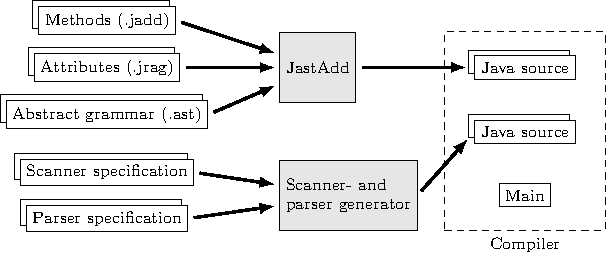
\includegraphics{jastadd/generation-process.pdf}
\caption{A typical compiler generation process using JastAdd.}
\label{JA-GenerationProcess}
\end{center}
\end{figure}

For the Oberon-0 compiler, the artifacts are specified in different directories: \texttt{A1}, \texttt{A2a}, \texttt{A2b}, \texttt{A3}, and \texttt{A4}. Within each directory, there are specification files for scanner, parser, abstract grammar, attributes, and methods. Typically, there are several attributes and methods files for different subproblems, e.g., name analysis, type checking, etc. Each artifact (except for \texttt{A1}) extends one or more previous artifacts, and its directory contains the specification files for that extension only. To build an artifact, an \emph{Ant} build file is used that simply lists all the relevant specification directories. This allows reuse of all the specification files from the previous artifacts, and only the build script and the main program need to be written specifically for the artifact. An explicit import mechanism would have been preferable to simply listing directories in the build script, but this is currently lacking in JastAdd. Figure~\ref{JA-ArtifactsOverview} shows all the specification files in the different artifact directories, their size, and how they depend on each other.

\begin{figure}[h]
\begin{center}
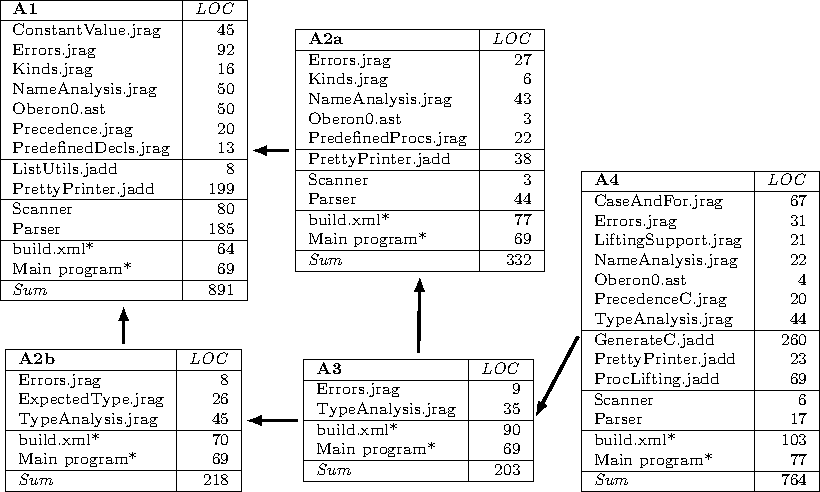
\includegraphics{jastadd/artifacts-overview.pdf}
\caption{An overview of modules in artifacts and how they extend each other. Arrow means extension and * means that the file is not reused.}
\label{JA-ArtifactsOverview}
\end{center}
\end{figure}

Figure~\ref{JA-AbsGram} shows some of the abstract grammar classes defined in the \texttt{A1} artifact. Abstract grammars are typically extended by adding new subclasses. For example, to extend Oberon-0 with procedures, a new class \texttt{Procedure} is defined in the \texttt{A2a} artifact, as a subclass of \texttt{Decl}.

\begin{figure}[h]\footnotesize
\begin{jastaddcode}
Module ::= <StartId> Decl* Block <EndId>; // The root class
abstract Decl;                     // Superclass for declarations
abstract Stmt;                     // Superclass for statements
Block : Stmt ::= Stmt*;            // Subclass for blocks
abstract Expr;                     // Superclass for expressions
abstract Access : Expr;            // Subclass for accesses
SimpleAccess : Access ::= IdUse;   // Subclass for access to simple var
IdDecl ::= <ID>;                   // Declared identifier
IdUse ::= <ID>;                    // Use of a declared identifier
...
\end{jastaddcode}
\vspace{-15pt}
\caption{Some of the abstract grammar classes defined in \texttt{A1/Oberon0.ast}. Tokens are enclosed in angle brackets. Lists are indicated by the Kleene star.}
\label{JA-AbsGram}
\end{figure}

Unfortunately, JFlex and Beaver do not support modularized specifications. For JFlex, we currently use a workaround by splitting the specification into several files, and concatenating them in different ways in the different build scripts. For Beaver, we use a preprocessor, called \emph{JastAddParser}, that has a specification similar to Beaver's, but where different productions can be specified in different files. This allows us to achieve the desired modularization also for the parsing, although in a somewhat clumsy way.


%
% Name analysis
%
\subsection{Name analysis}
\label{JA-NameAnalysis}
The task of name analysis is to bind an identifier usage to the corresponding declaration,
taking into account the language's scope rules. For Oberon-0, we represent identifier usages by the class \texttt{IdUse}, declarations by \texttt{IdDecl}, and bindings by a reference attribute \texttt{decl} in \texttt{IdUse}. The \texttt{decl }attribute is defined using an inherited parameterized attribute \texttt{lookup(String)}. This attribute is defined in some parent of the \texttt{IdUse}, typically in a procedure or a module, and will find the appropriate \texttt{IdDecl} node, given the identifier name as argument. This design makes it unnecessary to construct explicit symbol tables or environment data structures: we can instead use the AST itself as this structure. The Figure~\ref{JA-DeclNameAnalysis} shows part of the name analysis for artifact \texttt{A1}, and an example is shown in Figure~\ref{JA-UseDecl}. The equation in \texttt{Module} makes use of two other parameterized attributes, \texttt{localDeclLookup} and \texttt{localPredefinedLookup}, to delegate the search to the local declarations and the predefined declarations, respectively.

\begin{figure}
\begin{jastaddcode}
syn IdDecl IdUse.decl() = lookup(getID());
inh IdDecl IdUse.lookup(String name);
eq Module.getBlock().lookup(String name) {
    IdDecl decl = localDeclLookup(getNumDecl()-1, name);
    if (decl == null) decl = localPredefinedLookup(name);
    return decl;
}
\end{jastaddcode}
\vspace{-15pt}
\caption{Part of the name analysis for Oberon-0}
\label{JA-DeclNameAnalysis}
\end{figure}

\begin{figure}[h]
\begin{center}
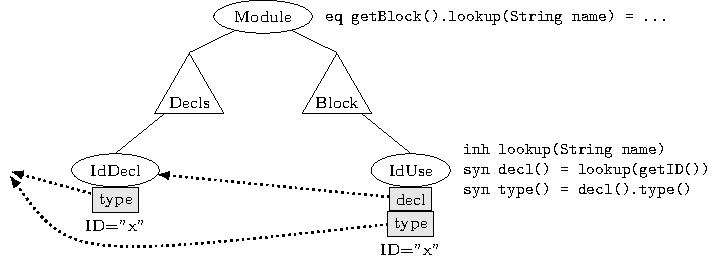
\includegraphics{jastadd/use-decl.pdf}
\caption{An AST illustrating how uses are bound to declarations, with the \texttt{decl} attribute. 
	Ellipses are AST nodes. Triangles are subtrees. Rectangles are attributes. 
	Solid lines are child/parent links. Dotted lines are reference values.}
\label{JA-UseDecl}
\end{center}
\end{figure}

In artifact \texttt{A2a}, procedures are added, and the name analysis needs to be extended with support for nested scopes. The Figure~\ref{JA-ProcNameAnalysis} shows how this is handled: The abstract syntax is extended with classes for \texttt{Procedure} and \texttt{ProcedureCallStmt}, and an equation for \texttt{lookup} is added in \texttt{Procedure}. The equation first searches locally among parameters and declarations in the procedure, and if no match is found there, the search is delegated to the context of the \texttt{Procedure}, using the l\texttt{ookup} attribute of the \texttt{Procedure} itself. This attribute is also declared in the figure, and will be defined by a parent \texttt{Module} or \texttt{Procedure} node, depending on the structure of the program.

\begin{figure}
\begin{jastaddcode}
Procedure : Decl ::= IdDecl ParDecl* Decl* Block <EndId>;
ProcedureCallStmt : Stmt ::= IdUse Expr*;

eq Procedure.getDecl(int index).lookup(String name) {
	IdDecl decl = localParLookup(name);
	if (decl == null) decl = localDeclLookup(index, name);
	if (decl == null) decl = lookup(name);
	return decl;
}
inh IdDecl Procedure.lookup(String name);
\end{jastaddcode}
\vspace{-15pt}
\caption{Extending Oberon-0 with procedures and nested name analysis} 
\label{JA-ProcNameAnalysis}
\end{figure}

In Oberon-0, constants, types, variables and procedures all use the same namespace. 
We can therefore use \texttt{IdDecl} and \texttt{IdUse} for all these
constructs, and share the definition of the \texttt{lookup} attribute between them.
To handle the \emph{declare before use} policy that applies within a declaration part, for example to look up type names, an additional parameter is used for \texttt{localDeclLookup}, to search only up to a certain point in the declaration list.

Oberon-0 contains a number of predefined declarations, e.g., the types \texttt{INTEGER} and \texttt{BOOLEAN}. In order to allow these to be handled in the same way as user-defined declarations, they are also represented in the AST. This is done using the NTA \texttt{predefinedDecls} in \texttt{Module}. A \emph{non-terminal attribute} (NTA) is both an attribute and an AST subtree at the same time, and is also called a \emph{higher-order attribute}~\cite{vogt89pldi}. The subtree of an NTA is created as the result of evaluating its defining equation. Figure~\ref{JA-PredefinedDecls} shows how a variable declaration uses the predefined type \texttt{INTEGER}, and how the \texttt{IdUse} of its type is bound to the \texttt{IdDecl} declaring \texttt{INTEGER} in the NTA.


%
% Type checking
%
\subsection{Type checking}
\label{JA-TypeChecking}

To typecheck an Oberon-0 expression, we compare its actual type with the type expected by its context. This is captured in two attributes: the inherited attribute \texttt{expectedType} and the synthesized attribute \texttt{type}. For example, for an assignment, the expected type of the right-hand side expression is the same as the type of the left-hand side variable, see Figure~\ref{JA-ExpectedType}.

\begin{figure}[h]
\begin{jastaddcode}
inh Type Expr.expectedType();

eq AssignmentStmt.getExpr().expectedType() = getAccess().type();
eq IfStmt.getExpr().expectedType() = module().boolType();
...
\end{jastaddcode}
\vspace{-15pt}
\caption{Definition of the inherited attribute \texttt{expectedType}}
\label{JA-ExpectedType}
\end{figure}

Type-checking errors, and other compile-time errors, are collected into a set-valued attribute \texttt{errors} in the \texttt{Module} node (the root of the AST). The \texttt{errors} attribute is a \emph{collection attribute}  \cite{boyland98cc,magnusson09ase} whose value is defined by \emph{contribution} rules, one for each possible compile-time error. 
Figure~\ref{JA-TypeErrors} shows how type-checking errors are collected, simply by contributing an error object when the actual and expected types are not compatible. Here, \texttt{error(String s)} is a method returning a fresh error object, \texttt{compatibleWith(Type~t)} is a parameterized synthesized attribute for comparing types, and \texttt{module()} is an inherited attribute returning the \texttt{Module} root node.

\begin{figure}[h]
\begin{jastaddcode}
Expr contributes error("Type error ...")
	when !type().compatibleWith(expectedType())
	to Module.errors() for module();
\end{jastaddcode}
\vspace{-15pt}
\caption{Collection of type checking errors}
\label{JA-TypeErrors}
\end{figure}

The synthesized attribute \texttt{type} is defined for the different kinds of expressions. For operators, the value is typically a predefined type, like \texttt{INTEGER} or \texttt{BOOLEAN}. The type of a variable or constant access is normally the type of its declaration. However, we also need to take into account that the declaration may be missing, or it may be a circularly defined constant, like \texttt{CONST c = c}. In these cases, we represent the type by an object \texttt{unknownType}, see Figure~\ref{JA-SimpleIdUse}. 

\begin{figure}
\begin{jastaddcode}
syn Type Expr.type();
eq RelationExpr.type() = module().boolType();
eq ArithmeticBinExpr.type() = module().integerType();
...
eq SimpleAccess.type() = getIdUse().type();

syn Type IdUse.type() {
	if (decl() == null || isCircular()) 
		return module().unknownType();
	return decl().type();
}
\end{jastaddcode}
\vspace{-15pt}
\caption{Definition of the synthesized attribute \texttt{type}}
\label{JA-SimpleIdUse}
\end{figure}

To resolve the type of a declaration, each \texttt{IdDecl} has an inherited attribute \texttt{type}. (Figure~\ref{JA-SimpleIdUse} showed an example use of the attribute.) Often, the type in a declaration is itself a use of a type declared elsewhere. It is then represented by a \texttt{TypeUse} node that contains an \texttt{IdUse} node which handles the name binding to the (type) declaration, just like for variables and constants. Figure~\ref{JA-PredefinedDecls} shows an example for the variable declaration \texttt{VAR~x~:~INTEGER;} The actual type of \texttt{x} is found by following the \texttt{decl} reference attribute in the type use. In this case, the type is located among the predefined declarations, in the NTA in the AST root.

\begin{figure}
\begin{center}
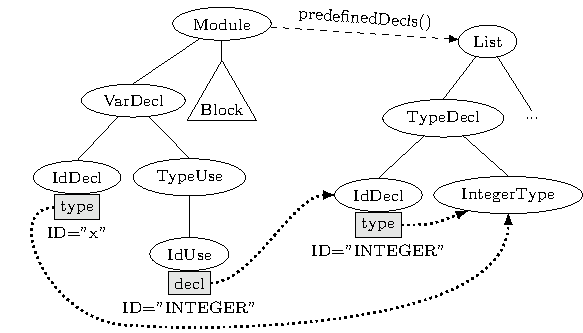
\includegraphics{jastadd/predefined-decls.pdf}
\caption{Shows binding of a type use, for \texttt{VAR x:INTEGER}, where \texttt{INTEGER} is a predefined type. Dashed lines are NTAs (e.g. \texttt{predefinedDecls}).}
\label{JA-PredefinedDecls}
\end{center}
\end{figure}


%
% Source-to-source transformation
%
\subsection{Source-to-source transformation}
Our implementation includes two kinds of source-to-source transformations: 1) procedure lifting in order to simplify generation of C code (since C functions cannot be nested), and 2) translating a larger language to a syntactically smaller core language, also to simplify code generation. 

Procedure lifting is implemented by generating a new AST where declarations of procedures, types and constants are moved to the top level. This is implemented as a method that traverses the original AST to build the new one, and uses attributes to decide what to build. For example, to generate new identifiers, the path from the root down to a declaration is used, and is captured by an inherited attribute \texttt{astPath} in \texttt{IdDecl}. The transformation is idempotent: applying the transformation more than once yields the same result. This is accomplished by using attributes to check if the original AST includes only top-level constructs.

To translate from a larger to a syntactically smaller language, NTAs are used. An example is translating \texttt{CASE} to \texttt{IF}.
This is done by defining an NTA \texttt{ifEquivalent} in \texttt{CaseStmt}. This simplifies code generation, since code can be generated for \texttt{CaseStmt} simply by delegating to the NTA. However, the NTA is only used for code generation: all compile-time error checking is still done directly in the original \texttt{CaseStmt}, in order to give error messages in terms of the original construct. The same technique is used to translate \texttt{FOR} to \texttt{WHILE}. Here, construction of the NTA is actually not simpler than just generating the code directly, but will pay off if several code generators for different targets are implemented.

%
% Code generation
%
\subsection{Code generation}
Generation of C code is implemented with a method \texttt{generateC}
that traverses the AST, making use of attributes to generate the correct code.
The code generation is similar to pretty printing, but needs to handle some additional things, like name collision with C's keywords, and that type declarations in C are structured in a somewhat different way. Parentheses are not stored in the AST, but are added during code generation and pretty printing, using attributes to encode the precedence rules.

To generate code for \texttt{CASE} and \texttt{FOR} is easy, it just amounts to delegating the work to the NTA. For example, the \texttt{ForStmt} class, delegates the code generation to its NTA \texttt{whileEquivalent}: 

\begin{jastaddcode}
public void ForStmt.generateC(StringBuilder sb, int indent) {
	whileEquivalent().generateC(sb, indent);
}
\end{jastaddcode}


%
%  Concluding observations
%
\subsection{Concluding observations}
\emph{Ease of use.} 
The main characteristic of JastAdd is its declarative specification technique that makes use of and blends with object-oriented programming: the AST is represented by an object-oriented model that arguably a normal OOP programmer would have constructed, but replaces imperative compiler phases with declarative computations in the form of attributes and equations.

In constructing the Oberon-0 compiler, we have reused a number of design ideas from earlier JastAdd compilers. These include:
\begin{itemize}
  \item Synthesized reference attributes, typically called \texttt{decl}, and inherited parameterized attributes, typically called \texttt{lookup}, for name analysis.
  \item Parameterized attributes that use double dispatch (calling another attribute) for comparing types~\cite{ekman07oopsla}.
  \item Collection attributes for collecting compile-time error messages.
  \item Non-terminal attributes for representing predefined declarations.
  \item Non-terminal attributes for representing new language constructs in terms of existing ones, in order to simplify code generation.
  \item Imperative methods that access attributes in order to implement pretty-printing and code generation.
\end{itemize}
We consider these design choices to be useful for most compiler implementations in JastAdd, and to demonstrate best practices in using the system.

\emph{Modularity.}
The declarative approach, together with the OO AST model and the use of AspectJ inter-type declarations, gives very strong support for modularization and extensibility. This is demonstrated by the Oberon-0 artifacts where all code except for the main programs and build files were reused in extensions. However, it should be noted that while extensions are often easy to add, it is not always completely straightforward. Sometimes, the base modules can be refactored to better support extension. We encountered one such example when arrays and records were to be added in artifact \texttt{A4}. Originally, artifact \texttt{A1} modeled variable accesses using a class \texttt{Access} that was a subclass to \texttt{Expr} and had an \texttt{IdUse} as its child:

\begin{jastaddcode}
Access : Expr ::= IdUse;
\end{jastaddcode}

However, when more complex accesses were added, like \texttt{ArrayElementAccess} and \texttt{RecordFieldAccess}, we needed them to subclass a more abstract \texttt{Access} class, since they had a different child structure. This was accomplished by refactoring \texttt{A1}, splitting the class \texttt{Access} into two: an abstract class \texttt{Access} and a subclass \texttt{SimpleAccess}, see Figure~\ref{JA-AbsGram}.

\emph{Analysis of specifications.}
JastAdd supports certain analysis of specifications: Static checks include checking that each attribute will have a defining equation for any possible AST. Dynamic checks include detection of cyclic evaluation (for attributes not declared as circular). We believe that the error messages are of reasonable quality. However, there is also room for improvement in several ways: The attribute equations are written in Java, and compile-time errors in them are not checked until compiling the generated Java code. While these errors are reasonably simple to map back to the equations in the JastAdd source code, it would have been better to get them directly in terms of that code. Furthermore, side effects are not allowed in the equations, but this is not checked, and may give rise to errors that are difficult to debug. This is something we would like to improve, for example by including an analysis similar to the the one proposed in the JPure system~\cite{pearce11cc}.

\emph{Performance.} JastAdd gives compilers of reasonable performance, as exemplified by the JastAdd Extensible Java compiler that performs within a factor of three in comparison to the Java reference compiler javac~\cite{ekman07oopsla}. 

To conclude, we think that the Oberon-0 implementation demonstrates well the language modularization capabilities of JastAdd, as well as many best practices for using the tool.

\section{Rascal, a DSL for meta-programming}

%\def\rascal{\textsc{Rascal}\xspace}
\def\oberon{\textsc{Oberon-0}\xspace}

% todo: use rascal.sty
\def\rcode#1{\texttt{#1}}

\subsection{Introduction}

\noindent \Rascal is a domain-specific language for
meta-programming. It has been designed to deal with software languages
in the broadest sense of the word. Its application areas include the
development of DSLs, reverse engineering and reengineering of (legacy)
software systems and software repository mining. \Rascal features
powerful domain-specific language constructs to make meta programming
more effective:
\begin{itemize}
\item Integrated syntax definition: context-free grammars can be
  declared as part of ordinary \Rascal code; the parse trees defined
  by such grammars are first-class values, and non-terminals are
  first-class types.
\item Built-in data types: apart from the standard data types (int,
  bool, string etc.), \Rascal supports sets, relations, maps, lists,
  algebraic data types (ADTs), parse trees, and source
  locations. Every value in Rascal can be used in pattern
  matching. This includes concrete syntax trees produced by \Rascal's
  grammar.
\item Constructs for analysis and transformation: sets, relations,
  maps and lists can be used in comprehensions. The visit-statements
  allows for structur-shy traversal and rewriting of abstract or
  concrete syntax trees.
\end{itemize}
\Rascal is \textit{programming language}; it eschews implicit
features. The language design is informed by learnability and
debuggability considerations. This means there is little ``magic'' in
\Rascal. For instance, control-flow is completely straightforward,
unlike, for instance, in languages based on attribute evaluation or
term rewriting~\cite{...}. \Rascal adheres to the
what-you-see-is-what-you-get (WYSIWYG) principle.

\subsubsection{Overview of the \Rascal \oberon implementation}

\noindent \Rascal allows computer languages to be implemented in a modular
fashion, through the simultaneous extension of syntax definition
(grammars), algebraic data types (ADTs) and functions operating on
data conforming to these data types. The \oberon implementation
consists of four layers corresponding to each language level. An
overview of the architecture is shown in Table~\ref{TBL:rascalArch}.

\begin{table}
\begin{center}\small
\begin{tabular}{|l||l|l|l|}\hline
   &  Syntax & Data Type & Function \\\hline\hline
L1 &  \textbf{grammar} & \textbf{AST}, \textbf{scope} & 
\textbf{bind}, \textbf{check}, \textbf{format}, \textbf{compile} \\\hline 
L2 & +grammar & +AST & +bind, +check, +format, \textbf{desugar} \\\hline
L3 & +grammar & +AST, +scope & +bind, +check, +format, +compile, \textbf{lift} \\\hline
L4 & +grammar & +AST & +bind, +check, +format, +compile \\\hline
\end{tabular}
\end{center}
\caption{Layered architecture of the \Rascal \oberon implementation;
  ``+'' indicates extension, \textbf{bold} indicates introduction.\label{TBL:rascalArch}}
\end{table}

The table show three columns, corresponding to syntax definition,
(algebraic) data types and functions. Each row corresponds to a
language level. Level L1 represents the base case: all relevant
syntax, data types and functions are introduced here. In the
subsequent levels any of these types and functions may have to be
extended. For instance, in L2, where the FOR and CASE statements are
introduced, the grammar and AST definition of L1 are extended with new
alternatives to deal with these constructs. Similarly, the functions
bind, check and format are extended. However, the compile function is
not extended; instead FOR and CASE statements are desugared to L1
constructs. Note also that the scope data type used during name
analysis is reused as is. This data type only needs to be extended
when procedures are introduced in L3. In L3 we introduce a lift
function to move nested procedures to top level.

Extension in \Rascal works through the \texttt{extend} construct. This
constructs works similar to module import, except that it allows the
extension of recursively defined abstractions, in this case ADTs and
functions. This leads to a mechanism similar to inheritance in
object-oriented languages~\cite{Cook?}.  For grammars and ADTs the
definitions of the extended module and the extending module are simply
merged. Function extension, on the other hand, depends on a particular
style of writing \Rascal functions, in a way similar to term rewriting
rules. An example may illustrate the approach. For instance the
following rule implements the \texttt{check} function for
type-checking WHILE statements:
\begin{quote}
\begin{rascal}
set[Message] check(whileDo(c, b)) =
                 checkCond(c) + checkBody(b);
\end{rascal}
\end{quote}
It looks like an ordinary \Rascal function definition except that it
uses ``= $\langle$\textit{Expression}$\rangle$'' instead of a regular
function body using $\{\}$. Moreover, the function uses pattern
matching in its signature to dispatch on the WHILE AST constructor;
this style of function definition hence is called
\textit{pattern-based dispatch}.  The complete implementation of the
\texttt{check} function consists of multiple such rules, one for each
AST constructor. Such rules may be distributed over different modules
to obtain extensibility. For instance, in L3 where procedure
definitions and procedure calls are introduced, the \texttt{check}
function is extended by adding an implementation rule dispatching on
the AST constructor for procedure calls. In the \oberon implementation
\texttt{bind}, \texttt{check}, \texttt{format}, and \texttt{compile}
are modularized using pattern-based dispatch.

For syntax and abstract syntax the mechanism is similar. In higher
layers (i.e., L2, L3, and L4), extension modules add alternatives to
both grammars and ADTs. Note that for grammars this requires a general
parsing algorithm, since only the full class of context-free languages
is closed under union~\cite{?}. In L3 this mechanism is used to extend
the scope data type to deal with nested scopes. In L1 this data type
is defined as follows:
\begin{quote}
\begin{rascal}
data NEnv = scope(map[Ident, Decl] env);
\end{rascal}
\end{quote}
In other words the the name environment consists of a plain map from
identifiers to declarations. By wrapping this map in an ADT
constructor, the type \texttt{NEnv} becomes extensible. In L3 it is
extended as follows:
\begin{quote}
\begin{rascal}
data NEnv = nest(map[Ident, Decl] env, NEnv parent);
\end{rascal}
\end{quote}
The new alternative (\texttt{nest}) also consists of a
name-declaration map, but also has an additional parent
\texttt{NEnv}. 

\subsection{Scanning and parsing}

\noindent \Rascal's syntax definitions are backed by a scannerless, general
parsing algorithm based GLL~\cite{JohnstoneScott11}. Scannerless
parsing solves the problem of modular lexical syntax. To deal with
(lexical) ambiguities, \Rascal has built-in support for longest-match
and keyword reservation. Consequently, each language level may
introduce additional reserved keywords, that are not reserved in
previous levels. For instance, the ``FOR'' keyword, introduced in L2,
is not reserved in L1

Grammars are annotated with constructor names to obtain automatic
mapping of parse trees to ASTs. The \Rascal standard library function,
\texttt{implode}, converts and concrete syntax tree into an AST, given
an ADT definition of the abstract syntax. Implode uses the
\textit{reified ADT} as a recipe. Reified types are reflective value
representations of \Rascal types. The information in the reified type
is used by implode to decide how an concrete tree must be mapped to an
AST. For instance, some lexical parse tree nodes are mapped to
(native) integers if this is dictated by the abstract syntax ADT.

The statement syntax of \oberon L1 is defined as follows:
\begin{quote}
\begin{rascal}
syntax Statement 
  = assign: Ident ":=" Expression
  | ifThen: "IF" Expression "THEN" 
               {Statement ";"}+  ElsIfPart* ElsePart? "END"
  | whileDo: "WHILE" Expression "DO" {Statement ";"}+ "END"
  | skip: ;
\end{rascal}
\end{quote}
Each alternative is labeled with a constructor name that corresponds
to a constructor in the abstract syntax, which (for statements) is
defined as follows:
\begin{quote}
\begin{rascal}
data Statement 
  = assign(Ident var, Expression exp)
  | ifThen(Expression condition, list[Statement] body, 
       list[ElsIf] elseIfs, list[Statement] elsePart)
  | whileDo(Expression condition, list[Statement] body)
  | skip()
  ;
\end{rascal}
\end{quote}
In the abstract syntax ordinary \Rascal lists are used for regular
operators.  The \Rascal parser annotates parse trees with source
locations (a native datatype in Rascal). The implode propagates these
locations to the AST so that meaningful error messages can be given
during later processing.

Scannerless means that there is no separate tokenization phase: both
lexical and context-free syntax are described using the same grammar
formalism. This makes it, for instance, trivially easy to support
\oberon's nested comments:
\begin{quote}
\begin{rascal}
lexical Comment = "(*" CommentElt* "*)" ;
lexical CommentElt = CommentChar+ | Comment ;
lexical CommentChar = ![*(] | [*] !>> [)] | [(] !>> [*];
\end{rascal}
\end{quote}
In essence, this is just context-free syntax, except the
\texttt{lexical} keyword indicates that no layout is allowed between
symbols. The CommentChar non-terminal captures all characters except
``*'' and ``('', and uses follow restrictions (``\texttt{!>>}'') to
allow both ``*'' and ``('' if they are not followed by ``)'' and ``*''
respectively.

\subsubsection{Formatting}

\noindent Formatting in \Rascal consists of mapping (abstract) syntax
trees to Box constructs~\cite{Box}. The resulting Box expressions
describes how elements should be layed out, e.g., horizontally,
vertically, indented or aligned, which font-style to use, and how
adjacent elements should be spaced relative to one another.

As an example, consider the formatting of the WHILE statement:
\begin{quote}
\begin{rascal}
Box stat2box(whileDo(c, b)) = V([
   H([KW(L("WHILE")), exp2box(c), KW(L("DO"))])[@hs=1],
      I([V(hsepList(b, ";", stat2box))]),
   KW(L("END"))
]);  
\end{rascal} 
\end{quote}
Again this function uses pattern-based dispatch to match the AST
constructor for WHILE statements. The result of the function is a Box
expression (which is just an ADT in \Rascal). The result dictates that
the WHILE and DO are both keywords (KW), and the condition \irascal{c}
is formatted using the function \irascal{exp2box}. All three sub-boxes
should be laid out horizontally (H). Finally, the spacing between the
elements should be 1, as indicated by the annotation \texttt{@hs=1}.
The body \irascal{b} of the WHILE statement should be indented one
level (I), and the statements should be placed vertically. The helper
function \irascal{hsepList} is used to correctly combine separated
lists where the separator (``;'') should be horizontally combined with
an element; it is parameterized by the a function to convert each
element of the list to a Box expression (i.c., \irascal{stat2box}).
Finally, the three sub-boxes are wrapped in a V box so that the
header, body and END keyword are placed vertically.

A common problem with pretty-printing is the (re)insertion of
parentheses in binary expressions according to the precedence and
associativity rules of the grammar. In \Rascal this can be solved
using reified types. Above, we described how \irascal{implode} used
the reified type of the abstract syntax ADT to guide the mapping of
parse trees to ASTs. In this case we proceed the other way around: we
use the reified type of the \textit{grammar} to obtain precedence and
associativity information. Since all non-terminals are first-class
types in \Rascal, obtaining the reified type of a non-terminal gives
us the complete grammar. 

To illustrate how this works, consider the following formatting rule
for multiplication expressions:
\begin{quote}
\begin{rascal}
Box exp2box(p:mul(lhs, rhs)) = 
    H([exp2box(p, lhs), L("*"), exp2box(p, rhs)])[@hs=1];
\end{rascal}
\end{quote}
This rule lays out expressions horizontally. But instead of calling
directly the unary function \irascal{exp2box} on \irascal{lhs} and
\irascal{rhs}, there is an intermediate call to \irascal{exp2box} with
two arguments; in both cases the first argument is \irascal{p} which
is bound to the current expression using \texttt{p:}. This parent
expression is used to decide whether to insert parentheses or not:
\begin{quote}
\begin{rascal}
Box exp2box(Expression parent, Expression kid) =
    parens(PRIOS, parent, kid, exp2box(kid), parenizer);

Box parenizer(Box box) = H([L("("), box, L(")")])[@hs=0];
\end{rascal}
\end{quote}
In this example, the global constant \irascal{PRIOS} contains
the precedence information obtained from the grammar. The
\irascal{parens} function checks if the occurence of \irascal{kid}
directly below \irascal{parent} requires parentheses, and if so, calls
\irascal{parenizer} on the Box expression resulting from
\irascal{exp2box(kid}). The function \irascal{parenizer} simply
horizontally wraps the argument with parentheses.


\subsection{Name analysis}

\noindent Name analysis consists of a traversal of the AST that does
two things at the same time:
\begin{enumerate}
\item Annotate use sites of variables, types and constants with the
  their declarations.
\item Maintain a set of error messages, indicating problems such as
  undeclared identifiers. 
\end{enumerate}
These two concerns are implemented in functions \irascal{bindModule},
\irascal{bindStat}, \irascal{bindExp} etc. They carry around a
\irascal{NEnv} environment which contains the names that are currently
in scope (cf. above for its definition). If an identifier is
encountered, it is looked up in the environment and, if found, the
identifier is annotated using a \Rascal annotation representing the
declaration.

In order to both annotate ASTs and return a set of error messages the
\irascal{bind} family of functions returns a tuple containing an AST
node and a set of error messsages. This type is defined as the
following \Rascal alias:
\begin{quote}
\begin{rascal}
alias Bound[&T] = tuple[&T ast, set[Message] errs];
\end{rascal}
\end{quote}

As an example, consider the binding of the IF-statement, which is
shown below:
\begin{quote}\small
\begin{rascal}
Bound[Statement] bindStat(s:ifThen(c, b, eis, e), 
                     NEnv nenv, set[Message] errs) {
    <s.condition, errs> = bindExp(c, nenv, errs);
    <s.body, errs> = bindStats(b, nenv, errs);
    s.elseIfs = for (ei <- eis) {
      <ei.condition, errs> = bindExp(ei.condition, nenv, errs);
      <ei.body, errs> = bindStats(ei.body, nenv, errs);
      append ei;
    }
    <s.elsePart, errs> = bindStats(e, nenv, errs);
    return <s, errs>;
}
\end{rascal}
\end{quote}
The function heavily uses \Rascal's destructuring assignment to
simultaneously replace parts of the AST and update the \irascal{errs}
variable. For instance, the first statements invokes \irascal{bindExp}
to bind the condition of the IF-statement; the resulting annotated
expression is inserted in place of the original condition
(\irascal{s.condition}). The reason for this idiom is that it is
impossible to simply rebuild the tree, because then the source
location annotations would be lost. The for-loop folds over the list
of ELSIF's while at the same time (possibly) updating the set
\irascal{errs}. The final result is the annotated IF-node
(\irascal{s}) together with the \irascal{errs}.

The annotation of identifiers is implemented using the following
function: 
\begin{quote}\small
\begin{rascal}
Bound[Ident] bindId(Ident x, NEnv nenv, set[Message] errs) {
  if (isVisible(nenv, x))
    return <x[@decl=getDef(nenv, x)], errs>;  
  if (x.name in {"TRUE", "FALSE"})
    return <x[@decl=trueOrFalse(x.name == "TRUE")], errs>;
  return <x, errs + { undefIdErr(x@location) }>;
}
\end{rascal}
\end{quote}
This function checks the name environment (\irascal{nenv}) if the
identifier \irascal{x} is currently visible. If so, then the
\irascal{x} is annotated with its definition
(\texttt{x[@decl=...]}). Otherwise, if \irascal{x} represents that
boolean constants TRUE or FALSE, it is annotated accordingly. If none
of the above holds, the identifier is undeclared and an error is
produced, containing the source location of \irascal{x}.

\subsection{Type checking}

\noindent Similar to the name-analysis, type checking is an abstract
interpretation of the AST, computing a set of error messages. Unlike
in the case of name-analysis, however, the AST is not annotated with
further information; all required annotations are assumed to be set
during name analysis. This simplifies type checking considerably,
since all required information is local to a certain AST node.

As an example, consider the following code to check procedure calls:
\begin{quote}
\begin{rascal}
set[Message] check(s:call(f, as)) {
  if (!(f@decl is proc)) 
    return { notAProcErr(f@location) };
  if (size(as) != arity(f@decl.formals)) 
    return { argNumErr(s@location) };
  errs = {}; i = 0;
  for (frm <- f@decl.formals, n <- frm.names) {
    errs += checkFormal(n, as[i], frm.hasVar);
    i += 1;
  }
  return ( errs | it + check(a) | a <- as);
}
\end{rascal}
\end{quote}
First the declaration of the called procedure is retrieved in order to
check whether \irascal{f} actually represents a procedure. If not, an
error is returned. Second, list of formal parameters is obtained from
the \irascal{decl} annotations and the arity of the procedure is
checked. Third, now we can assume that the number of actual parameters
is correct, each argument is checked against its corresponding formal
parameter using \irascal{checkFormal}. Finally each actual parameter
is checked individually for type errors. The result of this function
is the union of the set of errors collected in the for-loop and the
union of all sets of errors returned for each actual argument.

\subsection{Source-to-source transformation}

\noindent \Rascal features builtin support for structure-shy traversal
of data structures using the \rcode{visit} statement. Visit works like
a traditional case statement, only cases are matched at arbitrary
depth in a data structure. There are 6 builtin strategies to control
the traversal order. Visited nodes maybe replaced, thereby rewriting
the tree, similar to traversal rules in \cite{ASF+SDF} and rewrite
strategies in \cite{Stratego}.


The desugaring of FOR-loops and CASE-statements both heavily depend on
the visit-statement. For instance, the desugaring of the
for-statements introduced in L2 is shown in
Listing~\cite{LST:for2while}. The function \irascal{for2while} visits
a list of statements. First FOR-loops without a BY-clause are
normalized to have a BY-clause of 1 (\irascal{nat(1)}). Second, if a
BY-clause uses a symbolic constant, it is replaced with the integer
the constant evaluates to. Then, in the thrid and fourth case,
FOR-loops are substituted for equivalent L1 \oberon nodes. Since a
single FOR-loop is desugared to a sequence of statements, we use a
temporary AST constructor, \irascal{begin}, to allow inserting
multiple statements in place of one. The \irascal{begin} nodes are
spliced into their surrounding context in a later phase. Note that the
use of the \rcode{innermost} keyword ensures that FOR-loops are first
normalized and only after that will be eventually desugared.

\begin{listing}[t]
\begin{quote}
\begin{rascal}
public list[Statement] for2while(list[Statement] stats) {
 return innermost visit (stats) {
  case forDo(n, f, t, [], b) => forDo(n, f, t, [nat(1)], b)
  case forDo(n, f, t, [lookup(x)], b) => forDo(n, f, t, [c], b)
           when x@decl is const, c:nat(_) := eval(x)
  case forDo(n, f, t, [nat(x)], b) => 
           begin([assign(n, f), whileDo(leq(lookup(n), t), 
              [b, assign(n, add(lookup(n), nat(x)))])]) 
  case forDo(n, f, t, [neg(nat(x))], b) => 
           begin([assign(n, f), whileDo(geq(lookup(n), t), 
              [b, assign(n, sub(lookup(n), nat(x)))])]) 
 }
}
\end{rascal}
\end{quote}
\caption{Desugaring \oberon FOR-loops to WHILE-loops in
  \Rascal\label{LST:for2while}} 
\end{listing}

The desugaring of the CASE-statement to nested IF-statements is
implemented in a similar way.


\subsection{Code generation}


\subsubsection{Unique names}

\noindent To ensure that there will be no name collisions after
procedures, types and constants are lifted, identifiers referring to
such entities are first ``uniqified''. For names in declarations, the
source location's offset is used to make the name unique\footnote{This
  trivially gives uniqueness, since no two identifiers can occupy the
  same offset in a source file.}. To rename use sites of
identifiers, the location of its declaration is obtained from the
name-binding \irascal{decl} annotation.

The \irascal{rename} function is implementation is shown below:
\begin{quote}
\begin{rascal}
Module rename(Module m, NEnv global) {
  return visit (m) {
    case constDecl(x, e) => constDecl(prime(x), e)
    case typeDecl(x, t) => typeDecl(prime(x), t)
    case proc(x, fs, ds, b, f2) => proc(prime(x), fs, ds, b, f2)
    case call(x, as) => call(prime(x, l)
       when proc(l, _) := x@decl, !isDefined(global, x)
    case user(x) => user(prime(x, l))
      when \type(l, _) := x@decl
    case lookup(x) => Lookup(prime(x, l))
      when const(l, _) := x@decl
  };
}
\end{rascal}
\end{quote}
The \irascal{rename} performs a single traversal over the AST and
inserts \irascal{prime}d names into declarations and use sites. For
the use sites the locations of and identifiers declaration is used.

\subsubsection{Lifting procedures}

\noindent Standard C does not support nested functions. To simplify
the code generation, \oberon procedures are first lifted to the
top-level. Below is the function that lifts nested procedures and
produces a flat list of procedure declarations:
\begin{quote}
\begin{rascal}
public list[Procedure] liftProc(Procedure proc) {
  newProcs = ( [] | it + liftProc(p) | p <- proc.decls.procs );
  proc.decls.procs = [];
  return newProcs + [proc];
}
\end{rascal}
\end{quote}
...
A similar procedure is applied for type and constant declarations. 

\subsubsection{Generating C-code}

\noindent Although it would have been possible to define an abstract
syntax for C and then use \Rascal's Box formatting to obtain a textual
representation suitable for compiling to machine code, we have instead
opted for a simpler, more pragmatic approach using string
templates. In \Rascal string literals can be interpolated with
expressions, conditional statements (if) and loops (for, while,
do-while). This makes string templates very convenient for generating
code. Moreover, using the explicit margin markers (single quote '),
such templates are convenient to write and the result will be
automatically indented. For instance, consider the code to generate
code for WHILE loops and IF statements a C while-loop:
\begin{quote}
\begin{rascal}
str stat2c(whileDo(c, b)) = "while (<exp2c(c)>) {
                            '  <stats2c(b)>
                            '}";

str stat2c(ifThen(c, b, ei, ep)) = 
                            "if (<exp2c(c)>) {
                            '  <stats2c(b)>
                            '}<for (<ec, eb> <- ei) {>
                            'else if (<exp2c(ec)>) {
                            '  <stats2c(eb)>
                            '}<}>
                            '<if (ep != []) {>
                            'else {
                            '  <stats2c(ep)>
                            '}<}>";
\end{rascal}
\end{quote}
In both string templates the statements within statement blocks will
be indented relative to the margin. All whitespace to the left of the
margin is discarded.


% combination of tasks and sublanguages
\subsection{Artifacts}

\subsection{Observations}

Not yet good enough:
- Modularity: not there yet completely; overriding + super
  Example: in L4 the AST nodes for assign/lookup change. This means we
  either have to normalize old AST nodes to new ones and duplicate
  code. Would like to add functionality for the new constructors
  only. (Hmm). Defaults, and explicit extension hooks. :-(

- abstract interpretations (binding/checking); manually thread
environments, and reconstruct tree + errors in return value
tuple. Moreover, must be very careful, not to accidentally discard
location information: e.g. bind(assign(x, e)) = assign(bind(x),
bind(e)) does not work.  Dynamic variables for the set of error
messages. Why not visit for annotation? 1) it is hard to know in
advance whether our builtin strategies are right for the task, 2)
currently, it is not extensible. Down-up strategy?

- Formatting:
essentially a fold. Cannot use visit: type preserving. Need support
for catamorphisms + defaults.


The essence of folds: name analysis, type checking, pretty printing,
and code generation all have been manually implemented as recursive
folds over ASTs. Caveat: depends on language if this is possible; for
\oberon it works well.


Good:

- IDE support
- Grammar formalism
- flexibility
- auto-indenting string templates
- pattern-based dispatch good for modularity
- transformation

\subsection{Conclusions}

\section{Objective Caml}

Objective Caml or, in short, OCaml~\cite{OcamlDef, Remy} is a high-level programming language which 
has been developed, distributed and supported by INRIA (Institut National de Recherche en 
Informatique et en Automatique, France) since 1985. As a member of ML family this language 
provides a number of well-known statically typed functional programming features such as
first-class and high-order functions, parametric polymorphism and type inference. In addition
OCaml consistently incorporates object-oriented traits --- objects and classes with 
structural subtyping, rich module system with first-class modules and \emph{functors} (that is, 
modules parameterized by other modules) which makes it a full-fledged multiparadigm programming
language. In addition OCaml is equipped with syntax extension tool --- 
CamlP4\footnote{http://brion.inria.fr/gallium/index.php/Camlp4}/CamlP5\footnote{http://pauillac.inria.fr/\textasciitilde ddr/camlp5/} --- which allows to extend the host language with domain-specific constructs. 

We argue that in its present state OCaml is already rich enough to be directly used as an 
implementation formalism for all the task listed for the tool challenge. Apart from parsing and 
pretty-printing which can easily be handled in a standard way using parser- and printer combinators 
the other tasks are rather simple transformations of abstract syntax trees. The main consideration
for the OCaml implementation was to utilize \emph{type-driven transformers} to express all these
transformations. As we deal with the extending family of languages we have to resort to extensible
data structures and, respectively, extensible type-driven transformers. As we will see in the next 
section, all these notions can nicely be implemented in pure OCaml. 

\begin{figure}[h]
\begin{center}
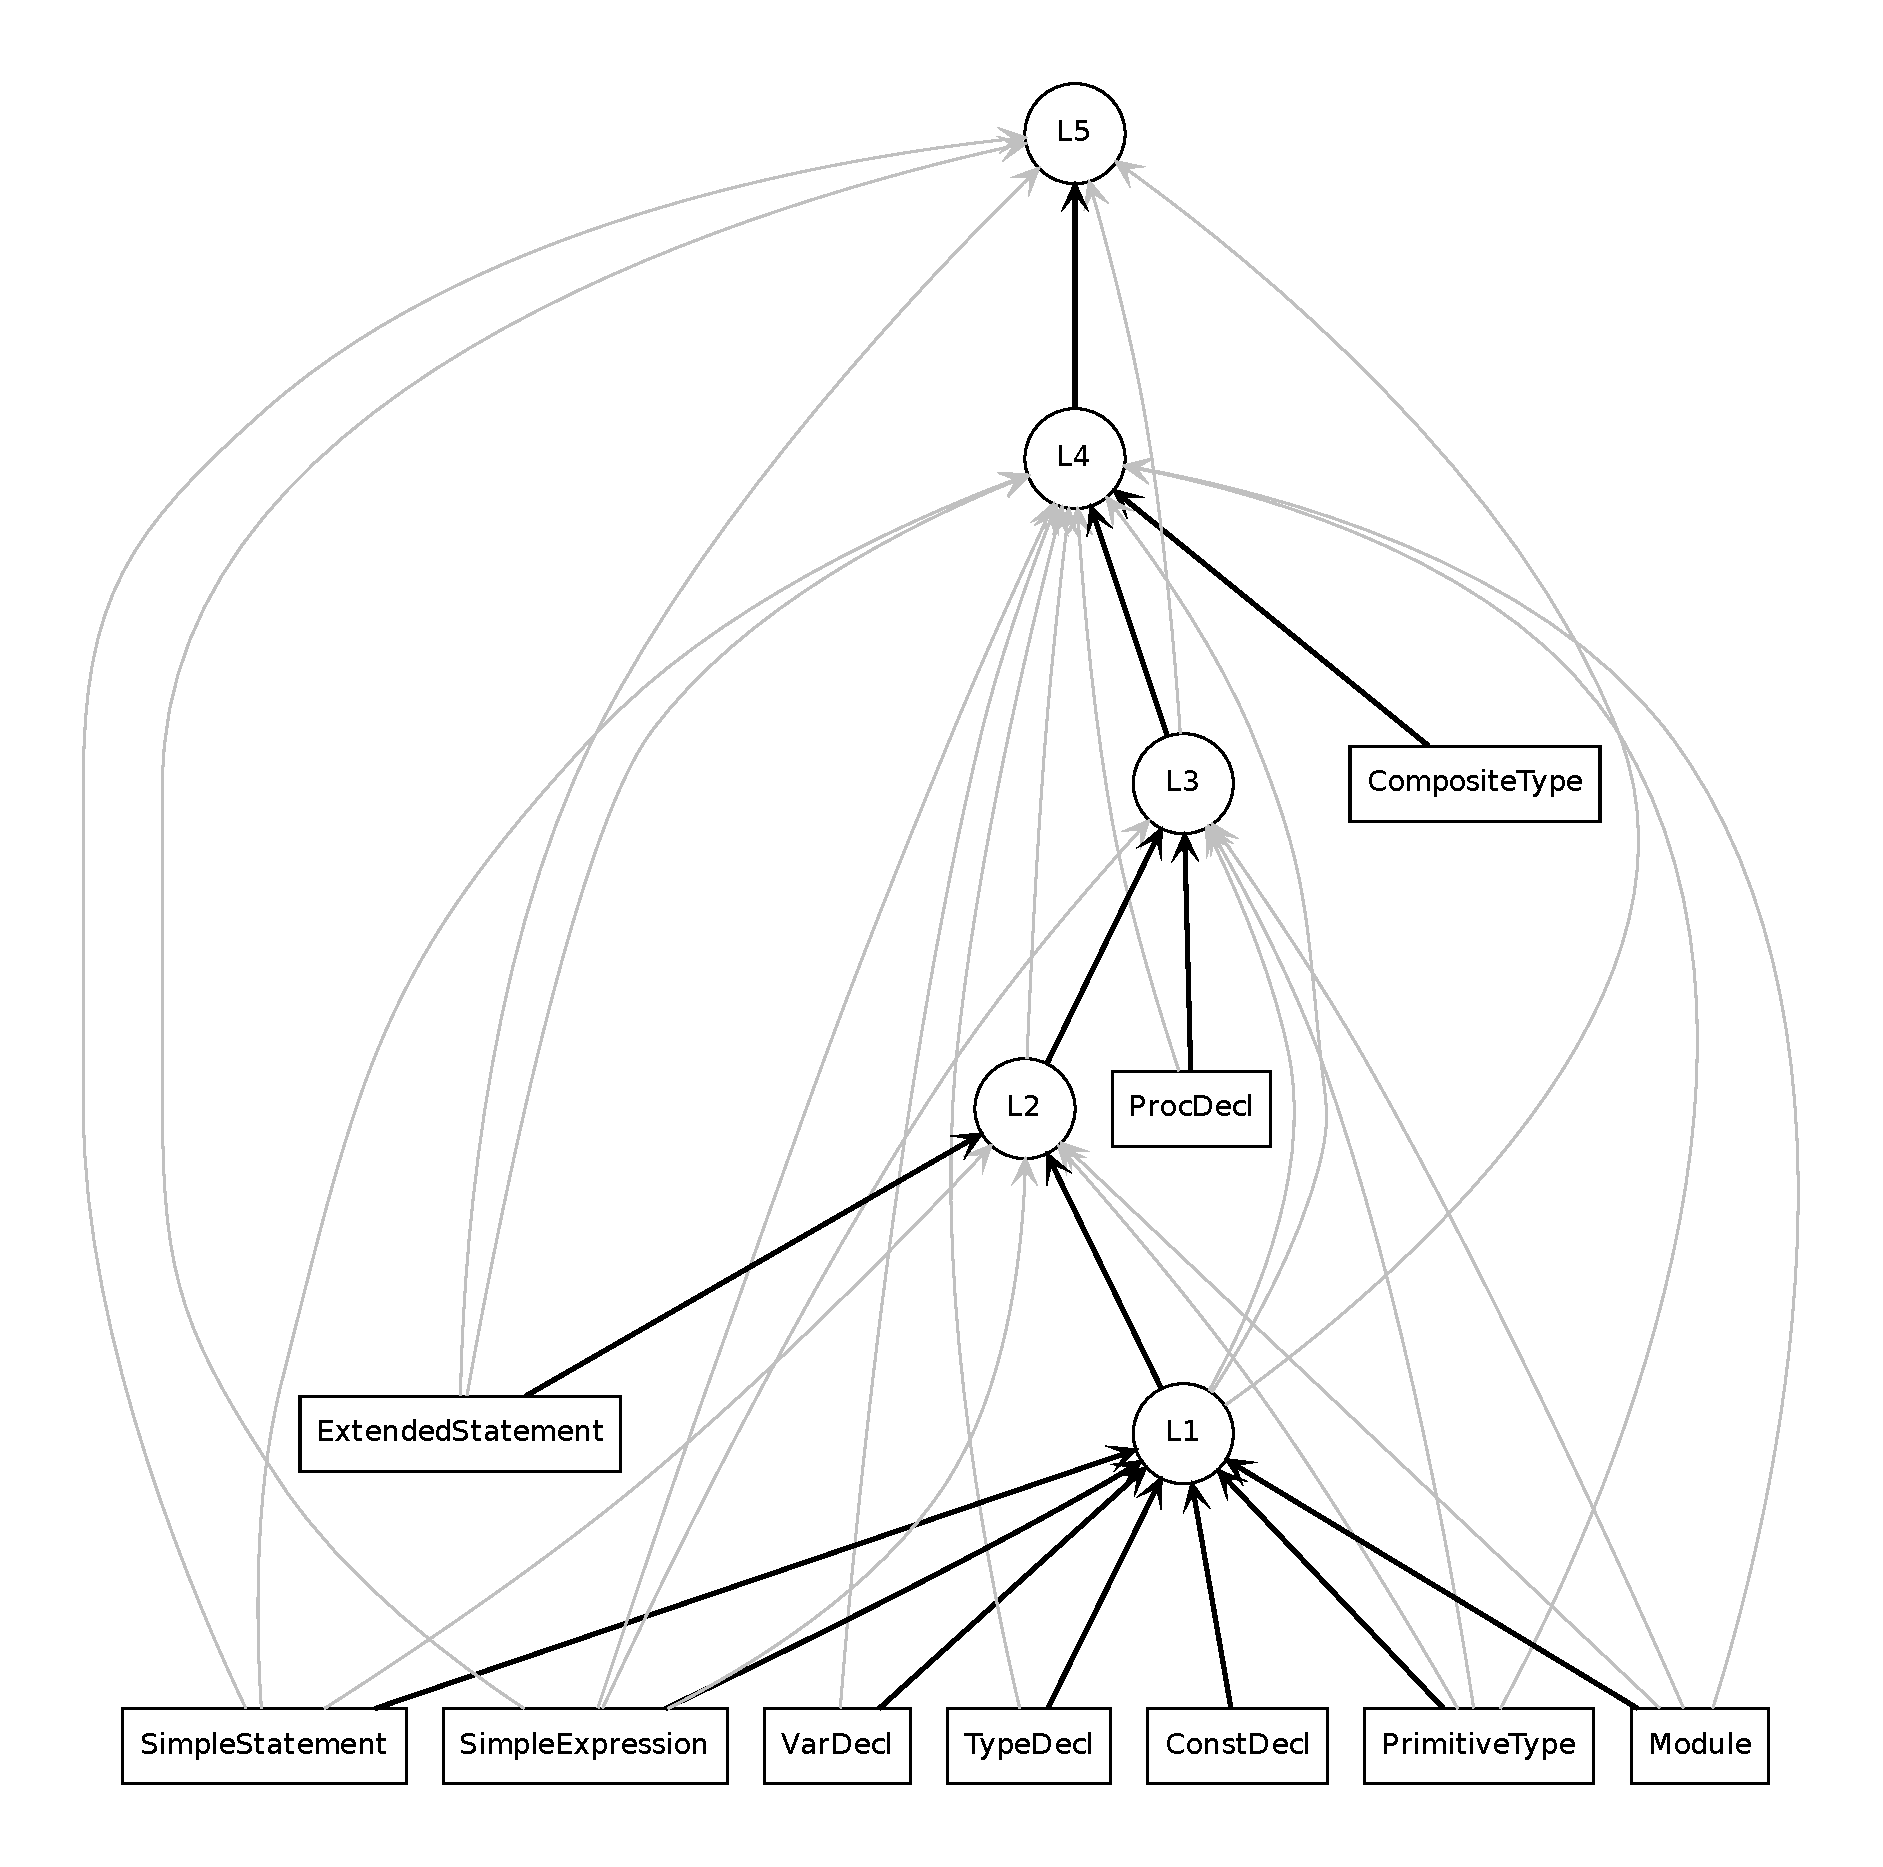
\includegraphics[height=13cm, width=14cm]{ocaml/depend.pdf}
\end{center}
\label{ocamlmoddep}
\caption{OCaml Implementation Module Dependencies}
\end{figure}

\subsection{Type-driven Transformers}

In this section we describe type-driven transformers of a certain kind which are 
massively used in OCaml implementation. Namely, all the tasks excluding parsing
are expressed using solely the transformers of this kind. ``Type-driven'' means that
the semantics of transformers is completely determined by the transforming type; 
so all transformers can be constructed mechanically from the type definitions.
The converse is also true --- the type-driven transformer unambigiously defines
some type. We heavily utilize this property --- actually there is not a single 
type definition in the implementation: all types are introduced implicitly 
and inferred from the transformation functions. Another property of transformers
is their extensibility: each transformer operates on a data of a partially-defined, 
or \emph{open}, type. Thus transformers for some types can be combined by a certain primitive
to provide a transformer for the union type which still remains open and so can be
combined later on. As a result we can construct a highly modular structure of
transformers each of which implements some task on a certain trait of some general
data structure. 

To implement this kind of approach a certain support from a host language type 
system is needed. OCaml provides such a support in particular by mean of 
\emph{polymorphic variant} types~\cite{PV}. In short, polymorphic variant types allow to 
share the same constructor between the different variant types with possibly different 
types and numbers of arguments. Polymorphic variant type need not (but can) be explicitly
declared. Another feature of polymorphic variant types is that they can be open --- in each
context only some of their constructors may be known. Polymorphic variants in OCaml 
can be used to express the solution for the \emph{expression problem}~\cite{Exproblem, PVReuse} --- 
that is, the problem of modular and type-safe implementation of extending data structure 
processing. 

We illustrate the construct of type-driven extensible transformers by the canonical
example --- expression evaluator. The idea is to implement evaluator as a
collection of functions each of which evaluates only the limited subset of expression's
nodes and then to combine them to construct the evaluator of the whole expression.

First, consider the function which transforms only two expression nodes ---
addition and subtraction\footnote{Polymorphic variant type constructors are lexically distinguished
from the regular ones by the backquote as their first character.}:

\begin{lstlisting}[language=ocaml]
let rec evalAddSub ext expr =
  let self = evalAddSub ext in
  match expr with
  | `Add (x, y) -> self x + self y
  | `Sub (x, y) -> self x - self y
  | z -> ext self z
\end{lstlisting}

Here \lstinline{ext} stands for the extension function --- that is, the function which
transforms the rest of polymorphic variant type's constructors besides those transformed 
by \lstinline{evalAddSub}. Note that since we want to transform potentially recursive 
structures we have to provide extension function with it's own extension function which 
should be able to transform the all nodes of expression, including \lstinline{`Add} and
\lstinline{`Sub}. This extension function (``\lstinline{self}'') is acquired by partial
application \lstinline{evalAddSub} to \lstinline{ext}.

Now we can provide two additional functions for evaluating identifiers in some state 
\lstinline{s} and multiplication:

\begin{lstlisting}[language=ocaml]
let rec evalIdent s ext expr =
  let self = evalIdent s ext in
  match expr with
  | `Ident n -> s n
  | z -> ext self z
\end{lstlisting}

\begin{lstlisting}[language=ocaml]
let rec evalMult ext expr =
  let self = evalMult ext in
  match expr with
  | `Mul (x, y) -> self x * self y
  | z -> ext self z
\end{lstlisting}

Note that the semantics of these functions is almost completely type-driven; despite
we do not have any type declaration here we actually think in terms of types, not
in terms of implementation details. The only concrete implementation-dependent feature
is the essense of constructor-specific transformation; we'll get rid of this specificity 
later. Note also that these functions are completely independent of each other; thus, they 
can be implemented in a different compilation units or provided at arbitrary moments of 
program execution.

Now we introduce the combinator which plays role of type sum:

\begin{lstlisting}[language=ocaml]
let (++) left right = fun ext s -> 
  left (fun self -> right (fun _ -> ext self)) s
\end{lstlisting}

This combinator takes extensible transformers for some open types and provides extensible transformer 
for the type of their sum. This is trivially achieved by providing appropriate extensions for each ``summands''.
For example,

\begin{lstlisting}[language=ocaml]
let evalAddSubIdent s = evalIdent s ++ evalAddSub
\end{lstlisting}

is (an extensible) function which evaluates expressions with nodes \lstinline{`Add}, \lstinline{`Sub} and
\lstinline{`Ident}. This function can further be combined:

\begin{lstlisting}[language=ocaml]
let evalAddSubIdentMult s = evalAddSubIndent s ++ evalMult
\end{lstlisting}

et cetera. 

When we need to actually apply these transformers to a data structure we have to provide
some sort of ``ultimate'' extension function; it is easy to see that this function is just
an application; in the following snippet

\begin{lstlisting}[language=ocaml]
let apply f x = f x

let x = 
  evalAddSubIdent 
     (function "a" -> 1 | "b" -> 2 | "c" -> 3 | "d" -> 4)
     apply 
     (`Add (
        `Sub (`Ident "a", 
              `Mul (`Ident "b", `Ident "c")
        ), 
        `Ident "d"
      )
     )
\end{lstlisting}

the name \lstinline{x} would be bound to \lstinline{-1}.

In the previous examples we considered some concrete transformers --- evaluators.
However a simple generalization would let us abstract this specificity away. Namely, 
we preserve the overall control flow of the transformers but parameterize the
actions carried out for each constructor. The generalized version of the first 
transformer is presented below:

\begin{lstlisting}[language=ocaml]
let rec gmapAddSub t ext expr =
  let self = gmapAddSub t ext in
  match expr with
  | `Add (x, y) -> t#add expr (self x) (self y)
  | `Sub (x, y) -> t#sub expr (self x) (self y)
  | z -> ext self z
\end{lstlisting}

Here \lstinline{t} stands for the constructor-wise transformer encoded
as an \emph{object} with methods ``\lstinline{add}'' and ``\lstinline{sub}''.
Each method takes the results of the same transformation applied to the
direct counterparts of matched value and that value itself as arguments
and returns the result of the transformation. Now the evaluation function
can be expressed as

\begin{lstlisting}[language=ocaml]
let evalAddSub ext expr = 
  gmapAddSub (object
                method add _ x y = x + y
                method sub _ x y = x - y
              end) ext expr
\end{lstlisting}

The type system of OCaml allows objects to be implicitly typed: there is 
no need to declare object types ``in advance''. Another feature of object
types is that they can be polymorphic. This means that the definition of
\lstinline{gmapAddSub} does not introduce any artificial type restrictions
on a set of encoded transformations. For example, the copy transformation
can be expressed using the same function but different object (of different but
``compatible'' type):

\begin{lstlisting}[language=ocaml]
let copyAddSub ext expr =
  gmapAddSub (object
               method add _ x y = `Add (x, y)
               method sub _ x y = `Sub (x, y)
             end) ext expr
\end{lstlisting}

Since each concrete transformation can be expressed as a partial application of
some generic \lstinline{gmap...} function to an object-encoded per-constructor
transformation the implementation of the typ-sum combinator can be left completely 
unchanged. For example, the expression evaluator for partially defined expression
of addition, subtraction and identifiers can be implemented as

\begin{lstlisting}[language=ocaml]
let evalAddSubIdent s = 
  gmapAddSub (object
                method add _ x y = x + y
                method sub _ x y = x - y
              end) ++
  gmapIdent (object method ident _ n = s n end)
\end{lstlisting}

In this approach we can easily construct transformations via combining and
extending the predefined set of object-encoded per-type transformers; in 
particular the following transformer generator was extensively used in the course
of the implementation (as always we show the version for \lstinline{`Add}-\lstinline{`Sub}
type):

\begin{lstlisting}
let mapT f = object
               method add e x y = f e (`Add (x, y))
               method sub e x y = f e (`Sub (x, y))
             end
\end{lstlisting}

The final generalization consists of ``lifting'' the transformation functions
over some monad~\cite{Monads}. The implementation is straightforward so we omit it
here; we note that the parameterization over a monad is implemented using OCaml functors. 
In this implementation of Oberon0 we used three monads --- a variant 
of exception monad called \lstinline{Checked}, identity monad \lstinline{Id} and list 
monad \lstinline{List}. We refer to the monad-specific transformation functions for 
the two former monads as \lstinline{cmap} and \lstinline{imap} respectively.

\subsection{Scanning, parsing and pretty-printing}

For scanning, parsing and pretty-printing we use the parser- and printer-combinator
library called Ostap\footnote{http://caml.inria.fr/cgi-bin/hump.en.cgi?contrib=513}. 

Ostap comprises of the set of regular monadic parser-combinators~\cite{MonadicParserCombinators} 
and a syntax extension for OCaml which allows to bind syntax definitions in
EBNF directly into compiler sources thus avoiding parser generation phase. The syntax
extension in turn is implemented using Camlp4/Camlp5 syntax extension 
tool. 

As example consider the parser definition for simple statements of L1:

\begin{lstlisting}[language=ocaml]
ostap (
  parse[ref][expr][stmt]: 
    assignment[ref][expr] 
  | ifStatement[expr][stmt] 
  | whileStatement[expr][stmt];
  assignment[ref][expr]: dst:ref ":=" src:expr {`Assign (dst, src)};
  ifStatement[expr][stmt]: 
    key["IF"] cond:expr 
       key["THEN"] thenPart:oseq[stmt]
       branches:(-key["ELSIF"] expr -key["THEN"] oseq[stmt])*
       elsePart:(-key["ELSE"] oseq[stmt])?
    key["END"] {
    `If ((cond, thenPart)::branches, listify elsePart)
  };
  whileStatement[expr][stmt]: 
    key["WHILE"] cond:expr key["DO"] stmts:oseq[stmt] key["END"] {
    `While (cond, stmts)
  }
)
\end{lstlisting}

The parser is implemented in a high-order form --- it takes as arguments a parsers
for references, expressions and statements as well. The structure of rules
repeats that of regular EBNF. We use here some predefined combinators --- \lstinline{key} 
and \lstinline{oseq} --- which are defined in a separate module. \lstinline{key} recognizes
its string argument making sure that the next symbol is a word delimiter while \lstinline{oseq}
parses a possibly empty semicolon-delimited items specified by its argument. Note that 
parameterization by statement parser \lstinline{stmt} makes the whole parser \emph{open} ---
it parses wider language than merely assing-if-while with assign-if-whiles as substatements.

The definition of parser becomes closed at the client level; for example, L1-statements
parsed with the following parser:

\begin{lstlisting}[language=ocaml]
statement: !(SimpleStatement.parse)[reference][expression][statement];
\end{lstlisting}

Here \lstinline{!(...)} used to bind arbitrary OCaml expression into EBNF rule (we use it
to call parser \lstinline{parse} from module \lstinline{SimpleStatement}), \lstinline{reference} and
\lstinline{expression} designate the parsers for L1 references and expressions respectively.

Similarly, we can easily combine different parameterized parsers to obtain parsers for more
complex constructs. For example, extended statements of L2 are parsed with the following
definition:

\begin{lstlisting}[language=ocaml]
statement[ref][cexpr][expr][stmt]: 
  !(SimpleStatement.parse)[ref][expr][stmt]
| !(ExtendedStatement.parse)[ref][cexpr][expr][stmt];
stmt: statement[reference][expression][expression][stmt];
\end{lstlisting}

Here we combine parser for simple statements with parser for extended statements (``CASE'' and ``FOR'')
into the one. Note the lack of semantic actions --- there are completely defined in corresponding
parsers. Note also that the types of syntax trees, provided by these two combined parsers are completely 
independent on each other. At the top level these types are combined by the compiler; this implementation 
is completely type-safe.

Besides parser-combinators Ostap contains a set of pretty-printer combinators, which are
in fact merely wrappers for the standard pretty-printing module \lstinline{Format}. To
convert the original AST into printing functions using these combinators we again
use type-driven transformers; for example, the expression pretty-printer looks like
the following:

\begin{lstlisting}[language=ocaml]
let gprint ps ext expr =
  let b x = hovboxed (listBySpaceBreak x) in
  let op (s, p) = string s, p in
  let w p' (x, p) = if p' < p then rboxed x else x in 
  imap  
    (object 
       method binop _ o x y = 
         let s, p = op (ps#binop o) in b [w p x; s; w p y], p
       method unop  _ o x   = 
         let s, p = op (ps#unop o) in b [s; w p x], p
       method const _   x   = ps#const x
     end
    )
    ext
    expr
\end{lstlisting}

Note that apart from extensibility this pretty-printer is generalized in yet another 
dimension --- namely, it is abstracted away from the concrete syntax. The \emph{ps}
parameter designates \emph{printing scheme} which encapsulates the concrete
syntax of arithmetic operators as well as their priorities. This allows to handle
both pretty-printing and C generation.

\subsection{Name analysis}

The name analysis in OCaml implementation in fact performs the following tasks:

\begin{itemize}
\item \emph{Kind analysis} --- the verification of proper usage of each name for each context this
name appears in. For example, the left side of an assignment should designate a variable or procedure argument,
all references in a constant expression should designate constants etc.
\item \emph{Constant evaluation} --- the replacement of each constant expression by
its value;
\item \emph{Proper name analysis} --- establishing the relation between the usage of
named entity and its declaration;
\item \emph{Name disambiguation} --- assigning to each named entity in the program a unique
name preserving its declaration-usages coherence.
\end{itemize}

From the technical point of view the functionality of name analysis is again implemented as a 
one-pass monadic transformer with the exception monad \lstinline{Checked} and a mutable symbol 
table. This transformer actually propagates the results of reference analysis through the 
entire AST. For example, for extended statements of L2 the transformer itself looks like
the following:

\begin{lstlisting}[language=ocaml]
let resolve ref cexpr expr ext stmt =
  cmap ext 
       (mapT (fun _ s -> Monad.Checked.return s)) 
       ref 
       cexpr 
       expr 
       stmt
\end{lstlisting}

Note that we encode various contexts parametrically: here ``\lstinline{ref}'' corresponds
to the reference checking function, ``\lstinline{cexpr}'' --- to the constant expression 
checking function, ``\lstinline{expr}'' --- to the gerenic expression checking function
so actually we perform kind analysis by discriminating the cases already encoded in
the AST data structure in a type-parametric manner. 

Each expression checking function is itself aquired by applying the type-driven transformer 
for expressions to a reference-checking routine of a certain kind. For example, the expression 
name analysis for L1 is encoded in the following manner:

\begin{lstlisting}[language=ocaml]
let reference env ext = 
  function
  | `Ident name -> 
       env#lookup name >= 
       (function x -> `Ident (env#extractInternal x, x))
  | x -> ext x

let expression env expr = 
  SimpleExpression.resolve (reference env) expr 
\end{lstlisting}

Here ``\lstinline{ext}'' is an extension for name-analysis function for references. This 
extension is provided later in the extended languges to handle the references of other kinds.

Name analysis converts the initially parsed AST into the structure of incompatible 
type. From one hand this approach enforces the safety of the compiler since, for example, an attempt
to typecheck an unresolved program will not pass the typechecker; on the other hand this
safety has its cost --- for example, a separate pretty-printer is required for a
name-resolved tree. 

\subsection{Type checking}

The type checking in OCaml implementation follows the common scheme: we map the name-resolved
AST of the program into its type-annotated counterpart. This transformation is
actually superfluous for Oberon-0 since we do not need type information neither for
source-to-source transformation nor for the C generation; yet we still implemented it in
a generic form just to demonstrate the approach.

The most work in the type-checking phase is done at the expression level. Since the 
initial AST does not have any type information (and even does not have any ``placeholders'' 
for it) we map each expression into an isomorphic structure by \emph{pairing} each node 
with the corresponding type. Note that this transformation does not preserve the type of
the expression tree; it can not even be expressed by some parameterization of the
expression tree type. For simplicity consider the expressions made of binary operations,
constants and identifiers; then the type-pairing transformation would have the type

\begin{lstlisting}[language=ocaml]
([< `Binop of 'a * 'a | `Const of 'b | `Ident of 'c ] as 'a) ->
([> `Binop of 'd * 'd | `Const of 'b | `Ident of 'c ] * typ as 'd)
\end{lstlisting}

where \lstinline{typ} stands for the type-representing type; in the actual implementation
we should also take care of the extensibility of the type-checkers. All type-pairing
transformations are performed using type-driven transformers.

Besides annotating the expression trees with the type information the type-checking 
phase also performs the checking itself; due to the simplicity of the type system
this checking consists of merely comparisons between expected and actual types of expressions
in a various syntactic contexts.

\subsection{Source-to-source transformation}

All source-to-source transformations are actually performed on the name-resolved AST; then
the modified AST is pretty-printed. These transformations maintain all the invariants of
the name-resolved AST so it subsequently can be typechecked or undergo further 
transformations. Note that this approach simplifies the implementation a lot since all name 
disambiguation is performed on the name resolution stage.

Since sometimes we need new names to be generated (for example for capturing the upper bounds of
FOR statements during lowering) we also provide the name generation helper which is constructed
on the name resolution stage and then is passed to the transformation functions as a parameter.

In the following subsections we consider the individual transformations.

\subsubsection{Lowering}

Lowering projects extended statements of L2 (FOR- and CASE- statements) into the composition
of simple statements of L1. This transformation is implemented using monadic transformation
using list monad since generally we transform a single statement (say, FOR) into the list
of statements. The skeleton code for the transformation is as follows:

\begin{lstlisting}[language=ocaml]
let lower ext stmt =
  let module M = SimpleStatement.Mapper (Monad.List) in 
  let module E = ExtendedStatement.Mapper (Monad.List) in
  M.gmap 
    (fun self stmt ->
       E.gmap (ext self)
              (object
                 method case _ e b s = ...
                 method forc _ i l u s b = ...
               end
              ) 
              Monad.List.return 
              Monad.List.return 
              Monad.List.return 
              stmt
    )
    (SimpleStatement.mapT (fun _ s -> [s])) 
    Monad.List.return 
    Monad.List.return
    stmt
\end{lstlisting}

Here ``\lstinline{ext}'', as usually, stands for the extension transformation. This skeleton
code just propagates the lowering transformation through all the constructs of the AST. All
nontrivial work is done by methods ``\lstinline{case}'' and 
``\lstinline{forc}''\footnote{``\lstinline{for}'' is a reserved word in OCaml.} which are 
called when the corresponding construct is encountered in the tree.

Method ``\lstinline{case}'' takes the original AST node for the CASE statement 
(which actually is never used for the lowering, hence the wildcard symbol ``\lstinline{_}'' 
as a parameter placeholder), and its immediate subtrees --- key expression ``\lstinline{e}'',
list of conditional branches ``\lstinline{b}'' and the else branch ``\lstinline{s}'' --- and transforms it 
into the compound \mbox{IF-THEN-ELSIF-...-END} statement with the key value captured into the fresh variable.
Method ``\lstinline{forc}'' operates in a similar manner.

During lowering we sometimes need to construct new fragments of AST; we facilitate this task
with the help of \emph{quotations}. A quotation is just a parser which converts a parameterized 
string into a fragment of AST. For our needs the following definition of quotation parsers turned out 
to be sufficient:

\begin{lstlisting}[language=ocaml]
let ostap (
  qexpr[qc]: "$" i:ident {qc i};
  expr [qc]: !(SimpleExpression.parse)[qexpr qc];
  stmt [qc]: !(SimpleStatement.parse)[expr qc][expr qc][stmt qc];
  stmts[qc]: oseq[stmt qc] -EOF
)
\end{lstlisting}

In short, our quotations parse arbitrary simple expressions and statements with the special form of
references --- identifiers preceded by the symbol ``\$''. Each identifier is substituted with a
some subtree during the parsing process. The substitution function ``\lstinline{qc}'' --- 
\emph{quotation context} --- is provided as a parameter for the parser. 

With the help of quotations the transformation implementation becomes more concise --- for example, 
we can use the expression

\begin{lstlisting}[language=ocaml]
   qe ["k", k; "l", l; "u", u] "($k >= $l) & ($k <= $u)"
\end{lstlisting}

for checking if the value of CASE key expression ``\lstinline{k}'' fits in the range with boundaries
``\lstinline{l}'' and ``\lstinline{u}'' of a certain case branch instead of tedious encoding of corresponding 
AST with its node constructors. Here ``\lstinline{qe}'' is just a wrapper for the parser ``\lstinline{expr}''
defined in the former code snippet which additionally takes a quotation context represented by an associative 
list.

Note that the quotation functionality is implemented in a completely independent manner of the ``main'' parsers ---
none of them are aware of quotation definitions which are kept completely local to the lowering function. Note also
that quotation parsing provides already a name-resolved AST since all quotation arguments are substituted with 
the name-resolved subtrees.

\subsubsection{Type lifting}

Type lifting moves type definitions enclosed in procedures to the top level. These definitions can not be
kept inside the procedures since after procedure lifting some references to them might run out
of scope. This transformation is handcoded; nothing interesting is done here since all type names are 
already disambiguated.

\subsubsection{Procedure lifting}

Procedure lifting in OCaml implementation comprises two transformations:

\begin{itemize}
\item \emph{Elementary procedure lifting} which moves nested procedures to the top level. This transformation, 
preceded by the type lifting, is performed prior to C generation for the language L4. Similarly to the type 
lifting, this is just a primitive transformation which is handcoded.

\item \emph{Lambda-lifting} which promotes (some) local variables and parameters of a procedure into the
argument lists of its nested subprocedures with corresponding call statements modifications. Note that in
our implementation lamba lifting \emph{does not move} procedure declarations to the top level.
\end{itemize}

While elementary lifting is used to project L4 into itself prior to C generation the lambda lifting
projects L5 into the some language which is actually a superset of L4 (since even after the lambda-lifting 
the program can still violate some L4 visibility rules for procedure declarations). 

The lambda-lifting implementation is decomposed into the following passes:

\begin{itemize}
\item \emph{Inspection}. During this stage we traverse the AST of the program and for each procedure collect the 
names of all called procedures and all used non-local variables. The most of the 
traversal is performed using type-driven transformers with identity monad; the gathered information is 
collected in a mutable data structure. 

\item \emph{Propagation}. On this stage we propagate the collected non-local usage information through the call
graph represented by the mapping between the caller and callees. This pass is handcoded.

\item \emph{Modification}. During this stage the program is rewritten into the lambda-lifted form using the information
provided by the previous two stages. This rewriting involves changing the declaration of procedures and
their call sites, replacing usages of non-local variables into usages of procedure arguments, passed by 
reference, and introducing the type synonyms for the types of those local variables whose usages in 
nested procedures resulted in passing them as parameters. Most of the work is again performed by
type-driven transformers with identity monad.
\end{itemize}

Note that we again heavily utilize the name disambiguation performed on the name resolution stage --- we do
not need neither new names for the lifted procedure arguments nor the correspondence between newly introduced
formal and actual parameters since we can simply use the same name for the formal and actual parameter.

Despite the fact that the application of type-driven monadic transformers simplified the implementation a lot the
lambda-lifting is still the most cumbersome and hard-to-understand part of the compiler.

As an observable result consider the following L5 program:

\begin{lstlisting}[language=oberon0]
MODULE L;
  PROCEDURE T;
    VAR i : INTEGER; a : ARRAY 10 OF INTEGER;
    PROCEDURE Init;
    BEGIN
      FOR i:=1 TO 10 DO a[i] := i END
    END Init;
  BEGIN
    Init ()  
  END T;
BEGIN
  T ()
END L.
\end{lstlisting}

The source-to-source transformation is performed in the following order:

\begin{itemize}
\item Type lifting;
\item Lambda-lifting;
\item Procedure lifting;
\item Lowering.
\end{itemize}

As a result the following L4-code in produced:

\begin{lstlisting}[language=oberon0]
MODULE L;
  TYPE
    typename = ARRAY 10 OF INTEGER;
  PROCEDURE globaltopTInit 
  (VAR globaltopTa : typename; 
   VAR globaltopTi : INTEGER);
  VAR
    upb : INTEGER;
  BEGIN
    globaltopTi := 1; 
    upb := 10; 
    WHILE (1 > 0) & (globaltopTi <= upb) OR 
          (1 <= 0) & (globaltopTi >= upb)
      DO
        globaltopTa[globaltopTi] := globaltopTi; 
        globaltopTi := globaltopTi + 1
      END
  END globaltopTInit;
  PROCEDURE globaltopT ();
  VAR
    globaltopTi : INTEGER;
    globaltopTa : typename;
  BEGIN
    globaltopTInit (globaltopTa, globaltopTi)
  END globaltopT;
  BEGIN
    globaltopT ()
END L.
\end{lstlisting}

\subsection{Code generation}

There is no dedicated code generation pass in OCaml implementation --- we consider C representation
as an alternative concrete syntax for the name-resolved (and lifted) AST. Pretty-printers for the relevant
structures (simple expressions with L4 references, simple statements with procedure calls, 
type-, variable- and procedure declarations) are implemented in a generic form: they take a
printing scheme which encapsulates the concrete syntax elements as an additional
parameter. Note that we need a name-resolved tree to distinguish, for example, referenced-passed
function parameters from value-passed ones in both function argument declaration list, all
their usages within the function body and actual parameters of function invocation.

\subsection{Artifacts}

\subsection{Observations}

\subsection{Conclusions}

\section{Kiama}

Kiama is a collection of domain-specific languages (DSLs) each addressing a typical language processing task~\cite{Sloane11}.
The DSLs are embedded in the Scala general-purpose programming language~\cite{Odersky10d}.
All of the DSL code is standard Scala and is just compiled by the normal Scala compiler.
This approach means that a Kiama-based program can use the DSLs where appropriate, but it can fall back on Scala where more general computation is required.
The result is a very lightweight approach to language processing since each DSL is simple and has a small implementation.

We distinguish between the following kinds of components, each supported by a particular DSL or coding approach.

\begin{itemize}

\item \emph{Parsers} that read program text and build \emph{abstract syntax trees (ASTs)}.
We use combinators from the standard Scala library to write parsers~\cite[chapter 33]{Odersky10d}.

\item \emph{Analysers} that decorate ASTs with information and check the conformance of that information to language rules.
The decorations take the form of \emph{attributes} associated with tree nodes.
Kiama's \emph{attribute grammar DSL} provides a notation for expressing attribute computations~\cite{Sloane12}.

\item \emph{Transformers} that restructure ASTs while staying within a single syntax.
We write transformers using Kiama's \emph{strategic term rewriting DSL} which is based on the Stratego language~\cite{Visser04,Visser07a}.

\item \emph{Translators} that convert an AST conforming to one syntax into an AST conforming to another syntax.
We write translators using normal mutually-recursive Scala functions.

\item \emph{Pretty printers} that convert ASTs into text.
We write rules that govern pretty printing using a Kiama version of a well-known \emph{pretty-printing DSL}~\cite{Swierstra08a}.

\end{itemize}

\noindent
Typically, each component is a separate Scala trait.
We use the mixin facilities of Scala to assemble components into language implementations~\cite[chapter 12]{Odersky10d}.
Thus, Kiama-based programs are extremely modular but this modularity does not impact the language processing DSLs.

Sections~\ref{sec:kiama-scanparse} to \ref{sec:kiama-codegen} describe how the individual components of the Oberon-0 compiler were written.
Section~\ref{sec:kiama-artifacts} describes the overall structure of the Kiama Oberon-0 implementation, including how the components relate to each other and are combined to make the challenge artifacts.
Section~\ref{sec:kiama-observe} steps back from the detail to make some observations about the strengths and weaknesses of the Kiama approach.

% FIXME: need to mention that code fragments are somewhat simplified?  Eg no positioned in the parser

\subsection{Scanning and parsing}
\label{sec:kiama-scanparse}

The abstract syntax trees built by the parsers are defined using a standard object-oriented approach.
Each non-terminal of the grammar is an abstract class with concrete sub-classes for each variant of that non-terminal.
The concrete classes in the AST definition are defined using Scala case classes~\cite[chapter 15]{Odersky10d}.
Case classes are normal classes, but also share some properties with algebraic data types in functional languages.
For example, instances can be created without the \verb|new| keyword and their components can be extracted using pattern matching.
We will see examples when we discuss the AST processing phases in subsequent sections.
For now, here is the fragment of the AST definition that defines assignment statements and some forms of expression.

\begin{verbatim}
abstract class Statement extends SourceASTNode
case class Assignment (desig : Expression, exp : Expression)
  extends Statement

abstract class Expression extends SourceASTNode
case class IntExp (v : Int) extends Expression
case class AddExp (left : Expression, right : Expression)
  extends Expression
\end{verbatim}

The versions of the Oberon-0 compiler that output C code first construct an AST to represent that code.
We use the term \emph{source AST} to refer to the AST of the Oberon-0 source program and \emph{target AST} to refer to the AST of the C target program.
The principles for defining the target AST are the same as for the source AST.
Target ASTs are produced by translators instead of by parsers (see Section~\ref{sec:kiama-codegen}).

Parsers are written using Scala packrat parsing library combinators~\cite[chapter 33]{Odersky10d}.
Complex parsers can be constructed from basic ones in a style that mimics context-free grammar productions.
The correspondence is very close, including the ability to use left-recursion~\cite{Warth08}.
The parser for an assignment statement shows a typical use of the main combinators.

\begin{verbatim}
val assignment = (lhs ~ (":=" ~> expression)) ^^ Assignment
\end{verbatim}

\noindent
where \verb|lhs| and \verb|expression| are parsers defined elsewhere.
A literal string is converted implicitly into a parser that just accepts that string.
The \verb|~| operator sequences two parsers to make a parser that returns a pair of the values of its operands.
The \verb|~>| operator also sequences, but throws away the value of its left operand.
The \verb|^^| operator transforms the result of a parser using an arbitrary function.
In the example the \verb|Assignment| constructor is used to build an AST node.

There is no separate scanning phase.
Parsers for lexical symbols are constructed directly from regular expressions.
For example, an identifier is parsed by first rejecting keywords and then accepting suitable strings of characters.

\begin{verbatim}
val ident = not (keyword) ~> "[a-zA-Z][a-zA-Z0-9]*".r
\end{verbatim}

\noindent
(The \verb|r| method of a string converts it to a regular expression.)

White space is skipped by the library parsers for literals and regular expressions.
The Scala library supports the definition of white space using a regular expression.
Oberon-0 white space includes comments that can nest.
Rather than define an awkward non-standard regular expression for nested comments, we use a Kiama extension of the Scala library that allows white space to be defined by a parser.
Therefore, we can define Oberon-0 white space as follows, where \verb|whiteSpace| is the default white space regular expression and \verb|any| parses any character.

\begin{verbatim}
val whitespaceParser = rep1 (whiteSpace | comment)
val comment = "(*" ~ rep (not ("*)") ~ (comment | any)) ~ "*)"
\end{verbatim}

\subsection{Name analysis}

The analysis components implement a single method that is called once for each node in the source AST.
Analyses compute persistent attributes of AST nodes and can use attributes of previous analyses.
Attributes are computed lazily (i.e., on demand and their values are cached), so an analysis does not have to worry about the order in which attributes are computed.
Since attributes cache their own values independently of the AST, the AST is unchanged by an analysis.

An analysis can produce messages to be reported to the user.
Messages are reported using a simple Kiama utility library that collects them with their code positions.
The compiler driver prints the messages when all analyses are done.
Phases such as code generation that rely on a correct source AST are skipped if any messages have been produced.

Name analysis checks and reports errors relating to the declaration and use of identifiers in the source program.
We compute an environment for each AST node that contains exactly those bindings that are visible to that node according to the scoping rules of Oberon-0.
The environment is threaded through the AST using a chain of attributes that is modelled after similar constructs in dedicated attribute grammar languages~\cite{Kastens94}.
An attribute chain encapsulates a pattern of attribution that reaches each node from its parent, visits each of its children recursively from left to right, then leaves the node to the parent.
At each point along the way the value of the chain can just be passed along or a new value can be computed, usually based on the value of the chain coming into that point.

Kiama provides support for defining chains where the default threading behaviour is provided but can be overridden by defining partial functions that match on AST nodes.
For example, the environment chain is defined to start at the root of the AST with an empty stack of scopes.
Some nodes define new scopes.
The value of the environment coming in to these nodes is the scope stack from the parent with a new empty scope pushed onto it.
The value that leaves such a sub-tree is the value used in the sub-tree with the top scope popped.
(It is important to remember that each of these values is a separate attribute, so no values are being updated.)
Similarly, a new binding is added to the environment chain at each declaration node.

The environment chain is accessed at each node representing an identifier use to match that use to a binding if possible.
The definition of the \verb|entity| attribute performs this operation and is typical of attribute definition by cases.

\begin{verbatim}
val entity : Identifier => Entity =
  attr {
    case n @ IdnDef (i) =>
      if (isDefinedInScope (n->(env.in), i))
        MultipleEntity
      else
        entityFromDecl (n, i)
    case n @ IdnUse (i) =>
      lookup (n->(env.in), i, UnknownEntity)
  }
\end{verbatim}

\noindent
The Kiama \verb|attr| function takes a single argument that is a partial function and wraps it with the lazy evaluation properties of attributes.
Attributes can be accessed in a functional style, or as used here, with the \verb|->| operator.
Thus, the \verb|env.in| is an attribute that is the value of the environment chain as it enters a node.
The expression \verb|n->(env.in)| obtains the value of that attribute at node \verb|n|.

It is common to define attributes by cases that pattern match on the AST node.
The \verb|entity| attribute is defined by two cases: one for defining occurrences of identifiers (\verb|IdnDef| nodes) and one for uses (\verb|IdnUse| nodes).
We might have that the identifier is already defined in the environment; in that case we return the special \verb|MultipleEntity|.
Otherwise, the definition is represented by a new entity that is computed from the declaration.
For example, a constant declaration will construct a new \verb|Constant| entity.
The entities can contain properties themselves or fields that refer to AST nodes from which properties can be derived.
A constant entity holds a reference to the constant declaration node from which the expression defining the constant can be obtained.
A similar scheme is used for other kinds of declaration.
An identifier use is associated with the entity for the corresponding declaration.
Thus, the second case of the example looks the identifier up in the environment, returning the entity found there if there is one, or returning the special \verb|UnknownEntity| if the identifier is not found.

Most checks are simple conditions on attributes.
For example, name analysis for the L1 language checks that no declaration is multiply-defined and that each use has an associated declaration.
These conditions are implemented by the following cases in the \verb|check| method. 
\verb|n| is the node that is being checked.

\begin{verbatim}
n match {
  case d @ IdnDef (i) if d->entity == MultipleEntity =>
    message (d, i + " is already declared")
  case u @ IdnUse (i) if u->entity == UnknownEntity =>
    message (u, i + " is not declared")
  ...
}
\end{verbatim}

\noindent
The \verb|message| method reports a message at the position of the AST node passed as its first argument.

This name analysis scheme extends easily to other language levels.
If no new declaration or scoping constructs are added, no changes need to be made.
The environment chain will simply traverse into the new constructs and the existing checks will be performed.
New declarations and scoping constructs can be accommodated by extending the definitions of the \verb|entityFromDecl| method and the environment chain.
For example, in the L3 name analyser the chain is adjusted to take into account procedure scopes.
New entities are added to represent procedures and parameters.
All environment processing, entities and checks from earlier levels are reused by the L3 analyser without change.

\subsection{Type checking}

The type analysis components of the Oberon-0 compiler are defined in a similar way to the name analysis components.
Each expression has a \verb|tipe| attribute\footnote{\texttt{type} is a reserved word in Scala.} that calculates its type from its contents, and an \verb|exptype| attribute that calculates the type as expected from the context.
The definitions of these attributes are straight-forward, so we omit them.
Identifier types are computed from their entities which give access to the declaration site containing declared or implied types.
Other expression types are given by their operators or literals.
Expected types are calculated by pattern matching on the parent of the expression.
For example, if the parent of an expression is an IF statement node, then the expected type of that expression is Boolean.

The L1 type analyser checks one simple condition: that the type of an expression is compatible with its expected type.
The exact definition of compatibility is provided by the \verb|isCompatible| method.
The definition of this method can be overridden in other language levels as the notion of compatibility changes.
The check itself can be left unchanged.

% FIXME: mention business of having an unknown and allowing it to appear anywhere?

\subsection{Source-to-source transformation}

Source-to-source transformation is used in the compiler to implement L2 FOR and CASE statements.
The analysis of these constructs is performed as described in the previous two section.
Between analysis and code generation, we \emph{desugar} these constructs into equivalent simpler constructs.
FOR statements are transformed into WHILE statements.
CASE statements are transformed into cascades of IF statements.

A transformation component implements a single method that takes as argument the root of a source AST and returns a possibly transformed AST.
As for analysis phases, a transformer at one level will call transformations at lower levels, so the transformations will be composed.
Transformations are implemented using Kiama's strategic term rewriting library.
For example, the L2 transformation is defined simply as

\begin{verbatim}
everywhere (desugarFor + desugarCase)
\end{verbatim}

\noindent
which tries to apply first the FOR transformation and, if that fails, the CASE transformation at every node in the tree.\footnote{An optimisation could be applied to attempt this transformation only in places where statements can occur.}

The actual FOR transformation is defined by the \verb|desugarFor| rule which simply pattern matches and returns the replacement tree fragment.
A FOR statement is translated into a block containing a declaration of a variable to hold the limit of the iteration and a WHILE statement to implement the loop.
This approach means that we do not need a different variable name for each FOR loop, since the scoping rules ensure that each loop will refer to the correct variable even if FOR loops are nested.
Note that the Oberon-0 source language does not allow nested blocks, but our abstract syntax does so that these kinds of transformations are easier to define.

\begin{verbatim}
val desugarFor =
  rule {
    case ForStatement (idnexp, lower, upper, optby, Block (Nil, stmts)) =>
      val limvarname = "limit"
      val limexp = IdnExp (IdnUse (limvarname))
      val incval = optby.map (_->value).getOrElse (1)
      val rincval = IntExp (incval)
      val cond = if (incval >= 0)
                     LeExp (idnexp, limexp)
                 else
                     GeExp (idnexp, limexp)
      Block (
        List (
          VarDecl (List (IdnDef (limvarname)),
                   NamedType (IdnUse ("INTEGER")))
        ),
        List (
          Assignment (clone (idnexp), lower),
          Assignment (clone (limexp), upper),
            WhileStatement (cond,
              Block (
                Nil,
                stmts :+
                  Assignment (clone (idnexp), AddExp (clone (idnexp), rincval))))
         )
      )
  }
\end{verbatim}

FIXME: too much code?

A complication in this rule is that we must be careful not to insert the same node in more than one place.
For example, when we want to refer to the \verb|limit| variable in the assignment statement, we must use a different node to the appearance of that variable in the condition.
Cloning is necessary because attributes are cached using the node identity as the key and the two nodes will in general have different attribute values.
In fact, the compiler is conservative when it comes to reuse of attribute values.
The attribute caches are cleared before any transformation to ensure that old, potentially incorrect values are not carried over to the new AST.

\subsection{Code generation}
\label{sec:kiama-codegen}

FIXME: translation components, lifting, pretty-printing

% PP: priority etc stuff for paren insertion

\subsection{Artifacts}
\label{sec:kiama-artifacts}

\begin{table}\centering
\begin{tabular}{|l|p{1.5cm}|p{1.5cm}|p{1.5cm}|p{1.5cm}|} \hline
& \multicolumn{4}{c|}{\emph{Language}} \\ \hline
& \emph{L1}    & \emph{L2}    & \emph{L3} & \emph{L4} \\ \hline
\emph{Parser}
& All          & All          & 2a, 3, 4  & 4         \\ \hline
\emph{Oberon-0 pretty printer}
& All          & All          & 2a, 3, 4  & 4         \\ \hline
\emph{Name analyser}
& All          & All          & 2a, 3, 4  & 4         \\ \hline
\emph{Type analyser}
& 2b, 3, 4     & 2b, 3, 4     & 3, 4      & 4         \\ \hline
\emph{Desugarer}
& 3, 4         & 3, 4         & 3, 4      &           \\ \hline
\emph{Lifter}
& 3, 4         & 3, 4         & 3, 4      &           \\ \hline
\emph{Oberon-0 to C Translator}
& 4            & 4            & 4         & 4         \\ \hline
\emph{C pretty printer}
& 4            & 4            & 4         & 4         \\ \hline
\end{tabular}
\caption{Kiama Oberon-0 components and their allocation to the artifacts.}    
\label{tab:kiama-artifacts}
\end{table}

The Kiama Oberon-0 challenge artifacts are constructed by combining components that each address a single phase for a particular language.
The components and their compositions into the artifacts are summarised in Figure \ref{tab:kiama-artifacts}.\footnote{
Actually, the implementation has two simpler language levels, Base and L0, below the first challenge level.
In our discussion, we have considered Base and L0 to be part of L1.
}
Each cell in the table represents a separate component, implemented by a Scala trait.
A particular artifact is created by mixing together the traits as indicated.
For example, the A1 artifact has just the components for parsing, pretty printing and name analysis for the L1 and L2 languages.
The A2a artifact augments the A1 artifacts by adding the first three phases for L3.

Using traits and mixin composition allows us to reuse code in very flexible ways. 
Reading across a line in Table~\ref{tab:kiama-artifacts}, each component extends the one to its left.
For example, the L3 parser just adds parsers for the new constructs in L3 and gets the L2 and L1 parsers for free.
Also, reading down the columns, each component can use facilities from the one above it.
For example, the type analyser for L2 can use information provided by the name analyser for L2.
The result is an extremely flexible design in which each component is focused on a single phase and sub-language.

FIXME: Too abstract still? Show an example of how we actually assemble an artifact?

FIXME: reference cake pattern paper

FIXME: need to talk about the driver at all?

The ``magic'' of this kind of mixin composition is that the traits declare their dependency on the \emph{type} of class into which they can be mixed.
For example, a type analyser can say that it needs a name analyser, but does not have to statically import a particular one.
Therefore the decision about how to compose the pieces is left until the traits are mixed together.
The Scala compiler statically ensures that a particular composition is legal.

FIXME: more work needed

% FIXME Analysis stacking:
% given the root of the AST and it conducts the relevant analysis.
% The base implementation of \verb|check| calls itself recursively on the children of each node that is examined, so the whole AST is checked.
% When a new analysis component is written, it performs its checks then calls the next analysis component.
% The checks for a particular language level include the checks for lower levels.
% As more language levels are added, only the new constructs need to be checked.
% Therefore, in addition to performing any new checks, the \verb|check| method of one level also calls the \verb|check| method of the level below it.
% Thus, the analysis components are connected together in series.

\subsection{Observations}
\label{sec:kiama-observe}

FIXME: in no particular order:

\begin{itemize}
\item simple DSLs with simple implementations for the processing paradigms compared to non-trivial implementation of standalone AG and RW systems
\item ability to focus on core of language processing issues, leaving things like modularity, composition, basic computation, data structures to GPL rather than having to shoehorn everything into the domain view
\item case class construction and pattern matching is ideal for this kind of application
\item very powerful composition model for free
\item missing some aspects of domain-specific composition, eg ability to implicitly compose definitions
\item need a more automatic way of dealing with the combination of attributes and rewritten trees
\item manual cloning of nodes in rewriting is tedious and error prone
\item rewriting could really do with concrete syntax support
\item some limitations from host GPL, biggest one is inability to call super on val definitions
\end{itemize}

\subsection{Conclusions}

FIXME

\section{Simpl DSL Toolkit}


\subsection{Note}

In general, the following text assumes that the artifacts and tasks
(such as procedure lifting) are explained in the main part of the
paper and that this section only needs to provide information about
how a given task was solved using the tool.


\subsection{Introduction}

Simpl is a toolkit mainly targeted at implementing domain-specific
languages (DSLs) in an enterprise setting. In particular, the goal
is to be able to embed Simpl into a larger system. Freudenthal \cite{enterprise-dsl}
analyzes the technical requirements for embeddable DSL tools and reviews
existing DSL tools based on these requirements.

In order to be embeddable, a DSL toolkit should consist of two separate
parts. One, {}``non-visual'' part contains the core of the DSL implementation:
parser, program checker, code generator, etc. that can be embedded
into a larger system. The other, {}``visual'' part contains (possibly
integrated) environment for editing and managing DSL programs. Secondly,
the non-visual part of the DSL implementation should not make any
assumptions on how the system is implemented. In particular, the non-visual
part must not have dependencies to visual part and must not assume
that the DSL implementation is a top-level program or function in
the system.

Simpl is designed to follow these non-functional requirements while
providing maximal usability. The current design philosophy of Simpl
is to reuse existing tools to minimize the amount of new tools and
programming languages the developer must learn. For example, instead
of developing a new language for expressing program transformations,
Simpl relies on Scala programming language. In addition to Scala,
Simpl builds on ANTLR parser generator \cite{antlr}, Eclipse IDE
platform, and IDE Meta-Tooling Platform (IMP) \cite{imp}. The main
rationale for selecting these particular tools is that they are mature,
have good quality and are distributed under open source licences.
Tools that make up the non-visual part of the DSL implementation have
few dependencies and can be easily embedded (and can coexist with
other DSL tools). From the integration point of view, the main restricting
choice is using Eclipse as the IDE platform -- if the DSL user wants
to use IDE developed via Simpl, she must install Eclipse. In this
case, we chose the most popular platform.

%
\begin{figure}[!h]
\begin{centering}
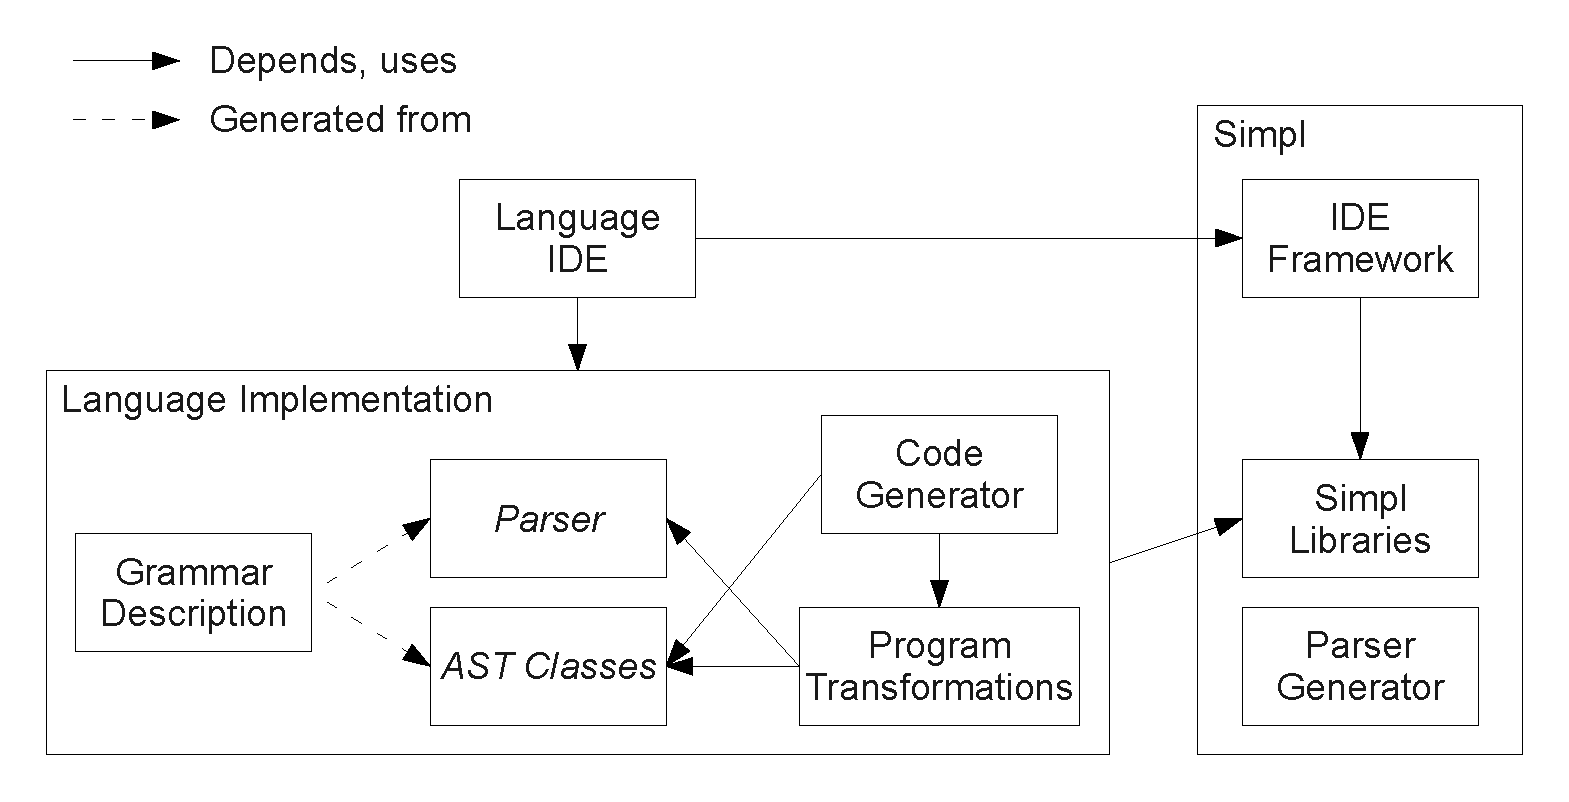
\includegraphics[width=0.7\columnwidth]{simpl/architecture}
\par\end{centering}

\caption{\label{fig:architecture}Architecture of a DSL implemented with Simpl.
Components with captions in italic are automatically generated.}

\end{figure}


Figure~\ref{fig:architecture} shows the main components of a DSL
implementation created with Simpl. The first part is the non-visual
language implementation that can be embedded into a bigger system.
Development of a new DSL starts with grammar description that specifies
both the context-free grammar of the DSL and the classes for representing
the abstract syntax tree (AST) of a DSL program. The Simpl parser
generator takes the grammar description as input and produces a parser
and the AST classes. The (optional) program transformation component
takes as input an AST and checks or transforms it. The code generator
converts the preprocessed AST to text. The second part of the DSL
implementation is the language IDE. It builds on Simpl IDE framework
and the non-visual part of the language implementation.


\subsection{Scanning and Parsing}

In Simpl, the grammar description is used to generate both the parser
and Scala case classes that are used to express the abstract syntax
tree (AST) of the DSL program. By default, the AST class and attribute
names are derived from rule names. The developer can add annotations
in the context-free grammar to modify the generated AST classes. As
an example, Figure \ref{fig:case-statement} shows set of rules for
parsing the Oberon0 \emph{CASE} statement. The identifiers before
the equals signs name the attributes in the case class that is used
for representing the AST. Figure \ref{fig:Automatically-generated-AST}
shows the Scala case classes that were generated from the example
rules. The attribute types are automatically derived from types of
called rules. If an attribute refers to rule(s) that can be called
multiple times, then the type of the attribute will be a list. For
example \emph{clauses} attribute in the \emph{CaseStatement} class
is typed as list because there can be more than one clause in one
case statement. Using the same attribute name several times in a rule
is allowed if the rule calls assigned to this attribute have compatible
type.

%
\begin{figure}[!h]
{\small }
\begin{lstlisting}[basicstyle={\footnotesize\ttfamily}]
CaseStatement:
    "CASE" expr=CompExpr "OF"
        clauses=CaseClause ("|" clauses=CaseClause)*
        ("ELSE" elseClause=StatementSequence)?
    "END";

CaseClause:
    items=CaseConstant ("," items=CaseConstant)* ":"
        stmt=StatementSequence;

CaseConstant: begin=SimpleExpr (".." end=SimpleExpr)?;
\end{lstlisting}
{\small \par}

\caption{\label{fig:case-statement}Grammar rules for parsing the Oberon0 \emph{CASE}
statement.}

\end{figure}


%
\begin{figure}[!h]
{\small }
\begin{lstlisting}[basicstyle={\footnotesize\ttfamily}]
case class CaseStatement(
    var expr: Expression, 
    var clauses: List[CaseClause], 
    var elseClause: StatementSequence) extends Statement

case class CaseClause(
    var items: List[CaseConstant],
    var stmt: StatementSequence)

case class CaseConstant(
    var begin: Expression, 
    var end: Expression)
\end{lstlisting}
{\small \par}

\caption{\label{fig:Automatically-generated-AST}AST classes for expressing
the Oberon0 \emph{CASE }statement.}

\end{figure}


Simpl allows modifying the generated AST classes using return expressions.
Return expressions can specify return type of a rule and/or a Scala
expression that is used to compute the actual AST node returned by
the rule. In the Oberon0 implementation, return expressions were used
to make the AST more regular and uniform. Figure \ref{fig:Using-return-expressions}
shows two examples. The first rule ensures that the use of parentheses
does not introduce additional wrapping of the AST nodes. The second
rule makes all the unary expressions use a common AST class \emph{Unary(operation,~expression)}
so that they can be uniformly treated in the processing code. 

%
\begin{figure}[!h]
{\small }
\begin{lstlisting}[basicstyle={\footnotesize\ttfamily}]
ParenExpr returns Expression {expr}: "(" expr=CompExpr ")";

NotExpr
    returns Expression {Unary(UnaryOp.Not, expr)}
    : "~" expr=Factor;
\end{lstlisting}
{\small \par}

\caption{\label{fig:Using-return-expressions}Example rules using return expressions.
Rule \emph{ParenExpr} does not wrap the inner AST node. Rule \emph{NotExpr}
returns manually created AST class.}

\end{figure}






In addition to return expressions, Simpl supports adding attributes
and methods to AST classes. For example, the code for parsing identifiers
is shown in Figure \ref{fig:Adding-properties}. This code modifies
the normally generated \emph{Id} class to add attributes for storing
references to definition of this identifier, pre-calculated constant
values if this identifier evaluates to constant expression, and information
whether the identifier is a by-ref procedure parameter. These attributes
are filled out and used during name, type checking and code generation.

%
\begin{figure}[!h]
{\small }
\begin{lstlisting}[basicstyle={\footnotesize\ttfamily}]
terminal Id {
    // What does this identifier point to?
    var ref: Id = null
    // If this is constant, then what is its value?
    var constVal: Option[Int] = None
    // Used for "VAR" parameters.
    var byRef: Boolean = false
    def isByRef = byRef || ((ref ne null) && (ref.byRef))
} : ('a'..'z'|'A'..'Z') ('a'..'z'|'A'..'Z'|'0'..'9')*;
\end{lstlisting}
{\small \par}

\caption{\label{fig:Adding-properties}Rule for parsing identifiers. The generated
class \emph{Id} is amended by adding properties and methods to it.}

\end{figure}



\subsection{Name Analysis}

Simpl has no direct support, therefore the name analysis for the Oberon0
language was written in Scala. The implementation is quite straightforward:
it walks through the AST and for each identifier fills out its \emph{ref}
attribute (points from identifier, such as variable reference, to
declaration of this identifier. See also Figure \ref{fig:Adding-properties}).
During the walk, we maintained an environment: a mapping from identifier
names to declarations.






\subsection{Type Checking}

Like name analysis, type checking was implemented in Scala. Since
name analysis was run before type checking, there was no need to use
environments (mappings from names to types). Instead, the type checker
first attached type information to all the declared identifiers (variables,
constants, procedure parameters). It then propagated the type information
to all expressions and procedure calls and checked the types of operation
arguments and procedure call parameters.  According to task definition,
checking for negative array sizes was also part of type checking,
therefore the type checker computed values of all constant expressions
and stored the values in the AST.




\subsection{Source-to-Source Transformation}

In order to simplify C code generation, the Simpl implementation transformed
Oberon0 programs to simplify Oberon0 language constructs that have
no direct equivalent in the C programming language. The first transformation
lifted nested procedures to top level. The second transformation replaced
\emph{CASE} statements with sequence of \emph{IF} statements.


\subsubsection{\label{sub:Procedure-Lifting}Procedure Lifting}

Procedure lifting used links created during the name analysis step
and performed in-place modifications of the AST. The task was accomplished
in three steps. First step consisted of scanning the AST and locating
all the nested procedures. Figure \ref{fig:Program-before-lifting}
shows an example Oberon0 program with the inner procedure highlighted.
In the second step, all the nested procedures were lifted to top level.
The new name was formed by concatenating names of outer and inner
procedures. If the concatenation did not produce unique name, a number
was added to the name. Figure \ref{fig:Program-during-lifting} shows
the results of this step with the lifted procedure highlighted. Finally,
the AST was scanned and all identifiers that referenced the lifted
procedures were renamed to reflect the new names. Figure \ref{fig:Program-after-lifting}
shows the end result with the renamed identifier highlighted.

%
\begin{figure}[!h]
\begin{tabular}{>{\centering}p{0.33\textwidth}>{\centering}p{0.33\textwidth}>{\centering}p{0.33\textwidth}}
{\scriptsize }
\begin{lstlisting}[basicstyle={\footnotesize\ttfamily},escapechar={\%},showlines=true]
PROGRAM Foo;
    PROCEDURE Bar;
        %\texttt{\textbf{PROCEDURE Baz;}}%
        %\texttt{\textbf{END Baz;}}%
    BEGIN
        Baz
    END Bar;
BEGIN
    Bar
END Foo.
 
\end{lstlisting}
{\scriptsize \par}

\subfloat[\label{fig:Program-before-lifting}]{} & {\scriptsize }
\begin{lstlisting}[basicstyle={\footnotesize\ttfamily},escapechar={\%}]
PROGRAM Foo;
    %\texttt{\textbf{PROCEDURE BarBaz;}}%
    %\texttt{\textbf{END BarBaz;}}%
 
    PROCEDURE Bar;
    BEGIN
        Baz
    END Bar;
BEGIN
    Bar
END Foo.
\end{lstlisting}
{\scriptsize \par}

\subfloat[\label{fig:Program-during-lifting}]{} & {\scriptsize }
\begin{lstlisting}[basicstyle={\footnotesize\ttfamily},escapechar={\%}]
PROGRAM Foo;
    PROCEDURE BarBaz;
    END BarBaz;
 
    PROCEDURE Bar;
    BEGIN
        %\texttt{\textbf{BarBaz}}%
    END Bar;
BEGIN
    Bar
END Foo.
\end{lstlisting}
{\scriptsize \par}

\subfloat[\label{fig:Program-after-lifting}]{}\tabularnewline
\end{tabular}

\caption{Three stages of procedure lifting: locating nested procedures (a),
lifting the procedures (b), and renaming the procedure references
(c).}

\end{figure}



\subsubsection{\label{sub:Simplifying-CASE-Statements}Simplifying \emph{CASE} Statements}

The Oberon0 \emph{CASE} statement is more powerful than \emph{switch}
statement in C programming language as it has support for ranges.
In order to simplify code generation, we transformed Oberon0 \emph{CASE}
statements to series of \emph{IF}-\emph{ELSE }statements (see Figure
\ref{fig:CASE-statement} for an example transformation). We generate
new variable for storing the \emph{CASE} condition. Because the results
of \emph{CASE} simplification will go straight to C code generation,
we can optimize by not making the generated identifier \emph{gen\_1}
a legal Oberon0 identifier. This way we do not have to ensure that
it does not clash with any identifiers in this scope.

%
\begin{figure}[!h]
\begin{tabular}{>{\centering}p{0.35\textwidth}>{\centering}p{0.55\textwidth}}
{\footnotesize }
\begin{lstlisting}[basicstyle={\footnotesize\ttfamily},showlines=true]
CASE foo + bar OF
      1 : Write(1)
    | 3..4 : Write(34)
ELSE
    Write(-1)
END;
 
 
  
 
\end{lstlisting}
{\footnotesize \par}

\subfloat[\label{fig:case-before}]{} & {\footnotesize }
\begin{lstlisting}[basicstyle={\footnotesize\ttfamily}]
VAR gen_1: INTEGER;
...
gen_1 := foo + bar;
IF gen_1 = 1 THEN
    Write(1)
ELSE IF gen_1 >= 3 AND gen_1 <= 4 THEN
    Write(34)
ELSE
    Write(-1)
END;
\end{lstlisting}
{\footnotesize \par}

\subfloat[\label{fig:case-after}]{}\tabularnewline
\end{tabular}

\caption{\emph{\label{fig:CASE-statement}Oberon0 CASE} statement before (a)
and after transformation (b).}

\end{figure}



\subsection{Code Generation}

When implementing C code generation, we decided to decouple translating
Oberon0 language constructs to C from outputting properly formatted
C code. This allowed us to concisely express the transformation between
Oberon0 AST to C AST without concerning the pretty-printing of C code.
First, we created Scala case classes for expressing abstract syntax
of the C language. Next, Oberon0 AST was transformed to C AST. Because
the more complicated Oberon0 constructs were previously simplified
(see the previous subsection), the translation was quite straightforward.
In the last step, the C AST was transformed to string using pretty-printing
library included in Simpl.

Figure \ref{fig:code-generation} illustrates the code generation
process with an example procedure for calculating factorial. Since
Oberon0 has no functions, the result is returned in a \emph{VAR} parameter.
Whereas AST of the Oberon0 \emph{FOR} statement (see Figure \ref{fig:code-generation}b)
corresponds to Oberon0 syntax, the translated \emph{for} statement
(see Figure \ref{fig:code-generation}c) corresponds to C syntax (initialization
and increment are statements, guard is an arbitrary expression). During
the translation, all the identifiers are prefixed with underscore
to prevent clashes with existing keywords.

%
\begin{figure}[!h]
\begin{tabular}{>{\raggedright}p{0.48\textwidth}>{\centering}p{0.48\textwidth}}

\begin{lstlisting}[basicstyle={\footnotesize\ttfamily},escapechar={\%}]
PROCEDURE Fact(
    n: INTEGER;
    VAR Res: INTEGER);
  VAR i: INTEGER;
BEGIN
  Res := 1;
  %\texttt{\textbf{FOR i := 1 TO n DO}}%
    %\texttt{\textbf{Res := Res * i;}}%
  %\texttt{\textbf{END}}%
END Fact;
\end{lstlisting}


(a) Oberon0 source before code generation. & 
\begin{lstlisting}[basicstyle={\footnotesize\ttfamily}]
ForStatement(
 Id(i),
 NumberLit(1),
 Id(n),
 null,
 StatementSequence(
  List(
   Assignment(
   Id(Res),
   Binary(*,Id(Res),Id(i))))))
\end{lstlisting}


(b) Oberon0 AST corrensponding to the highlighted \emph{FOR} statement.\tabularnewline

\begin{lstlisting}[basicstyle={\footnotesize\ttfamily}]
For(
 Assign(
  Id(_i,false),
  NumberLit(1)),
 Binary(
  <=,
  Id(_i,false),
  Id(_n,false)),
 Inc(_i,NumberLit(1)),
 Sequence(
  List(
   Assign(
    Id(_Res,true),
    Binary(
     *,
     Id(_Res,true),
     Id(_i,false))))))
\end{lstlisting}


(c) \emph{FOR} statement translated to AST representing a C program. & 
\begin{lstlisting}[basicstyle={\footnotesize\ttfamily},escapechar={\%},showlines=true]
void _Fact(int _n,int *_Res) {
  int _i;
  (*_Res) = 1;
  %\texttt{\textbf{for (\_i = 1; \_i <= \_n; \_i += 1) \{}}%
    %\texttt{\textbf{({*}\_Res) = ({*}\_Res) {*} \_i;}}%
  %\texttt{\textbf{\}}}%
}
 
 
 
 
 
 
 
 
 
 
\end{lstlisting}


(d) C source generated from the function in sub-figure (a). The highlighted
\emph{for} statement corresponds to AST from sub-figure (c).\tabularnewline
\end{tabular}

\caption{\label{fig:code-generation}Code generation example: translating the
procedure from Oberon0 to C.}

\end{figure}



\subsection{Artifacts}

The Oberon0 implementation is composed of five different artifacts
(A1, A2a, A2b, A3, A4). Each artifact either adds additional constructs
to the language or adds additional features, such as type checking,
procedure lifting or code generation. Table \ref{tab:loc-statistics}
shows code sizes for different artifacts and tasks. Code size is measured
in lines of code; empty lines and comments were not counted. For counting
lines of code, we used program \emph{cloc}%
\footnote{see \url{http://cloc.sourceforge.net/}%
} that was extended with support for Simpl grammar files. In the table,
each row represents size of a particular component:
\begin{itemize}
\item Parse -- Simpl grammar file and any additional Scala code (such as
custom classes for expressing binary operators and checks that numerical
constants fit into 32 bits);
\item Name -- code for name analysis;
\item Type -- code for type checking and and constant inlining%
\footnote{Constant inlining is used to check for negative array sizes.%
};
\item Lift -- code for lifting nested procedures to top level;
\item Gen -- code generator, including simplification of \emph{CASE} statements,
transforming Oberon0 AST to C AST, and pretty-printing C AST;
\item Pretty -- pretty-printing of Oberon0 code;
\item Other -- other supporting code, such as error handling, main functions,
etc.
\end{itemize}
%
\begin{table}[!h]
\caption{\label{tab:loc-statistics}Code sizes for different artifacts and
components. Sizes are expressed as non-blank, non-comment lines of
code.}


\noindent \centering{}\begin{tabular}{|c|r|r|r|r|r|r|r|r|}
\hline 
Artifact/Component & Parse & Name & Type & Lift & Gen & Pretty & Other & \textbf{Total}\tabularnewline
\hline
\hline 
A1 & 193 & 181 &  &  &  &  & 44 & \textbf{418}\tabularnewline
\hline 
A2a & 38 & 135 &  &  &  &  & 16 & \textbf{189}\tabularnewline
\hline 
A2b &  &  & 301 &  &  &  & 17 & \textbf{318}\tabularnewline
\hline 
A3 &  &  & 92 &  &  &  & 17 & \textbf{109}\tabularnewline
\hline 
A4 & 48 & 44 & 89 & 72 & 463 & 198 & 39 & \textbf{953}\tabularnewline
\hline 
\textbf{Total} & \textbf{279} & \textbf{360} & \textbf{482} & \textbf{72} & \textbf{463} & \textbf{198} & \textbf{133} & \textbf{1987}\tabularnewline
\hline
\end{tabular}
\end{table}


Except for A1, the artifacts are not self-contained in the terms of
code. The artifacts reuse grammar files and Scala code. Figure \ref{fig:artifact-dependencies}
shows the dependency graph between artifacts. The grammar files are
reused by using include directive. For example, L3 grammar includes
L2 grammar and overwrites production rules for declarations (by adding
procedure declaration) and statements (by adding procedure calls).
Services written in Scala, such as name analysis and type checking,
were extended using inheritance. In general, the extension consisted
in overriding \emph{processStatement}, \emph{processExpr} etc. methods
and adding new case clauses to process additional kinds of statements
or expressions.

%
\begin{figure}[!h]
\noindent \begin{centering}
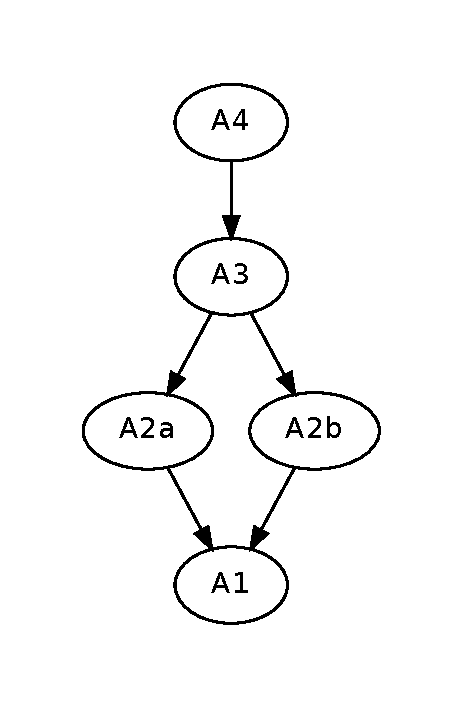
\includegraphics[scale=0.5]{simpl/artifacts}
\par\end{centering}

\caption{\label{fig:artifact-dependencies}Dependencies between artifacts in
the Oberon0 implementation.}

\end{figure}


In addition to artifacts mandated in the challenge, we used Simpl
to implement basic IDE for the Oberon0 language (see Figure \ref{fig:Screenshot-of-Oberon0}
for example screenshot). The IDE provided syntax highlighting, error
highlighting, outline view, hyperlinking, code folding, and occurrence
marking. The total code size for the IDE module was 106 lines, some
of which was filler. Most of the Oberon0-related functionality was
encapsulated in a 33-line class that contained IDE services. The IDE
code was based on the existing code checker (artifact A4) and did
not involve references to Eclipse APIs. 

%
\begin{figure}[!h]
TODO: screenshot.

\caption{\label{fig:Screenshot-of-Oberon0}Screenshot of Oberon0 IDE}

\end{figure}





\subsection{Observations}

First, it should be noted that Simpl is not directly targeted at creating
full-featured implementations of typical programming languages. Currently
the focus is on domain-specific languages and quite simple code generators.
Therefore, Simpl provided direct support for a subset of all the tasks
contained in this challenge. In particular, we used Simpl to create
a parser and class model for expressing AST of Oberon0 programs, and
for pretty-printing the AST. Although not included in challenge task,
we also used Simpl to create an IDE for the Oberon0 language.

Simpl currently uses ANTLR as a parser backend and therefore inherits
the use of \emph{LL(k)} parsing algorithm. The \emph{LL(k)} algorithm
has trouble expressing left-recursive grammar rules and thus parsing
left-associative operators. This limitation means that operator precedence
must be encoded in grammar rules%
\footnote{In this challenge the grammar was already specified in this form.%
} and it also results in cumbersome AST. The cumbersome AST can be
worked around by using return expressions that shape the AST nodes
returned by the grammar rules. In the future, we plan to use parser
backend that does not have this restriction.

Simpl grammar system is not specifically targeted at implementing
modular grammars. It only supports simple inclusion mechanism with
the ability to overwrite rules in the included grammars. In the challenge
exercise, this introduced minor code duplication. For example, in
order to introduce new kind of statement, one has to repeat the \emph{Statement}
rule with all the other preexisting statements. Overall, for the modularity
features were adequate for the current situation where there were
language levels with increasing complexity and each following level
added new constructs to the language. However, if the task were to
require highly modular grammars, then the current modularity features
likely would not have sufficed.


\subsection{Conclusions}

In general, implementing the challenge with Simpl was a straightforward
exercise. The grammar description was legible and the automatically
generated AST classes worked well with processing code written in
Scala. Simpl does not have support for implementing program checkers
and program tranformation, therefore these functions were written
in straight Scala. In addition to required tasks, we implemented an
IDE for Oberon0. The IDE was based on challenge code and required
minimal amount of effort to create.


% next line is used by my TeXShop environment; do not remove, Doaitse
% !TEX root = ../ldta_tool_challenge.tex
\newcommand{\doaitse}[1]{\marginpar{\textcolor{red}{\textbf{Doaitse:}#1}}}
\newcommand{\marcos}[1]{\marginpar{\textcolor{red}{\textbf{Marcos:}#1}}}

\newpage

\lstdefinelanguage{haskell}{
keywords={module, where, let, in, case, of, proc, rec, do, if, then, else, data, type, deriving},
sensitive=true
}
\newcommand{\haskellsize}{\fontsize{9pt}{9pt}}
\lstnewenvironment{haskell} 
{\lstset{language={haskell}}\haskellsize}{}
\lstset{
      basicstyle=\small\ttfamily,
      flexiblecolumns=false,
      tabsize=4,
      fontadjust= true,
      lineskip=0.7pt,
      aboveskip=\baselineskip,
      belowskip=\baselineskip,
      frame=tb,
      showspaces=false,
      showtabs=false,
      framerule=0.5pt,
      framexleftmargin=0.2cm,
      numbers=none,
      basewidth={0.5em,0.45em},
      literate={+}{{$+$}}1 {/}{{$/$}}1 {*}{{$*$}}1 {=}{{$=$}}1
               {>}{{$>$}}1 {<}{{$<$}}1  {\\}{{$\lambda$}}1
               {\\\\}{{\char`\\\char`\\}}1
               {->}{{$\rightarrow$}}2 {>=}{{$\geq$}}2 {<-}{{$\leftarrow$}}2
               {<=}{{$\leq$}}2 {=>}{{$\Rightarrow$}}2 
	       {<<<}{{$\lll$}}2 {>>>}{{$\ggg$}}2 {-<}{{$\prec{}$}}2
               {>>}{{>>}}2 {>>=}{{>>=}}2 {+>>}{{+>>}}2 {<|>}2
	       {|}{{$\mid$}}1 {iI}{{$\llfloor$}}1 {Ii}{{$\rrfloor$}}1
	       {undefined}{{$\perp$}}1 {\\\$}{{\$}}1 
       }
\newcommand\texthaskell[1]{{\lstinline[language={haskell}]{#1}}}
\newcommand\texthaskellF[1]{{\haskellsize\lstinline[language={haskell}]{#1}}}


\section{CoCoCo: Compositional Compiler Construction in Haskell}

\subsection{Introduction}

CoCoCo\footnote{Compositional Compiler Construction - \url{http://www.cs.uu.nl/wiki/bin/view/Center/CoCoCo}} is a set of libraries and tools in the form of a collection of embedded domain specific languages (EDSL) for constructing extensible compilers,
where compilers can be composed out of \emph{separately compiled}  
language-definition fragments. The Haskell type system  not only checks the expressions inside a component, but also the mutual consistency of a collection of components. Our approach builds on:
\begin{itemize}
%\item the introduction of typed abstract syntax \cite{BaSw02}
\item the possibility to represent mutually dependent 
recursive structures, such as context free grammars, and to inspect and manipulate such structures in a type-safe way \cite{BSV09}
\item the description of typed grammar fragments as first class Haskell values \cite{VSD12}
\item the definition of a typed Left-Corner Transform (LCT), which removes left-recursion from a grammar; this enables us
use top-down parsing techniques to build parsers out of grammar fragments \cite{BSV09b}
\item the possibility to construct a self-analysing, error correcting parser on the fly \cite{Swie2000,Swierstra08}
\item the possibility to deal with attribute grammars as first class  Haskell values, which can be transformed, composed and finally evaluated \cite{Viera:Attribute-Grammars,UU-CS-2011-028,VSM12}.
\end{itemize}

 

\subsection{Architecture}

The architecture of our implementation of Oberon0 is given in Figure~\ref{fig:modules};
boxes represent Haskell modules and arrows are \texthaskell{import} relations 
(e.g. the module \texthaskell{L4.SemT5} imports \texthaskell{L4.SemT3} and \texthaskell{L3.SemT5}).
Each module contains a collection of normal Haskell value definitions and can be compiled separately. 
The design is incremental:  rows corresponds to syntactic extensions (language levels) and
 columns corresponds to semantic extensions (tasks);
each artefact in the challenge corresponds to a dashed box containing the modules involved in that artefact.
\begin{figure}[th]
\begin{center}
	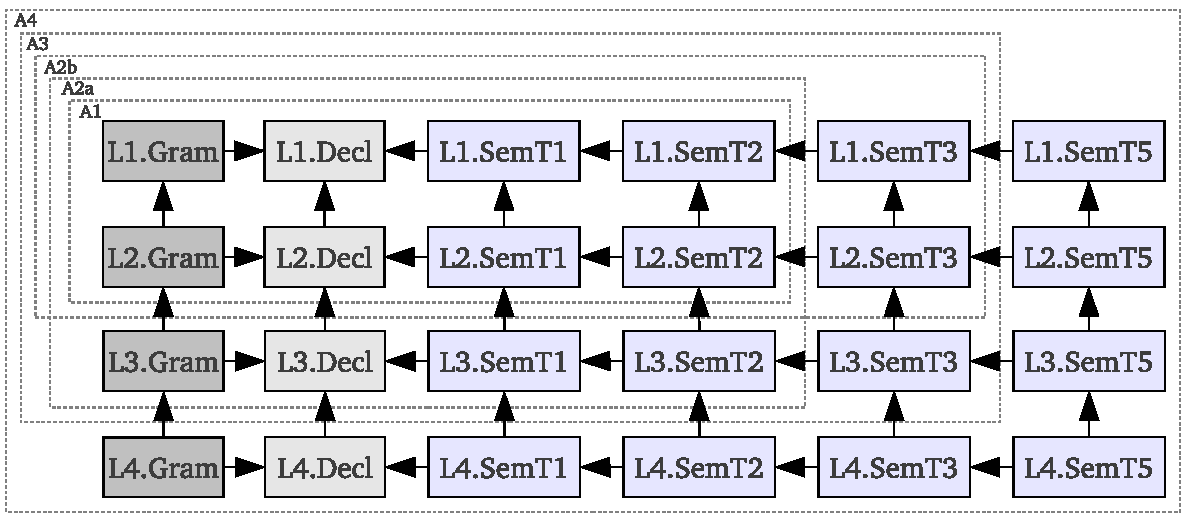
\includegraphics[scale=0.65]{cococo/modules.pdf}
\caption{Architecture of the Oberon0 Implementation}
\label{fig:modules}
\end{center}
\end{figure}
For each language level \texthaskell{L1} to \texthaskell{L4}: 
%
\begin{itemize}
	\item  \texthaskell{Gram} modules contain syntax definition in the form of first-class grammar fragments 
	%(i.e. \texthaskell{L1.Gram} contains \texthaskell{l1}, \texthaskell{L2.Gram} contains \texthaskell{l2}, etc.)
	\item \texthaskell{Decl} modules contain the definition of the type of the semantics' record, and thus the interface to the abstract syntax of the language at hand
	\item \texthaskell{Sem} modules implement the semantics of each task in the form of rules which together construct an attribute grammar
\end{itemize}
%
Notice that we do not include modules for Task 4. 
In Subsection~\ref{sec:agmacro} we  explain how we get this task done almost for free by using attribute grammar macros when defining \texthaskell{L2} .

To build a compiler, e.g. Artefact 4 (Figure~\ref{fig:A4}), we import the syntax fragments (\texthaskell{l1}, \texthaskell{l2}, 
\texthaskell{l3} and \texthaskell{l4} 
from \texthaskell{L4.Gram}) and their respective semantics (\texthaskell{l1t5}, 
\texthaskell{l2t5}, \texthaskell{l3t5} and \texthaskell{l4t5} from \texthaskell{L4.SemT5}), 
combine them and build the compiler in the form of a parser which calls semantic functions.
\begin{figure}[th]
\begin{minipage}[b]{0.5\linewidth}
\begin{center}
	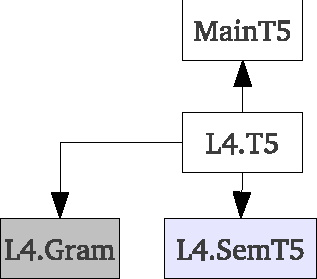
\includegraphics[scale=0.6]{cococo/main.pdf}
\caption{Architecture of Artefact 4}
\label{fig:A4}
\end{center}
\end{minipage}
\hspace{0.2cm}
\begin{minipage}[b]{0.5\linewidth}
\begin{haskell}
gl4t5 = closeGram \$ emptyGram +>> 
                    l1 l1t5   +>> 
                    l2 l2t5   +>> 
                    l3 l3t5   +>> 
                    l4 l4t5

pA4 = (parse . generate kws) gl4t5
\end{haskell}
\vspace{-15pt}
\caption{A Parser for Artefact 4}
\label{fig:pA4}
\end{minipage}
\hspace{0.5cm}
\end{figure}
In Figure~\ref{fig:pA4} we show how the parser of Artefact 4 is generated. 
The left-associative operator (\texthaskell{+>>}) takes as its left-hand side operand a grammar and as its right-hand side operand a  transformation to be applied.
We start with an empty grammar (\texthaskell{emptyGram}) and apply the different language extensions to it.
The function \texthaskell{closeGram} closes the constructed grammar and applies the \emph{left-corner transform} in order to remove potentially introduced left-recursion; 
as a consequence straightforward combinator-based top-down parsing techniques can be used in building the parser from the transformed grammar. 
Then \texthaskell{generate kws} generates a parser integrated with the semantics for the language starting from the first non-terminal,
where the list \texthaskell{kws} is a list of keywords extracted from the grammar description. 
This takes care of the problem that something which is an identifier in an earlier language may become keyword in an extended  language. 
The function \texthaskell{parse} finally  parses the input program and returns its semantics.
In the actual implementation of Oberon0 we construct scanner-less parsers using the uu-parsinglib\footnote{\url{http://hackage.haskell.org/package/uu-parsinglib}} parser combinator library;
%our library also provides  support for uulib\footnote{\url{http://hackage.haskell.org/package/uulib}} based parsers.

\subsection{Syntax}


Using our combinator library\footnote{MUtually Recursive Definitions Explicitly Represented - \url{http://hackage.haskell.org/package/murder}} \cite{VSD12} we represent  the concrete syntax of each language fragment as a Haskell value.
A fragment of the code that constructs the Context-Free Grammar (CFG) of the initial language L1 is given in Figure~\ref{fig:gram}, in which we recognise the underlying left-recursive context free grammar.
\begin{figure}[th]
\begin{center}
\begin{haskell}
l1 sf = proc _ -> do
   rec modul  <- addNT -< ...
       ...
       exp    <- addNT -< iI sexp   Ii <|> 
                          iI (pEExp     sf) exp  "=" sexp   Ii <|> ...
       sexp   <- addNT -< iI signed Ii <|> 
                          iI (pPlusExp  sf) sexp "+" signed Ii <|> ...
       signed <- addNT -< iI term   Ii <|> 
                          iI (pNegExp   sf) "-" term Ii <|> ... 
       term   <- addNT -< iI factor Ii <|> 
                          iI (pTimesExp sf) term "*" factor Ii <|> ...
       factor <- addNT -< iI (pIdExp    sf) ident Ii <|>  
                          iI (pIntExp   sf) int   Ii <|> ...
       ...
   exportNTs -< exportList modul \$ export cs_Expression exp ...
\end{haskell}
\vspace{-15pt}
\caption{Fragment of the concrete syntax specification of L1}
\label{fig:gram}
\end{center}
\end{figure}
Each grammar fragment consists of a sequence of grammar transformations expressed using Haskell's arrow syntax \cite{507664}, each of the form \texthaskell{output <- transformation -< input}. Each transformation is parameterised by \texthaskell{input} and updates the implicitly maintained grammar description binding additional results to \texthaskell{output}.
New non-terminals (syntactic category) of the CFG are introduced using  \texthaskell{addNT} transformations, which take as input an initial set of productions for that non-terminal and returns a value which may be used in other transformations to refer to this new non-terminal.  Each right hand side of a production (alternative) is expressed in so-called \emph{applicative style} \cite{McB07},
using idiomatic brackets\footnote{note that \texthaskell{iI} and \texthaskell{Ii} are plain Haskell values}  \texthaskell{iI} and \texthaskell{Ii} to delineate the list of components constituting an alternative. Note that the resulting  notation in Haskell closely resembles a similar description in a dedicated language.  The Haskell type of an element determines the role the element plays in the parsing process and the final semantics of the alternative: \texthaskell{String} values are e.g. interpreted as keywords to be recognised, and carry no semantic value of their own, functions do not require any parsing (i.e. correspond to the empty token sequence) but carry a value which is the function value itself (referring to the semantics associated to the abstract syntax nodes), 
and non-terminal references both have a parsing effect  and construct a semantic value.
Alternatives for the same non-terminal are combined with the \texthaskell{<|>} (choice) operator.

The semantics of an abstract syntax tree is represented by a Haskell function mapping inherited attributes to synthesised attributes; attribute grammar evaluation can be performed without explicit scheduling, since we implicitly make use of Haskell's lazy evaluation. In case attributes have a circular definition we take the least fixed-point semantics, which usually leads to an infinite structure. Fortunately this is no problem with Haskell as a host language.
The parameter \texthaskell{sf} in Figure~\ref{fig:gram}  contains the ``semantics of the language''; it is a record containing a semantic function for each productions, from which expressions like \texthaskell{pEExp sf} select the appropriate element. Such a semantic function computes the semantics of the recognised left hand side non-terminal of a production in terms of the semantics associated with the children of that production, which themselves are again functions mapping inherited to synthesised attributes.


Grammars defined in this way are \emph{extensible}, since further transformations may be applied to the grammar under construction, typically  in other modules.  
Each grammar exports (with \texthaskell{exportNTs}) its starting point (e.g. \texthaskell{modul}) and a table  of
\emph{exported non-terminals}, each consisting of a label (by convention of  the
form \texthaskell{cs_...}) and a reference to the current definition of that non-terminal in ht implicitly maintained record, again a plain Haskell value which can be used and modified in future extensions.

Figure~\ref{fig:gram2} contains a fragment of the definition of L2, 
which extends the L1 grammar with a \textoberon{CASE} statement.
\begin{figure}[th]
\begin{center}
\begin{haskell}
l2 sf = proc imported -> do
     let statement = getNT cs_Statement     imported 
     let exp       = getNT cs_Expression    imported 
     let mbelse    = getNT cs_MaybeElseStmt imported 
     ...
     rec addProds -< (statement,iI(pCaseStmt sf) "CASE" exp "OF" 
                                                 c cs mbelse "END"Ii)
     ...
     exportNTs -< imported
\end{haskell} 
\vspace{-15pt}
\caption{Fragment of the grammar extension L2}
\label{fig:gram2}
\end{center}
\end{figure}
We start by retrieving references to all non-terminals which are to be extended or used (using \texthaskell{getNT}) from the collection of\texthaskell{imported} non-terminals.
We add new productions to existing non-terminals with \texthaskell{addProds}; since this does not lead to references to new non-terminals the \texthaskell{output} part of the arrow construct is omitted.
New non-terminals can still be introduced as well using \texthaskell{addNT}.
The Haskell type-system ensures that 
the \texthaskell{imported} list indeed contains a table with entries \texthaskell{cs_Statement}, 
\texthaskell{cs_Expression} and \texthaskell{cs_MaybeElseStmt}, 
and that the types of these non-terminals coincide with their use in the semantic functions of
the extensions.

The definition in Figure~\ref{fig:gram2} may look a bit verbose, but this is caused by the interface having been made explicit. 
Using some Template Haskell this can  easily be overcome.


\subsection{Aspect Oriented Semantics}
The semantics of Oberon0 were implemented using the
AspectAG\footnote{\url{http://hackage.haskell.org/package/AspectAG}}
\cite{Viera:Attribute-Grammars} embedding of attribute grammars in Haskell.  
In order to be able to redefine attributes or to add new attributes later, 
it encodes the lists of inherited and synthesised attributes of a
non-terminal as an HList-encoded \cite{KLS04} value; each attribute is associated with a unique type which is used as an index in such a ``list''. The lookup process is performed by the Haskell class mechanism.  
In this way the \emph{closure test} of the attribute grammar
(each attribute has a single definition) is implicitly realised by the Haskell compiler when building the right instances of the classes.
Thus, attribute grammar fragments can be individually
type-checked, compiled, distributed and composed to construct a
compiler.  

\subsubsection{Pretty-Printing}

Pretty-printing is implemented by a synthesised attribute, 
called \texthaskell{spp}\footnote{By convention we use the prefix \texthaskell{i} and \texthaskell{s} for inherited and synthesised attributes, respectively.}, 
using the pretty-printing combinators provided by the uulib\footnote{\url{http://hackage.haskell.org/package/uulib}} package.

Attributes have to be defined for each production of the abstract syntax tree. 
For example, the following code defines the attribute \texthaskell{spp} for the production \texthaskell{CstDecl}, for declarations of constants.
%
\begin{haskell}
sppCstDecl = syn spp $ do 
               nm  <- at ch_id_CstDecl
               exp <- at ch_exp_CstDecl
               return $ value nm >#< "=" >#< exp # spp >|< ";"
\end{haskell}
%
The production has two children: \texthaskell{ch_id_CstDecl}, of type \texthaskell{(DTerm String)}\footnote{\texthaskell{DTerm a} is the type used by murder to represent \emph{attributed terminals} (i.e. identifiers, values); it encodes the value (\texthaskell{value}) and position in the source code (\texthaskell{pos}) of the terminal.},
and \texthaskell{ch_exp_CstDecl}, an expression node.
The besides combinator \texthaskell{(>#<)} is used to combine the string value of \texthaskell{ch_id_CstDecl}, the string \texthaskell{"="},
the pretty-printed value of the child \texthaskell{ch_exp_CstDecl} and the string \texthaskell{";"}.

We construct the semantic functions for the productions by applying the \texthaskell{knit} function to the
(composed) aspects of a given task. This function connects the local attribute flow of the production, as described by the composed aspects, with the flow from the inherited to the synthesised attributes of the children in order to construct the flow from the inherited attributes of the root node to its synthesised  attributes.
In the case of Task~1 the aspects of the production \texthaskell{CstDecl}  consist of the single attribute \texthaskell{spp}.
\begin{haskell}
aspCstDecl = sppCstDecl
\end{haskell}


\subsubsection{Name analysis}
Error messages produced by the name analysis are collected in 
a synthesised attribute called \texthaskell{serr}.
The default behaviour of this attribute for most  productions is to concatenate the errors produced by 
its children.
To capture this pattern we introduce a generic rule |serrRule| computing this attribute using the  function \texthaskell{use} from the AspectAG library, 
which takes as arguments the label of the attribute to be defined (\texthaskell{serr}), 
the Haskell list of non-terminals (labels) for which the attribute is to be defined (\texthaskell{serrNTs}), 
an operator telling how to  combine the attribute values (\texthaskell{++}), 
and a unit value to be used when none of the children has such an attribute (\texthaskell{[]::String}).
\begin{haskell}
serrRule = use serr serrNTs (++) ([] :: [String]) 
\end{haskell}
When a new name is defined we check for multiple declarations and at
name uses we check for incorrect uses or uses of undefined identifiers, producing error messages when appropriate.
The code below shows the definition of \texthaskell{serr} for the use of an identifier
represented by a production
\texthaskell{IdExp}, which has a child named \texthaskell{ch_id_IdExp} of type \texthaskell{(DTerm String)}.
\begin{haskell}
serrIdExp = syn serr \$ do 
    lhs <- at lhs
    nm  <- at ch_id_IdExp
    return \$ checkName nm (lhs # ienv) ["Var","Cst"] "an expression"
\end{haskell}
With the (plain Haskell) function \texthaskell{checkName} we lookup the name (\texthaskell{nm}) 
in the symbol table (inherited attribute \texthaskell{ienv} coming from the left-hand side)
and, if it is defined, we verify that the name represents either a variable (\texthaskell{"Var"}) 
or a constant (\texthaskell{"Cst"}) and generate  a proper error message if not.

The symbol table is implemented by the pair of attributes \texthaskell{senv} and \texthaskell{ienv}.
The synthesised attribute \texthaskell{senv} collects the information from the name declarations
and the inherited attribute \texthaskell{ienv} distributes this information through the tree.

In order to perform the name analysis, the type of the symbol table could have been 
\texthaskell{Map String NameDef}, which is a map from names to values of type \texthaskell{NameDef} 
representing information about the bound name. However, since we want to use the same symbol table
for future extensions, we keep the type ``non-closed'' by using a list-like structure:
\begin{haskell}
data SymbolInfo b a = SI b a
type NMap a = Map String (SymbolInfo NameDef a)
\end{haskell}
For the current  task the symbol table includes values of type \texthaskell{NMap a},
parametric in \texthaskell{a}, the ``the rest of the information we might want to store for this symbol''.
In the example below, for declarations of constants, the table consists of a map from the introduced name 
to a \texthaskell{SymbolInfo} which includes the information needed by the name analysis (constructed using \texthaskell{cstDef})
and some other (yet unknown) information, which is represented by the argument the rule receives:
\begin{haskell}
senvCstDecl r = syn senv \$ do  
                  nm <- at ch_id_CstDecl
                  return \$ Map.singleton (value nm) 
                                         (SI (cstDef \$ pos nm) r)
\end{haskell}
Similarly to how we used \texthaskell{use} for the default cases of synthesised attributes,
we can capture the behaviour of distributing an inherited attribute to the children of a production
with the function \texthaskell{copy} form the AspectAG library:
\begin{haskell}
ienvRule _ = copy ienv ienvNTs 
\end{haskell}

The various aspects introduced by the attributes are combined using the function \texthaskell{ext}:
\begin{haskell}
aspCstDecl r = senvCstDecl r `ext` ienvCstDecl r `ext` 
               serrCstDecl   `ext` T1.aspCstDecl
\end{haskell}
In this case, for the production \texthaskell{CstDecl}, we extend \texthaskell{T1.aspCstDecl}, 
which is imported from \texthaskell{L1.SemT1} and includes the pretty-printing attribute,
with the attributes implementing the name analysis task (\texthaskell{serr}, \texthaskell{ienv} and \texthaskell{senv}).

Once the attributes definitions are composed, the semantic functions for the productions may be computed using the function \texthaskell{knit}.
For example, the semantic function of the production \texthaskell{CstDecl} in the case of \texthaskell{L1.SemT2} 
is \texthaskell{knit (aspCstDecl ())}. The use of \texthaskell{()} (unit) here is just to ``close the symbol table'',
since the rest of the information is not needed by the rules of Task 2.

\subsubsection{Type checking}

Type error messages are collected in the synthesised attribute \texthaskell{sterr}.
For type checking we extend the symbol table with the type information (\texthaskell{TInfo}) of the declared names.
This is done by \emph{updating} the value of the attribute \texthaskell{senv} with the function \texthaskell{synupdM}, 
which is similar to \texthaskell{syn} but redefines it making use of its current definition. 
In the following example we update the symbol table information for the production \texthaskell{VarDecl},
where \texthaskell{sty} is an attribute defined for expressions and types, computing their type information:
\begin{haskell}
senvVarDecl' r = synupdM senv \$ do 
        typ <- at ch_typ_VarDecl
        return \$ Map.map (\ (SI nd _) -> (SI nd \$ SI (typ # sty) r))
\end{haskell}
The previous definition of the type information is just ignored and only used to indicate the type of the symbol table.
Thus, thanks to lazy evaluation, when extending the aspects of Task 2 we only need to pass  an undefined value of type \texthaskell{SymbolInfo TInfo a}, 
where \texthaskell{a} is the type of the new rest of the symbol table (for future extensions):
\begin{haskell}
undTInfo :: a -> SymbolInfo TInfo a
undTInfo = const undefined

aspVarDecl r = (senvVarDecl' r) `ext` sterrRule `ext` 
               (T2.aspVarDecl \$ undTInfo r)
\end{haskell}

To represent type information we have to deal again with the lack of open data types in Haskell,
since we want to keep some specific information for each of the types of the extensible type system we are implementing, and we have decided to resort to the use of Haskell's \texthaskell{Dynamic} type. 
A \texthaskell{TInfo}, with the information of a certain type, consists of:
the representation \texthaskell{trep} of the given type, encapsulated as a \texthaskell{Dynamic} value, 
a \texthaskell{String} with its pretty-printing (\texthaskell{tshow}), 
and a function \texthaskell{teq} that, given another type information indicates if the actual type is compatible
with the given one.
\begin{haskell}
data TInfo = TInfo { trep  :: Dynamic
                   , tshow :: String 
                   , teq   :: (TInfo -> Bool) } 
\end{haskell}
%\doaitse{we could make this a Maybe to represent unity?}
The main task we perform during type checking is to verify whether the 
actual type of an expression is compatible with the type expected by its context.
For example if the condition of an \textoberon{IF} statement has type \textoberon{BOOLEAN}.
\begin{haskell}
check pos expected got 
  = if (teq expected got) || (teq got unkTy) || (teq expected unkTy)
    then []
    else [show pos ++ ": Type error. Expected " ++ show expected ++
          ", but got " ++ show got]  
\end{haskell}
If either the expected or the obtained type is unknown (\texthaskell{unkTy}) 
we do not report a type error, because unknown types are generated by 
errors that have been already detected by the name analysis process.

A very simple case of type information is the elementary type \textoberon{BOOLEAN},
where we do not provide any extra information than the type itself.
Thus, the type representation is implemented with a singleton type \texthaskell{BoolType}.
\begin{haskell}
data BoolType = BoolType 

boolTy = let d   = toDyn BoolType
             bEq = (==) (dynTypeRep d) . dynTypeRep . trep . baseType   
         in  TInfo d "BOOLEAN" bEq	        
\end{haskell}
To construct the corresponding \texthaskell{TInfo} we convert a \texthaskell{BoolType} value 
into a \texthaskell{Dynamic} with the function \texthaskell{toDyn}.
A type is compatible with \textoberon{BOOLEAN} if its base type\footnote{In case of a user type, the type it denotes.}
is also \textoberon{BOOLEAN}, i.e. is compatible if both types are represented with \texthaskell{BoolType} values.
With the function \texthaskell{dynTypeRep} we extract a concrete representation of the type of the value inside a \texthaskell{Dynamic} 
that provides support for equality.

There exist some other cases were a more involved type representation is needed.
For example, in the case of \textoberon{ARRAY} we include the type information of its elements 
and the length of the array, if it can be statically computed.
\begin{haskell}
data ArrType = ArrType (Maybe Int) TInfo 
\end{haskell}
Then, by using the type-safe cast function \texthaskell{fromDynamic} we can get access to 
this information provided the dynamic typed value represents an array.
Thus, when trying to index a variable, we can for example check if the index is out of range;
in case the cast does not succeed we  indicate that the variable we are trying to access is not an array:
\begin{haskell}
checkSelArray pos ty ind
  = case (fromDynamic . trep . baseType) ty of
     Just (ArrType l _) -> checkIndex pos ind l
     _                  -> [show pos ++ 
                            ": Accessed variable is not an array"] 
\end{haskell}
We use the same technique to store information about the fields of a \textoberon{RECORD}
and the parameters of a \textoberon{PROCEDURE}.

\subsubsection{Source-to-source transformation}
\label{sec:agmacro}

In \cite{VS12} we extended AspectAG with an \texthaskell{agMacro} combinator that enables us
to define the attribute computations of a new production in terms of the attribute computations of existing productions.
We defined the semantics of the extensions of the language level L2 using this macro mechanism.
The \textoberon{FOR}-loop is implemented as a \textoberon{WHILE}-loop 
and the \textoberon{CASE} statement is defined in terms of an \textoberon{IF}-\textoberon{ELSIF}-\textoberon{ELSE} cascade.
In the cases were specialised behaviour is needed, like for example pretty-printing, it is still possible to redefine the attributes
involved on these aspects. As such, our mechanism is much more expressive than conventional macro mechanisms, which only perform a structure transformation. Using the library we get Task~4 almost for free.

Our approach is not very suitable for some other kind of source-to-source transformations like optimisations,
because we do not represent the AST with values (if we want to keep the AST extensible) and
we (still) do not have higher-order attributes.
Although a possible approach is to generate an AST of a fixed core language and perform 
the optimisations in this language.

\subsubsection{Code generation}

We generate the C abstract syntax representation provided by the package language-c\footnote{http://hackage.haskell.org/package/language-c}.
This package also includes a pretty-printing function for the abstract syntax.

Since ANSI C does not allow for nested functions  we have to lift  all the procedures, 
types and constants definitions to top-level when generating the C code required by the challenge (note that  the lifting as specified is trivial, 
since nested procedures in Oberon0 cannot refer to variables defined in the outer scope).%the exercise does not require bindings to be lifted properly).
In order to avoid name clashes with C keywords or due to the lifting process, we rename every identifier to make it unique.  
New names are composed by: a character \texthaskell{'_'} (assuring no clashes with C keywords),
the path (module and procedure names) to the scope were the name is defined and the actual name. 
Thus, if we have the following Oberon0 program:
\begin{oberon0}
MODULE A;
  VAR BC : INTEGER;
  PROCEDURE B;
    PROCEDURE C;
    END C
  END B
END A.
\end{oberon0}
The names are mapped: the variable name \texthaskell{BC} to \texthaskell{A_BC},
the procedure name \texthaskell{B} to \texthaskell{A_B} and
the procedure name \texthaskell{C} to \texthaskell{A_B_C}.
Since underscore is not allowed in Oberon0 identifiers, 
this renaming does not introduce new clashes, 
like the one we could have had with \texthaskell{C} if the variable 
\texthaskell{BC} was called \texthaskell{B_C}.


To implement the renaming we extend the symbol table with the name mapping.
Thus, for example, when defining the code generation attribute for the
production \texthaskell{IdExp} (use of identifiers) the new name is looked-up in the table.

\subsection{Artefacts}

In Table~\ref{table:locs} we show the complexity (in lines of code without comments) of our implementation of the compiler,
disaggregated into the different tasks and language levels.
The \emph{Common} column includes the \texthaskell{Gram} and \texthaskell{Decl} files,
while the \emph{Common} row includes some code used by the \texthaskell{Main} modules.
\begin{table}\centering
\begin{tabular}{ | c || c | c | c | c | c | c | }
  \hline                        
  \emph{Lang. / Task} & \emph{Common} & \emph{T1} & \emph{T2} & \emph{T3} & \emph{T5} & \emph{Total} \\
  \hline                        
  \hline                        
  \emph{Common} & - & 42 & 14 & - & 23 & 79  \\
  \hline                        
  \emph{L1} & 128 & 156 & 147 & 220 & 228 & 879  \\
  \hline  
  \emph{L2} & 187 & 98 & 69 & 65 & 56 & 475  \\
  \hline  
  \emph{L3} & 94 & 75 & 75 & 134 & 145 & 523  \\
  \hline 
  \emph{L4} & 48 & 67 & 56 & 197 & 95 & 463  \\
  \hline 
  \emph{Total} & 457 & 438 & 361 & 616 & 547 & 2419  \\
  \hline 
\end{tabular}
\caption{Code sizes (in lines of code) of the components of the compiler}
\label{table:locs}
\end{table}

The code includes 26 lines of Template Haskell, calling functions defined in the libraries to avoid some boilerplate.

We have implemented all the combinations from L1-T1 to L4-T5, including the artefacts proposed by the challenge.

%\subsection{Observations}


\subsection{Conclusions}

The most important aspect of our approach is the possibility to construct a compiler 
out of a collection of pre-compiled, statically type-checked, possibly mutually dependent
language-definition fragments written in Haskell, but with a DSL taste.

When looking at all the aspects we have covered, 
we can conclude that we managed to find solutions for all of them. 
This should not come as a surprise since we could always fall back to plain Haskell in those cases where 
our libraries were not providing a standard solution for the problem at hand. 
We have seen such solutions for dealing with flexible symbol tables, generating new identifiers and types.

We mention again that our implementation is somewhat verbose, since each module contains quite some code ``describing its interface'' in the collection of co-operating modules. 
This is the price we have to pay for getting the extreme degree of flexibility we are providing. 
By collapsing the modules the amount of linking information shrinks considerably.
We can reduce verbosity even further by using the conventional attribute grammar system \emph{uuagc} to generate AspectAG code \cite{VSM12}.

Another cause of the verbosity is that we have not used the system itself nor Template Haskell to capture common patterns. 
We have chosen to reveal the underlying mechanisms, the role of the type system, the full flexibility provided, 
and have left open the possibility for further extensions.

The lack of open data types in Haskell make it not entirely straightforward to implement AST transformations in extensible languages using our technique.
Semantic macros solve some of these problems. A possible approach is to use our technique to implement the front-end of a compiler,
translating to a core fixed language, and then use other more traditional approaches (like uuagc) to implement the back-end.



\section{Comparison of implementations}
\label{sec:comparison}
\begin{itemize}
\item Quantitative comparison (LoC)
\item Qualitative comparison
\end{itemize}

\section{Observations}
\label{sec:observations}

\section{Conclusions}
\label{sec:conclusions}



\appendix

\section{Oberon 0 code}
\label{sec:samples}
Appendix contains example of Oberon code with line numbers


%% The Appendices part is started with the command \appendix;
%% appendix sections are then done as normal sections
%% \appendix

%% \section{}
%% \label{}

%% References
%%
%% Following citation commands can be used in the body text:
%% Usage of \cite is as follows:
%%   \cite{key}          ==>>  [#]
%%   \cite[chap. 2]{key} ==>>  [#, chap. 2]
%%   \citet{key}         ==>>  Author [#]

%% References with bibTeX database:

%\bibliographystyle{model1-num-names}
\bibliographystyle{elsarticle-num}
\bibliography{main,silver/silver,jastadd/jastadd,ocaml/ocaml,kiama/kiama,simpl/simpl,cococo/cococo,rascal/rascal}

%% Authors are advised to submit their bibtex database files. They are
%% requested to list a bibtex style file in the manuscript if they do
%% not want to use model1-num-names.bst.

%% References without bibTeX database:

% \begin{thebibliography}{00}

%% \bibitem must have the following form:
%%   \bibitem{key}...
%%

% \bibitem{}

% \end{thebibliography}


\end{document}

%%
%% End of file `elsarticle-template-1-num.tex'.
